%\documentclass[11pt]{hepthesis}
\documentclass[hyperpdf,11pt]{hepthesis}
%\documentclass[hyperpdf,bindnopdf,11pt]{hepthesis}

\usepackage{mathpazo}
\usepackage{xspace}
\usepackage{siunitx}
\usepackage[utf8]{inputenc}

% Acronyms
\newcommand{\CMS}{CMS\xspace}
\newcommand{\ATLAS}{ATLAS\xspace}
\newcommand{\LHC}{LHC\xspace}
\newcommand{\CERN}{CERN\xspace}
\newcommand{\WLCG}{WLCG\xspace}
\newcommand{\ECAL}{ECAL\xspace}
\newcommand{\HCAL}{HCAL\xspace}
\newcommand{\LINACTWO}{LINAC2\xspace}
\newcommand{\PSBooster}{PS Booster\xspace}
\newcommand{\PS}{PS\xspace}
\newcommand{\SPS}{SPS\xspace}
\newcommand{\BSM}{BSM\xspace}

% Physics symbols
\newcommand{\lumi}{\ensuremath{\mathcal{L}}\xspace}
\newcommand{\mom}{\ensuremath{p}\xspace}
\newcommand{\pt}{\ensuremath{\mom_{\text{T}}}\xspace}
\newcommand{\dphi}{\ensuremath{\Delta\phi}\xspace}
\newcommand{\deta}{\ensuremath{\Delta\eta}\xspace}

% Math shorthand
\newcommand{\aeta}{\ensuremath{|\eta|}\xspace}


%% PDF metadata
\makeatletter
\@ifpackageloaded{hyperref}{%
    \hypersetup{%
        %hidelinks=true,
        pdftitle = {Precision measurement of the Z invisible width with the CMS experiment}
        pdfsubject = {Shane Davy Breeze's PhD thesis},
        pdfkeywords = {CMS, Electroweak physics, Z boson, Precision measurement, LHC},
        pdfauthor = {\textcopyright\ Shane Davy Breeze},
        %linkcolor=black,
        %colorlinks=false
    }
}{}
\makeatother

\renewcommand{\listfigurename}{List of figures}
\renewcommand{\listtablename}{List of tables}

\title{Precision measurement of the \PZ invisible width with the \CMS experiment}
\author{Shane Davy Breeze}

\begin{document}
    \titlepage[Imperial College London\\Department of Physics]{
        A thesis submitted to Imperial College London\\
        for the degree of Doctor of Philosophy
    }
    \clearpage
    \pagenumbering{gobble}
The copyright of this thesis rests with the author. Unless otherwise indicated, its contents are licensed under a Creative Commons Attribution-Non Commercial 4.0 International Licence (CC BY-NC). Under this licence, you may copy and redistribute the material in any medium or format. You may also create and distribute modified versions of the work. This is on the condition that: you credit the author and do not use it, or any derivative works, for a commercial purpose. When reusing or sharing this work, ensure you make the licence terms clear to others by naming the licence and linking to the licence text. Where a work has been adapted, you should indicate that the work has been changed and describe those changes. Please seek permission from the copyright holder for uses of this work that are not included in this licence or permitted under UK Copyright Law.


    \begin{frontmatter}
        \begin{abstract}%
%
A precision measurement of the partial width of the Z boson decay to an invisible final
state is reported. Events from proton-proton collisions provided by the Large
Hadron Collider at a centre-of-mass energy of $\SI{13}{TeV}$ are collected by
the Compact Muon Solenoid experiment with the invisibly decaying Z bosons inferred from
a hadronic recoil. The data collected corresponds to a total integrated luminosity of $\SI{35.9}{fb^{-1}}$. The invisible width is measured to be
$512\pm\SI{16}{MeV}$, consistent with the standard model. This is a competitive result to previous measurements performed at the Large Electron Positron experiment. The measurement is systematically dominated by uncertainties associated with the measurement of
the energy scale of the recoiling hadronic system.
%
\end{abstract}%
        \begin{declaration}%
%
I hereby declare that the work contained within this thesis is my own. It is
produced on top of the existing work and ideas of several individuals and the
Compact Muon Solenoid collaboration as a whole. The work performed by others
is reviewed by the author, as key aspects in the later stages, in chapters 1--4. Although author contributions have been made to the hardware
trigger, they have been omitted in this thesis. Chapter 5 details the event
selection and categorisation designed by the author, although inputs are based
on work performed by others. Chapter 6 consists of work performed by CMS
collaborators and theoreticians, apart from the subsections discussing the
\ptmiss trigger efficiency and the \ptmiss calibrations. All remaining
chapters details the work done solely by the author.

In addition to the work presented, the author made key contributions to the analysis known as the $\alpha_{\mathrm{T}}$ search \cite{Sirunyan:2018vjp}.

The analysis is currently in the internal CMS review process, with a plan to
publish this measurement. All results shown are presented as the work
performed by the author and do not represent approved results by the CMS
collaboration.

\mbox{}\hfill Shane Davy Breeze.
%
\end{declaration}%
        \begin{acknowledgements}

This thesis represents the accumulation of the work that I have done in the past four years. None of this would have been possible without the support, guidance and encouragement I have received from many people, before and during my PhD. To all of you, I am truly thankful.

Firstly, I would like to acknowledge the STFC for providing the funding to allow me to pursue my ambitions. This includes the two terrific years spent out at CERN. And to the Imperial HEP group for accepting me within their research group for, what I believe, is a successful PhD.

I would like to thank my supervisor, Sarah Malik, for her guidance throughout my PhD and, in particular, her patience and encouragement pushing me further. Although the outcome may differ from our original plan, I still believe it is an exceptional result that would not have been possible without you.

I would also like to thank the CMS collaborators and colleagues I have worked closely with throughout the past four years. Although this thesis does not include the work I performed on the hardware trigger or the $\alpha_{\mathrm{T}}$ analysis, I am still grateful to both the Calo layer 2 and $\alpha_{\mathrm{T}}$ groups. In particular, I would like to thank Alex Tapper for his support and guidance which resulted in my work being published early on during my PhD. I would also like to thank Rob Bainbridge for his continual support during the height of the $\alpha_{\mathrm{T}}$ analysis, and after. And to Nick Wardle, thank you for the countless discussions that has helped my understanding of statistics, as well as our more general discussions.

Thank you to all my friends, old and new, who I have relied heavily upon not only with my work, but in keeping me grounded and helping me through the stressful times. I could not wish for a better group of friends.

To my Mum, thank you for all the support and encouragement throughout my whole life. You have been inspirational and have always believed in me. And thank you to my whole family; my dad, step-dad and siblings, for your support and interest in my work.
    
\end{acknowledgements}
        %\begin{preface}
    Preface
\end{preface}

        \tableofcontents
\listoffigures
\listoftables
%\frontquote{}{}

    \end{frontmatter}

    \begin{mainmatter}
        \cleardoublepage
        \pagenumbering{arabic}
        \chapter{Introduction}
\label{chap:introduction}

\pagenumbering{arabic}
%\chapterquote{}{}

The classification and description of fundamental particles and their
interactions by the standard model (SM) of particle physics has been
successfully confirmed by countless experiments. However, it lacks a
candidate for dark matter \cite{Ade:2015xua,Corbelli:1999af}, a neutrino
oscillation mechanism \cite{Fukuda:1998ah,Ahmad:2002jz,Eguchi:2002dm}, or
incorporating the gravitational interaction. At the LHC, the SM gained further
success upon the discovery of the Higgs boson
\cite{Aad:1471031,Chatrchyan:1471016}. Although numerous direct searches for
beyond the SM (BSM) have been performed, no clear signal of BSM physics has
been observed. As these searches continue to probe the extremities of
distributions for BSM physics, an alternative direction proceeds through
precision measurements of the SM, as presented in this thesis.

The SM predicts that about $20\%$ \cite{PhysRevD.98.030001} of the time a \PZ
boson decays into a neutrino-antineutrino pair. This decay constitutes the \PZ
invisible width, a signal not discernible in collider-based experiments.
Instead, it is inferred from the missing momentum associated with the invisible decay of the \PZ as it recoils against a detectable system. A measurement of the \PZ invisible width is a key test of the SM and can be translated into constraints on the number of neutrino species coupling to the \PZ boson. Deviations from the SM expectation may point towards the existence of new particles beyond the SM which contribute to the \PZ invisible width. Therefore, a precise measurement of this quantity could reveal signs of new physics

The experiments at LEP measured the invisible width of the \PZ using two
methods. The direct method measures the rate of an energetic photon recoiling
against an invisible system attributed to the s-channel \PZ production and
subsequent invisible decay with an associated initial state radiated (ISR)
photon: $e^+e^-\ra \gamma Z \ra \gamma\nu\bar{\nu}$. The indirect method
measures the total \PZ width, by studying the lineshape of the \PZ boson from
$e^+e^-$ collisions with a centre of mass energy near the \PZ mass, and
subtracts the partial widths to all visible final state. This method provides
the most precise measurement, with a sensitivity to BSM particles. A summary
of the measurements performed by the LEP experiments L3
\cite{Acciarri:1998vf}, OPAL \cite{Akers:1994vh} and ALEPH
\cite{Buskulic:1993ke} for the direct method, a combination and the indirect
measurement is shown in Tab.~\ref{tab:lep-zinv-width}.

\begin{table}[htb]
    \centering
    \begin{tabular}{cc}
         \hline\hline
         Experiment & $\Gamma_{\mathrm{inv}}$ (MeV) \\
         \hline
         L3 & $498\pm 12\pm 12$ \\
         OPAL & $539\pm 26\pm 17$ \\
         ALEPH & $450\pm 34\pm 34$ \\
         LEP combined & $503\pm 16$ \\
         \hline
         LEP indirect & $499.0\pm 1.5$ \\
         \hline
    \end{tabular}
    \caption{
        Summary of the measurements of the $\Gamma_{\mathrm{inv}}$ from the LEP experiments for the direct measurements (with the statistical and systematic uncertainties), its combination, and the indirect measurement.
    }
    \label{tab:lep-zinv-width}
\end{table}

To date, there is no published measurements of the \PZ invisible width at a
hadron collider. However, a precise measurement at the LHC complements the LEP
measurements through an independent test of the SM at a different energy
scale, exposing contributions to the invisible width to TeV scale
contributions. These additional contributions may come from couplings of the
\PZ with dark matter particles, such as the lightest supersymmetric candidate,
or a mixing between the neutrino and sterile neutrino states
\cite{Carena:2003aj}, to which both the direct and indirect measurements are
sensitive. However, the direct measurement is also sensitive to
contributions to the invisible final state without coupling to the \PZ boson,
such as a heavier mediator coupling to neutrinos or other exotic invisible
particles, or a four fermion interaction vertex \cite{Carena:2003aj}.
Therefore, both measurements are valuable tests of the SM with the direct
measurement a candidate for the LHC to provide a complementary measurement.

The experiment and analysis presented by the author is a direct measurement of
the invisible width of the \PZ boson with the CMS detector using data from
proton-proton collisions at ${\sqrt{s}=\SI{13}{TeV}}$ in 2016, corresponding
to an integrated luminosity of $\SI{35.9}{fb^{-1}}$. The measurement targets
the invisible decay of the \PZ bosons recoiling against a hadronic system. The
rate of the invisible final state is compared to the reference signal of the
partial widths to leptons (both electrons and muons) $\Gamma(\PZ\ra\ell\ell)$, since these decays are
kinematically similar. The invisible width is then given by
%
\begin{equation}\label{eq:zinv}
    \Gamma(\IZinv) = \frac{\sigma(\IZj)\mathcal{B}(\IZinv)}{\sigma(\IZj)\mathcal{B}(\IZll)}\Gamma(\IZll)\ ,
\end{equation}
%
where $\sigma(\IZj)$ is the cross section for the \IZj process, modified by
either the invisible branching fraction $\mathcal{B}(\PZ\ra\mathrm{inv.})$ or
dilepton branching fraction $\mathcal{B}(\IZll)$.
        \chapter{The Standard Model of Particle Physics}
\label{chap:theory}

%\chapterquote{}{}

\section{Introduction}

The standard model (SM) of particle physics is a quantum field theory description of the fundamental particles of matter and their interactions. The SM has been widely successful in its predictions, falling short in providing a dark matter candidate, including the existence of neutrino oscillations and incorporating gravitational interactions, among other possible discrepancies.  Nevertheless, it is the current best minimal description unifying the electromagnetic, weak and strong forces. In the quantum field theory, the equations of motion are determined from the Lagrangian through the principle of least action. Gauge theories provided the mathematical basis to embed physical symmetries within the model.

The SM has had many distinguishing successes since its conception. One of the most notable is the prediction of the Higgs boson \cite{PhysRevLett.13.321,PhysRevLett.13.508,PhysRevLett.13.585} and its subsequent discovery by the ATLAS \cite{Aad:2012tfa} and CMS \cite{Chatrchyan:2012xdj} experiments. The Higgs field is crucial in providing a mechanism for the apparent masses of the weak bosons, quarks and charged leptons whilst maintaining a gauge invariant theory.

This chapter will include an overview of the properties of the SM with particular detail on the quantum electrodynamic, quantum chromodynamic and electroweak sectors, leading to a discussion of the spontaneous symmetry breaking in the SM, known as the Higgs mechanism. This is followed by a discussion of the Monte Carlo techniques used to simulate the SM.


\section{Elementary particles}

The set of fundamental particles and interaction mediators within the SM is shown in Fig.~\ref{fig:particle}. This includes the quarks --- fermion constituents of protons and neutrons --- with three generations of up and down-type quarks with a charge of $+2/3$ and $-1/3$ (in units of the elementary charge). A quark also takes one of three colour states, the strong force equivalent of the electric charge. Through these colour states the quarks interact with the gluon colour octet via the strong interaction. In addition, the lepton sector consists of charged fermions which, in addition to the quarks, interact through the photon field leading to the electromagnetic interaction. Furthermore, all fermions --- quarks, charged leptons and neutral leptons (neutrinos) --- interact via the weak force, mediated by the \PW and \PZ bosons. A set of antiparticles mirror all the fermions leading to 12 fermion fields and an equal number of anti-fermion fields, split into 6 quarks and 6 leptons.

\begin{figure}[htb]
    \centering
    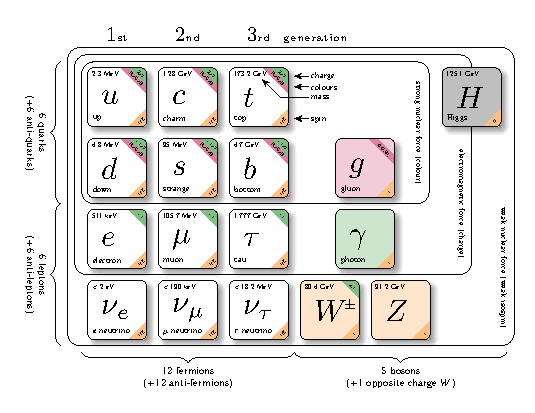
\includegraphics[width=0.8\textwidth]{diagrams/tikz/standard_model/standard_model.pdf}
    \caption[Summary of the standard model particles.]{
        Diagram of the particles within the SM including their quantum numbers such as charge, colour and spin, along with their measured masses. The left and right-handed chiral states are omitted and left for discussion in the main text.
    }
    \label{fig:particle}
\end{figure}


\section{Gauge theories}

In quantum field theory, the fundamental fields are unobservable. Instead, properties deriving from these fields, such as the cross section or rate of an interaction or decay, are measured. Many configurations of the underlying fields can give identical observable quantities. The transformation between these configurations is known as a gauge transformation and leaves the physical observables unchanged, hence these transformations are known as gauge invariant. Under Noether's theorem, a change in the field configuration which leaves the action, and hence the Lagrangian density, invariant is associated with conserved currents \cite{doi:10.1080/00411457108231446}.

\subsection{Quantum Electrodynamics}

Quantum electrondynamics (QED) is a gauge theory that sets out to describe the electron and the photon along with their interactions. The QED Lagrangian density consists of a Dirac field, the electron; a vector field, the photon, derived from Maxwell's equations; and an interaction term between the electron and photon fields:
%
\begin{equation}
    \mathcal{L}_{\mathrm{QED}} = \mathcal{L}_{\mathrm{Dirac}} + \mathcal{L}_{\mathrm{Maxwell}}\ + \mathcal{L}_{\mathrm{int}}\ .
\end{equation}

Maxwell's equations of electromagnetism are obtained from the Euler-Lagrange equations applied to the Lagrangian
%
\begin{equation}
    \mathcal{L}_{\mathrm{Maxwell}} = -\frac{1}{4}F^{\mu\nu}F_{\mu\nu}\ ,
\end{equation}
%
where $F^{\mu\nu}=\partial^{\mu}A^{\nu}-\partial^{\nu}A^{\mu}$ \cite{Peskin:1995ev} for the 4-potential $A^{\mu}$ with an electric scalar potential time-like and magnetic vector potential space-like components.

The Dirac Lagrangian describes the equations of motion, through application of the Euler-Lagrange equations \cite{Troutman1983}, of a spin-half fermion field $\psi$. This field is represented as a four-component spinor which may be interpreted as the spin-up and down of the left and right-handed helicity states \cite{Peskin:1995ev}. To form Lorentz invariant quantities, required in the Lagrangian, the adjoint field is defined as $\bar{\psi}=\psi^{\dagger}\gamma^0$ where $\psi^{\dagger}$ is the Hermitian conjugate of $\psi$ and $\gamma^0$ is the time-like component of the Dirac gamma matrices. These matrices obey the anticommutation relation $\{\gamma^{\mu},\gamma^{\nu}\} = 2g^{\mu\nu}$, where $g^{\mu\nu}$ is the Minkowski space metric, leading to the Lorentz invariant quantities such as $\bar{\psi}\psi$ and $\bar{\psi}\gamma^{\mu}\psi$ \cite{Peskin:1995ev}. These quantities form the basis of the Dirac Lagrangian of a free spin-half fermion:
%
\begin{equation}
    \mathcal{L}_{\mathrm{Dirac}} = i\bar{\psi}\gamma^{\mu}\partial_{\mu}\psi - m\bar{\psi}\psi\ ,
\end{equation}
%
where $i\partial_{\mu}$ is the position-space representation of the 4-momentum $p_\mu$, and $m$ is the mass of the particle \cite{1928RSPSA.117..610D}.  $U(1)$ group transformations of the field
%
\begin{equation}
    \psi \mapsto e^{i\alpha}\psi
\end{equation}
%
are not physical observables since they cancel in the magnitude of the matrix element used to determine the rate or cross section of a process. The Lagrangian is already invariant to such global transformations. However, local transformations where $\alpha\mapsto\alpha(x)$ introduces a term to the Dirac Lagrangian given by
%
\begin{equation}
    \mathcal{L}_{\mathrm{Dirac}} \mapsto \mathcal{L}_{\mathrm{Dirac}}  - \bar{\psi}\gamma^{\mu}(\partial_\mu\alpha(x))\psi\ ,
\end{equation}
%
To enforce gauge invariance, this additional term must be removed by introducing an additional field to the Dirac Lagrangian with a $U(1)$ transformation which opposes the additional term. Therefore, a $U(1)$ gauge invariant electron field must include an interaction with this new field, which is the photon field. This interaction term is realised through gauge invariance as
%
\begin{equation}
    \mathcal{L}_{\mathrm{int}} = -g\bar{\psi}\gamma^{\mu}\psi A_{\mu}\ ,
\end{equation}
%
where $A_\mu$ transforms into $A_\mu - (\partial_\mu\alpha(x))/g$ under a local phase transformation with a coupling constant $g$ between the electron and photon interaction. The interaction term is absorbed into the definition of a gauge covariant derivative $D_{\mu} \equiv \partial_\mu +igA_\mu$ to give the full QED Lagrangian as
%
\begin{equation}
    \mathcal{L}_{\mathrm{QED}} = i\bar{\psi}\gamma^{\mu}D_{\mu}\psi - m \bar{\psi}\psi - \frac{1}{4}F^{\mu\nu}F_{\mu\nu}\ .
\end{equation}
%
Additional Dirac terms, with associated photon interactions, are included for all spin-half charged fermions of the \SM.


\subsection{Quantum Chromodynamics}

The QED Lagrangian does not include self interaction terms with the photon field $A_\mu$. The extension to include interactions of the form $A^{\mu}A^\nu\partial_\mu A_\nu$ and $A^4$ introduces us to the theory of the strong force --- quantum chromodynamics (QCD). QCD sets out to explain the quarks, gluons and their interactions. The quark model explains the plethora of mesons and baryons as bound states of two and three quarks, respectively.  These quarks have fractional electric charges of $+2/3$ and $-1/3$ with six flavours. Furthermore, to explain the baryon spectrum with the Fermi exclusion principle, one of three colour states is assigned to quarks with equivalent anti-quark colour states \cite{Peskin:1995ev}. The minimal symmetry of which the quark colour states may be invariant to belongs to the $SU(3)$ group.  Including the Dirac Lagrangian for the quark states and enforcing gauge invariance requires countering field interaction terms, similar to the interaction between the electron and photon. An $SU(3)$ rotation is represented by eight $3\times 3$ matrices, hence eight counter terms with an independent field are required. These represent the eight gluon states $A_{\mu,a}$ with $a\in\{1,2,\ldots,8\}$. Therefore, the QCD Lagrangian is given by
%
\begin{equation}
    \mathcal{L}_{\mathrm{QCD}} = i\bar{\psi}_f\gamma^{\mu}D_\mu\psi_f - m_f\bar{\psi}_f\psi_f - \frac{1}{4}F^{\mu\nu}_a F_{\mu\nu,a}\ ,
\end{equation}
%
where $\psi_f$ is the quark spinor state with flavour $f$. The covariant derivative and field strength tensor are extended to gluon equivalents as
%
\begin{equation}
    D^{\mu} = \partial^\mu - i g_{s}A^\mu_a t_a
\end{equation}
%
and
%
\begin{equation}
    F^{\mu\nu}_a = \partial^\mu A^\nu_a - \partial^\nu A^\mu_a + g_{s} f_{abc}A^\mu_b A^\nu_c\ ,
\end{equation}
%
where $g_{s}$ is the quark-gluon coupling strength, $t_a$ are the generators of the $SU(3)$ group and $f_{abc}$ appears from the non-commutative property of the generators: $[t_a,t_b]=if_{abc}t_c$, leading to gluon self-interaction vertices \cite{Peskin:1995ev}.

As a result of the QCD interactions the strong coupling constant $g_s$ decreases with the energy scale leading to two notable effects. The first is weak strength of the strong force at high energies, allowing perturbative calculations. Whereas at low energies the increasing strength leads to the confinement of quarks and gluons, preventing the existence of isolated color charged particles in normal conditions. This property is important in high energy particle collisions where outgoing quarks and gluons form into showers of hadrons, detected as a cone of hadronic activity \cite{Peskin:1995ev}.


\subsection{Electroweak physics}\label{sec:ew-theory}

Another realised symmetry is the invariance between up and down-type quarks.  However, this symmetry is broken by the weak force where left and right-handed fermions are treated differently. Instead the left-handed up and down-type quarks are symmetric under the weak interaction, grouped into doublets with an $SU(2)$ symmetry, and similarly for right-handed antiparticles. However, right-handed fermions and left-handed antifermions do not interact with the weak force, and hence form a singlet with a $U(1)$ symmetry. Therefore, the electroweak interaction is symmetric under $SU(2)\times U(1)$ transformations.  The modified covariant derivative requires three generators of the $SU(2)$ group and a single generator of the $U(1)$ group:
%
\begin{equation}
    D_\mu = \partial_\mu + i\frac{g}{2}W_\mu^i\sigma^i + g' Y_W B_\mu\ ,
\end{equation}
%
where $i$ labels the generators of the $SU(2)$ group, $2\times 2$ Pauli matrices $\sigma^i$, with associated field $W_\mu^i$ and coupling $g$; and $Y_W$ is the generator of the $U(1)$ group with the field $B_\mu$ and coupling $g'$. The $W_\mu^i$ and $B_\mu$ fields represent the physical photon, $W^{\pm}$, $Z^{0}$ bosons through the combinations \cite{Peskin:1995ev}
%
\begin{align}
    W_\mu^\pm & = \frac{1}{\sqrt{2}}\left(W_\mu^1 \mp i W_\mu^2\right)\ ,\\\nonumber
    Z^0_\mu & = \frac{1}{\sqrt{g^2+g'^2}}\left(g'W_\mu^3 + gB_\mu\right)\quad\mathrm{and}\\\nonumber
    A_\mu & = \frac{1}{\sqrt{g^2+g'^2}}\left(g'W_\mu^3 - gB_\mu\right)\ .
\end{align}
%
However, introducing mass terms for the \PW and \PZ bosons breaks the gauge invariance of the Lagrangian. Similarly, the broken symmetry between left and right-handed particles leads to gauge invariance breaking terms: $\hat{\psi}_L\psi_R$ and $\hat{\psi}_R\psi_L$, preventing quark mass terms. Instead, a process known as spontaneous symmetry breaking gives rise to these mass terms whilst remaining as a gauge invariant theory.


\subsection{Spontaneous symmetry breaking}

The spontaneous symmetry breaking in the electroweak sector provides mass terms for the \PW and \PZ bosons through the Higgs mechanism \cite{PhysRevLett.13.321,PhysRevLett.13.508,PhysRevLett.13.585}. A Lorentz scalar, isospin-doublet field $\phi$ obeying the $U(1)$ gauge symmetry is introduced with a quartic potential
%
\begin{equation}
    \mathcal{L}_{\mathrm{Higgs}} = (D_\mu\phi)^*(D^\mu\phi) +\mu^2|\phi|^2 - \lambda|\phi|^4\ .
\end{equation}
%
The covariant derivates include the weak fields for a gauge invariant Lagrangian. However, the vacuum expectation value of the field $\phi$ is non-zero and given by
%
\begin{equation}
    \langle \phi \rangle = \frac{1}{\sqrt{2}}
    \begin{pmatrix}
        0 \\ v
    \end{pmatrix}
\end{equation}
%
with $v^2=\mu^2/2\lambda$. The $\phi$ field can be rewritten in terms of two fields, $h$ and $\chi$, with no vacuum expectation values:
%
\begin{equation}\label{eq:phi}
    \phi = \frac{1}{\sqrt{2}}(v + h)e^{i\chi/v}\ .
\end{equation}
%
The vacuum state is symmetric in a $U(1)$ transformation, allowing for any $\chi$ terms to be absorbed by a redefinition of the $U(1)$ gauge transformation. Expanding out the Lagrangian with this redefinition introduces $h$ as a real scalar field with mass terms for the $h$, \PW and \PZ bosons of $\sqrt{2}\mu$, $gv/2$, and $(v/2)\sqrt{g^2+g'^2}$ respectively. The photon does not acquire a mass term, as required for the SM.

Since the $\phi$ field is an $SU(2)$ doublet a gauge invariant coupling with the left-handed lepton doublet $E_L$ and the right-handed singlet $e_R$ is included in the Lagrangian as
%
\begin{equation}
    -\lambda_e (\bar{E}_L \phi) e_R + \mathrm{h.c.}\ ,
\end{equation}
%
where h.c. represents the Hermitian conjugate of the terms already present and $\lambda_e$ is a new dimensionless coupling constant \cite{Peskin:1995ev}.  Again, expanding out the Lagrangian with Eq.~\ref{eq:phi} leads to lepton mass terms with $m_e = \lambda_e v/\sqrt{2}$. Similarly, the equivalent $SU(2)$ invariant coupling for the left-handed quark doublet $Q_L$ and right-handed singlets $d_R$ and $u_R$ is included in the Lagrangian as
%
\begin{equation}
    -\lambda_d (\bar{Q}_L\phi) d_R - \lambda_u \epsilon^{ab}(\bar{Q}_L\phi_b^{\dagger})u_R + \mathrm{h.c.}\ ,
\end{equation}
%
where $\epsilon^{ab}$ is a two-dimensional Levi-Civita tensor \cite{Peskin:1995ev}.  In a similar manner to the lepton fields, the quarks fields acquire mass terms with $m_d = \lambda_d v/\sqrt{2}$ and $m_u = \lambda_u v/\sqrt{2}$. Additional generations of quarks introduce mixing terms between the various generations of up and down-type quarks through \PW boson interactions with couplings determined by the $3\times 3$ unitary Cabibbo-Kobayashi-Maskawa (CKM) mixing matrix \cite{PhysRevLett.10.531,Kobayashi:1973fv}.

Neutrinos do not have a right-handed chiral state and hence no couplings to the $\phi$ field can be included without breaking a gauge symmetry. Therefore, the neutrinos are massless in the SM. However, the neutrino flavours mixing has been measured experimentally and included ad hoc into the SM through the Pontcorvo-Maki-Nakagawa-Sakata matrix\cite{Pontecorvo:1957qd,Maki:1962mu}, analogous to the CKM matrix.

In addition to the mass terms introduced through spontaneous symmetry breaking, the $h$ field couples to the \PW and \PZ with a coupling proportional to the fourth-power of their mass, to fermions to the square of their mass, along with a trilinear and quartic self coupling.


\section{Event simulation and generation}
% https://arxiv.org/pdf/1101.2599.pdf

The complexity involved with modern particle accelerators, colliders and detectors require the use of simulated events to interpret the results and validate our understanding of the SM and beyond. To avoid needlessly generating all possible events from a collision, only the processes of interest are simulated through Monte Carlo integration of multidimensional integrals to determine differential cross sections, and hence the scattering probabilities. Additional Monte Carlo techniques allows the sampling of these distributions to generate events.

Event simulation is based on perturbation theory where higher order diagrams are neglected in calculations to avoid expensive computations. However, ignoring the entire perturbation series leads to infrared and ultraviolet divergences \cite{Ellis:1991qj}. These are avoided through renormalisation techniques and introducing the factorisation $\mu_F$ and renormalisation $\mu_R$ scales. Physical observables should not depend on these quantities, however, limitations in the calculations lead to some dependence.


\subsection{Hadron collider physics}\label{sec:hadron-collider-physics}

In a proton-proton collider, the hard interaction cross section between parton $a$ and parton $b$ in each proton is factorised into \cite{Ellis:1991qj}
%
\begin{equation}
    \sigma = \sum_{a,b} \int_0^1 dx_a dx_b \int f_a(x_a,\mu_F)f_b(x_b,\mu_F) d\hat{\sigma}_{ab\rightarrow n}(\mu_F,\mu_R)\ ,
\end{equation}
%
where $x_a$ is the proton momentum fraction associated to parton $a$ and $x_b$ for parton $b$ in the other proton. The $f(x,\mu)$ are the parton distribution function which describe the momentum fraction for a particular parton within a proton. The parton cross section $\hat{\sigma}_{ab\rightarrow n}$ denotes the interaction of partons $a$ and $b$ to form a specific $n$-particle final state. This is determined from a matrix element calculation integrated over the available phase space for the outgoing particles, averaged over initial spin and colour states and scaled by the parton flux. The number of Feynman diagrams used in the matrix element calculation is determined from the accuracy required. Leading order (LO) refers to the lowest power in the strong and electroweak coupling constants, which often refers to tree-level diagrams. Next-to-leading order (NLO) generators include the next lowest power, with the inclusion of higher-order virtual and real-emission corrections. Although the electroweak coupling constant is relatively small, virtual gauge boson loops result in logarithms \cite{Sudakov:1954sw} that scale with the ratio of the centre of mass energy to the weak scale ($\SI{100}{GeV}$), and hence become large corrections at a TeV colliders and beyond. The order to which these logarithms are calculated in the perturbation series proceeds from the leading logarithm (LL) to the next-to-leading logarithm (NLL), and so on.

The choice of $\mu_F$ and $\mu_R$ are typically set by the scale of the interaction, such as the mass of an s-channel resonance, or transverse momentum of the primary outgoing particle. The scale of the interaction may also have further meaning on the initial and final-state parton showers, where care is taken to avoid double-counting particles between the matrix element calculation and parton showering. The impact of the choice of scale is determined by varying both $\mu_F$ and $\mu_R$ up and down by a factor, both uncorrelated and fully correlated. This rescaling is provided as an alternative event weight to propagate as a systematic uncertainty.

The parton distribution functions are typically determined from a fit between data and theory predictions. The evolution of these functions from low momentum scale measurements to energy frontiers is given by the DGLAP equations \cite{Altarelli:1977zs,Dokshitzer:1977sg,Gribov:1972ri}. The uncertainties associated with these measurements are propagated through to the generated events.

The fixed order calculations discussed are not sufficient at encapsulating the full picture of the scattering process. Higher order effects are included through parton showering where the fragmentation of partons is simulated, down to the hadronization at $\SI{1}{GeV}$ scales. This hadronization process confines coloured particles into bound neutral final states, typically resulting in a shower of hadrons from each energetic parton. These clusters of hadrons are grouped into jets as a physical observable in-place of the parton. Multiple jet algorithms define the set of rules to group final state particles into jets. These typically involve a requirement on a distance parameter between a pair of particles as well as the momentum assigned to each particle. The goal is to cluster particles whilst remaining insensitive to non-perturbative effects associated with collinear splitting and soft emission \cite{Buckley:2011ms}. The most prominent algorithm used by the CMS experiment is known as the anti-$k_t$ algorithm \cite{Salam:2009jx}. This algorithm iterates over all final state particles, applying a condition on the distance parameter
%
\begin{equation}
    d_{ij} = \min\left(p_{ti}^{-2},p_{tj}^{-2}\right)\frac{\Delta R_{ij}^2}{R^2}\ .
\end{equation}
%
where $p_{ti}$ and $p_{tj}$ are the transverse momentum of particles $i$ and $j$, $\Delta R_{ij}^2$ is the distance between particles $i$ and $j$ in the rapidity-azimuthal plane and $R$ is a chosen scale for the jets, typically set to $0.4$. Particles are combined into a jet if they satisfy this condition.


\section{Summary}

The SM is a gauge theory of the fundamental particles and their interactions, unifying the electromagnetic, weak and strong forces into a single consistent theory. The matter particles consist of the coloured spin-half quarks and leptons. Through the spontaneous symmetry breaking of the electroweak sector, the quarks and charged leptons, along with the \PW and \PZ bosons, acquire a mass with the introduction of a scalar field, the Higgs field.

Simulation and generation of events within the SM framework, and possible extensions, involve Monte Carlo integration and sampling technique to solve multidimensional integrals. The cross section of a proton-proton collision is factorised into the constituent parton interaction which requires the parton distribution functions and depends on the factorisation and renormalisation scales. After the matrix element calculation is performed, all final state partons undergo a showering procedure and hadronisation to form a jet of particles. These jets are clustered with the anti-$k_t$ algorithm.

        \chapter{The \LHC and \CMS detector} \label{chap:detector}

%\chapterquote{}{}

%------------------------------------------------------------------------------%
\section{Introduction}

% TODO: Careful of overlap with introduction chapter
The \LHC was built with the design goal of leading the energy frontier of high
energy physics. This led to the successful discovery of the Higgs bosons by
the \ATLAS \cite{Aad:1471031} and \CMS \cite{Chatrchyan:1471016} experiments.
Moreover, \BSM searches with these experiments continue to push stringent
limits on the possible parameter-space of theorised new physics scenarios.
Such discoveries and searches are only possible by the hugely complex
detectors and the \LHC accelerator complex, built and maintained by thousands
of Engineers and Physicists.

%------------------------------------------------------------------------------%
\section{The \LHC}

\subsection{Accelerator Complex}

Proton collisions at the \LHC start from the ionisation of hydrogen gas to
liberate the proton nuclei from their bound atomic states. Subsequently, the
protons are accelerated by the radio-frequency (RF) cavity based accelerator
\LINACTWO and injected into the \PSBooster\ --- four superimposed synchrotron
rings accelerating protons from ${\SI{50}{MeV}}$ to ${\SI{1.4}{GeV}}$ --- to
enhance the intensity of the proton injected into the \PS. The \PS is a
synchrotron with a radius of ${\SI{72}{m}}$ bending the proton beam into a
ring with energies up to ${\SI{25}{GeV}}$ before being injected into the \SPS.
Prior to this injection the proton beam is bunched into discrete packets of
protons about ${\SI{4}{ns}}$ long with an equal spacing of ${\SI{25}{ns}}$
required by the \LHC for a bunch crossing rate of ${\SI{40}{MHz}}$. The \SPS
is another synchrotron with a larger radius of ${\SI{6.9}{km}}$ to accommodate
the acceleration of protons up to ${\SI{450}{GeV}}$ for the extraction by the
\LHC. The whole accelerator complex, shown in Fig.~\ref{fig:LHC-Complex},
allows the \LHC to accelerate protons bunches up to energies of
${\SI{6.5}{TeV}}$ with a bunch crossing period of ${\SI{25}{ns}}$ and
luminosities of the order of ${\SI{e34}{cm^{-2}s^{-1}}}$ \cite{Bruning:782076}.

\begin{figure}[!htbp]
    \centering
    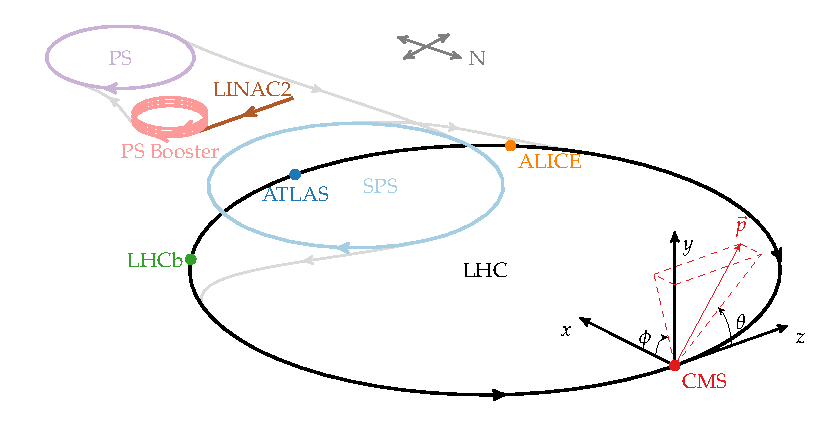
\includegraphics{diagrams/tikz/lhc_complex/lhc_complex.pdf}
    \caption{
        An isometric schematic view of the \LHC complex chain delivering
        proton-proton collisions at the four main detectors: \LHCb, \ATLAS,
        \ALICE and \CMS. The coordinate system used by the \CMS detector is
        shown in both cartesian and polar coordinates. The pseudorapidity
        $\eta$, defined as $-\ln(\tan(\theta/2))$, typically replaces the
        $\theta$ angle because of its convenient properties under Lorentz
        transformations. This diagram is not to scale and the relative
        positions of the rings are guides to the physical positions.
    }
    \label{fig:LHC-Complex}
\end{figure}


\subsection{\LHC Main Ring}

The main physics goals of the \LHC project was the discovery of the Higgs
boson, to observed new physics and rare \SM processes. The expected rate of a
particular process with a cross section $\xs$ at a integrated beam luminosity
$L$ is
%
\begin{equation}
    \mathcal{N} = L \xs \ .
\end{equation}
%
The event rate at the \LHC is directly controlled by the luminosity. For a
Gaussian distributed beam, the luminosity can be given in terms of beam
parameters as:
%
\begin{equation}
    \label{eq:beam-lumi}
    L = \frac{N_b^2 n_b\frev\relgamma}{4\pi\emitt\bstar} F\ ,
\end{equation}
%
where $N_b$ is the number of particles per bunch, $n_b$ is the number of
bunches per beam, \frev is the revolution frequency, \relgamma is the
relativistic gamma factor, \emitt is the normalised transverse beam emittance,
\bstar is the beta function at the collision point (related to the transverse
size of the beam) and $F$ is the geometric luminosity reduction factor due to
the crossing angle of each beam at the crossing point.

At the \LHC, the luminosity is maximised by tuning all parameters in
Eq.~\eqref{eq:beam-lumi}. This necessitated the use of proton beams
circulating in separate vacuum chambers and merging at insertion points to the
detectors. The beams nominally circulate in 2808 bunches with a spacing of
${\SI{25}{ns}}$ inside twin bore superconducting magnets --- two sets of coils
and beam channels within the same structure and cryostat --- achieving a peak
dipole field of ${\SI{8.33}{T}}$ to bend the beam. RF cavities apply the
potential gradient to accelerate the protons from ${\SI{450}{GeV}}$ to
${\SI{6.5}{TeV}}$. Quadrupole magnets focus the beam to suppress dispersion to
maintain the beam luminosity. Additional quadrupoles focus the beam as they
enter the collision sections and defocus as they exit  \cite{Bruning:782076}.


\section{Compact Muon Solenoid (\CMS) Experiment}

The conditions provided by the \LHC during 2016 data taking resulted in an
average number of collisions per bunch crossing of approximately 25, leading
to 1000 charged particles every ${\SI{25}{ns}}$ bunch crossing. The \CMS
detector \cite{Bayatian:922757} was designed to account for particle
multiplicities of this order by focusing on high-granularity subdetectors with
good time resolutions. This required a large number of detector channels and
millions of synchronised detector electronics, all with a high radiation
tolerance.

In addition to the conditions provided by the \LHC, the \CMS detector's design
was driven by four main physics requirements to achieve a broad range of
precision measurements and new physics searches, namely: searching for the
Higgs Boson, supersymmetric particles, new massive vector bosons, extra
dimensions; precision studies of the \SM; and heavy-ion physics. The physics
requirements are summarised as follows:

\begin{enumerate}
    \item \textbf{Muon identification:} ability to clearly identify muons up to
    $\aeta=2.4$ and dimuon mass resolutions of about $1\%$ for transverse
    momenta of \SI{100}{GeV}, with an unambiguous charge up momenta of
    \SI{1}{TeV}.
    \item \textbf{Charged particle reconstruction:} good momentum and
    reconstruction efficiency, particularly for the inner tracker, allowing
    for the identification of secondary vertices for the triggering and
    offline tagging $\tau$'s and $b$-jets. This requires a tracker component
    with a few cm of the interaction point.
    \item \textbf{Electromagnetic energy resolution:} measure the diphoton and
    dielectron mass with a resolution of $1\%$ for transverse momenta of
    \SI{100}{GeV} up to $\aeta=2.4$. In addition, efficiently reject backgrounds
    from \Ppizero decays into two photons and maintain prompt lepton isolation
    at high luminosities.
    \item \textbf{Transverse missing momentum and dijet mass resolution:} near
    complete reconstruction of the proton interaction to measure the
    transverse missing momentum. This requires a hermetic detector with hadron
    calorimeters extending up to $\aeta=5.0$ and fine component segmentation
    in the $\eta$-$\phi$ plane of less than $0.1\times 0.1$.
\end{enumerate}

The full design of the \CMS detector is shown in Fig.~\ref{fig:cms-full} which
achieves the requirements outlined above. The main distinguishing feature of
the \CMS detector is a ${\SI{3.8}{T}}$ superconducting solenoid magnet
enclosing the tracking and calorimetry subdetectors with and iron return yoke
to maintain a ${\SI{2}{T}}$ field outside the solenoid for the muon
subdetectors. All subdetectors are segmented into various regions in $\eta$
known as the barrel (covering the central $\eta$ range) and endcap (covering
up to $\aeta=3.0$, with a slight overlap with the barrel). The hadronic
calorimeter has an additional segment in the forward region, (covering
$3<\aeta<5$) as required for the missing momentum reconstruction. Further
subdetector dependent segmentation is done within the barrel, endcap and
forward regions; discussed in further detail in the following subsections.
This gives the \CMS detector a total length of ${\SI{21.6}{m}}$ and a diameter
of ${\SI{14.6}{m}}$ and weighing ${\SI{12500}{tons}}$.

\begin{figure}[htbp]
    \centering
    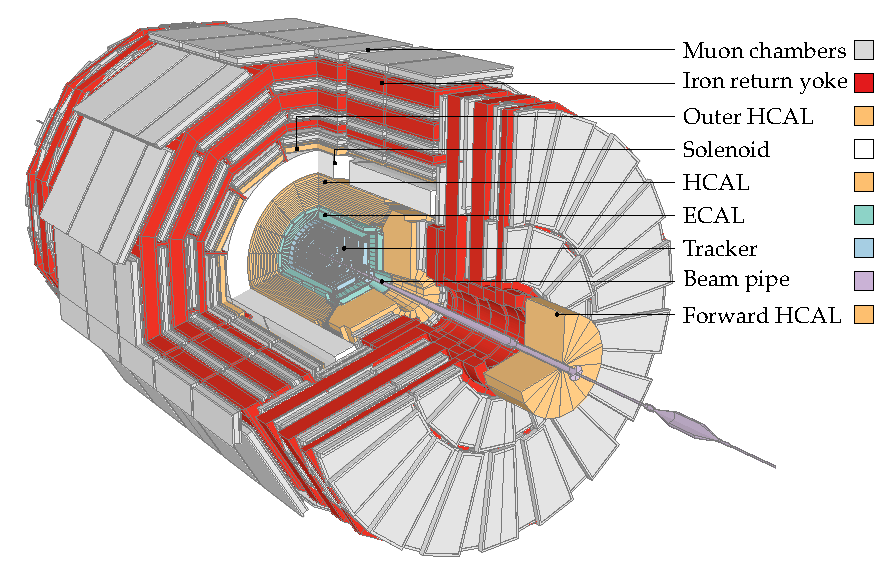
\includegraphics[]{diagrams/tikz/cms/annotated/cms_full.pdf}
    \caption{
        A schematic view of the \CMS detector and subdetectors with a section
        removed to view the internal components. Acronyms are explained in the
        text. The diagram was produced using the tools outlined in
        \cite{Sakuma:2013jqa}.
    }
    \label{fig:cms-full}
\end{figure}

\subsection{Silicon Tracker}

The inner most subdetector, the silicon tracker, measures the position of
charged particles from ionisation deposits (known as hits) across a
silicon-based reverse-biased p-n junction. A collection of hits is used to
reconstruct the curved trajectory, with a radius of curvature $r$, of the
particle with a charge $q$ within the magnetic field $B$ to determine the
momentum of the particle transverse to the field, \pt, given by:
%
\begin{equation}
    \pt = rqB\ .
\end{equation}
%
A collection of tracks may intersect at a common point leading to the
reconstruction of the primary interaction, pileup and secondary vertices.
These vertices are typically a few centimetres apart, therefore, the tracker
components are placed as near as ${\SI{4.4}{cm}}$ to the beam pipe.  The
silicon tracker, shown in Fig.~\ref{fig:cms-tracker}, consists of two main
components: pixels and strips. The pixels measure 3-dimensional positional
coordinates of hits for environments of high particle flux (up to 10 million
particles per second) near the beam. Pixel modules are aranged into three
layers placed in the barrel region (BPIX) at radii of ${\SI{4.4}{cm}}$,
${\SI{7.3}{cm}}$ and ${\SI{10.2}{cm}}$ with a length of ${\SI{53}{cm}}$,
centred on the z-axis. The pixel modules are staggered in the $\phi$-direction
to achieve an overlapping configuration. Two additional pixels layers are
placed in the both endcap regions (FPIX) with a turbine-like geometry with the
blades rotated by ${\SI{20}{\degree}}$ for overlapping blades. The overlap of
pixel modules ensures the charged particle passes through at least one module
in each layer. If two modules are hit the charge sharing between these modules
provides additional positional information on the hit leading to improved
position resolutions.

\begin{figure}[htbp]
    \centering
    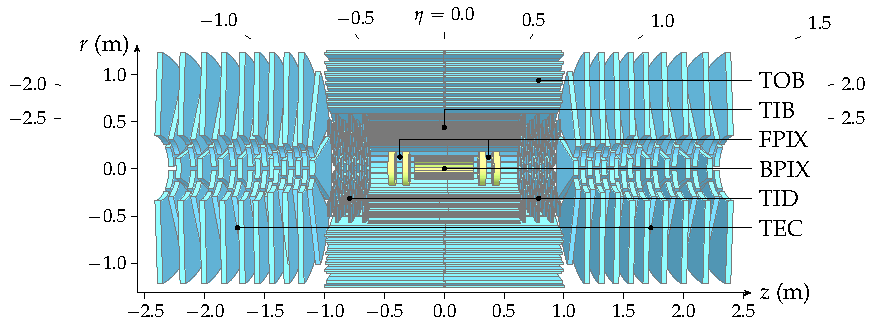
\includegraphics[]{diagrams/tikz/cms/annotated/cms_tracker.pdf}
    \caption{
        A cross-sectional view, in the $y$-$z$ plane, of the silicon tracker.
        The full tracker is shown in the upper part of the figure with a
        zoomed inset of the inner tracker in the central section and a further
        zoomed inset of the pixel tracker in the lowest part. The acronyms
        labelling various sub-components are defined in the text. The diagram
        was produced using the tools outlined in \cite{Sakuma:2013jqa}.
    }
    \label{fig:cms-tracker}
\end{figure}

Silicon strips are used further away from the beam pipe as the particle flux
reduces. Strips provide an accurate 2-dimensional position for hits, hence
layers are typically oriented in a stereo-configuration\footnote{A
stereo-configuration has layers rotated at an angle with respect to each other
to form a crosshatch pattern.} for the full 3-dimensional position. The
silicon strips are separated into an inner and outer component. The inner
component is further split by the barrel and endcap regions. The tracker inner
barrel (TIB) component consists of four layers positioned at a radius of
$20$--${\SI{55}{cm}}$ and covering ${|z|<\SI{65}{cm}}$ with cell sizes of
${\SI{10}{cm}\times\SI{80}{\micro m}}$. The first two layers use the
stereo-configuration with an angle of ${\SI{100}{mrad}}$. The tracker outer
barrel (TOB) component has six layers extending the coverage to
${|z|<\SI{110}{cm}}$ and ${\SI{55}{cm}<r<\SI{130}{cm}}$. Again the first two 
layers are place in a stereo-configuration with an angle of
${\SI{100}{mrad}}$. The inner endcap (TID) component provides coverage for the
gap between the TIB and TOB with three small disks oriented perpendicular to
the $z$-axis to avoid excessive shallow track crossing angles. The first two
disks have a stereo-configuration. The tracker outer endcap (TEC) consists of
nine disks extending into ${\SI{120}{cm}<|z|<\SI{280}{cm}}$ with
stereo-configuration for the first two  and the fifth disks
\cite{Borrello:687861}. The entirety of the silicon detector consists of 66
million pixels and 9.6 million silicon strips with near hermetic coverage up
to $\aeta=2.4$.

To process the data from the pixels and strips an on-detector chip processes
and buffers the analogue signal while waiting on a decision to accept or
reject the data (detailed in Sec.~\ref{sec:hardware-trigger}). Upon an accept
signal being received the data is transmitted over optical links to
off-detector chips for further processing, such as digitisation and data
formatting.


\subsection{\ECAL}

The \ECAL is a homogeneous calorimeter made of lead tungstate (\pbwo) crystals
designed to measure electromagnetic deposits (typically electrons and photons)
up to ${\aeta=3.0}$. The choice of lead tungstate scintillating crystals was
driven by their short radiation lengths, $X_0$ (${\SI{0.89}{cm}}$), and
Moliere radius \footnote{A radiation length is the distance travelled by a
particle through a material where, on average, the particle has lost $63.2\%$
of it's original energy. Similarly, the Moliere radius is the radius of a
cylinder which captures, on average, $90\%$ of the particle's shower,
transverse to the initial direction of travel.} (${\SI{2.2}{cm}}$) with fast
responses ($80\%$ of the light emitted is within ${\SI{25}{ns}}$) and have a
satisfactory level of radiation resistance. These properties allows a compact
design fully enclosed within the solenoid with sufficient containment of
electron and photon showers both laterally and along the length of the
crystals. The drawbacks of the crystal include low light yield
(${\SI{30}{photon/MeV}}$) requiring a coupling to photodetectors with
intrinsic gains operable in the magnetic field, and deterioration from
continuous irradiation monitored throughout.

The \ECAL is divided into the barrel section (EB) and the two endcap sections
enclosing the forward regions consisting of the endcap crystals (EE) and the
preshower (ES), diagrammatically shown in Fig.~\ref{fig:cms-ecal}. The EB has an inner
radius of ${\SI{129}{cm}}$ with the crystals titled at a ${\SI{3}{\degree}}$
angle in $\phi$ and $\eta$ with respect to the nominal vertex position to
avoid particles travelling fully between two crystals. The crystals cover a
$0.0174$ (${\SI{1}{\degree}}$) angle in $\phi$ and $\eta$ with the front face
cross-section of ${22\times\SI{22}{mm^{2}}}$ and a length of ${\SI{230}{mm}}$
corresponding to $25.8X_0$. A submodule consists of 5 pairs of crystals held
together by a thin-walled glass-fibre structure. The submodules are assembled
into groups of 40--50 including the readout electronics and thermal screen.
Four modules are placed side-by-side to create a supermodule that covers half
the length of the barrel and ${\SI{20}{\degree}}$ in $\phi$, two halves of 18
supermodules make the EB, covering a range of up to ${\aeta=1.479}$. The front
face of the EE are placed at ${|z|=\SI{314}{cm}}$ from the nominal vertex and
extends the \ECAL coverage in the range ${1.479<\aeta<3.0}$. Each endcap
consists of two dees --- semi-circular aluminium plates with structural
support units --- with crystals arranged in an $x$-$y$ grid of $5\times 5$
groups known as supercrystals. Partial supercrystals are placed on the inner
and outer boundaries of the EE. Each EE crystal has a frontal cross-section
of ${28.6\times\SI{28.6}{mm^{2}}}$ and a length of ${\SI{220}{mm}}$
(corresponding to $24.7X_0$). The ES is placed in front of the EE, covering
the range $1.653<\aeta<2.6$, and consists of two planes of silicon strip
detectors behind disks of lead absorbers at depths of $2X_0$ and $3X_0$,
respectively. The purpose of the ES is to initiate the electron or photon
showers with granular tracking to distinguish the individual photons from the
decay of ${\Ppizero\ra\gamma\gamma}$ for rejection and to provide directional
information on the electron or photon. A preshower placed in barrel was
rejected in favour of accommodating a larger tracker.

\begin{figure}[htbp]
    \centering
    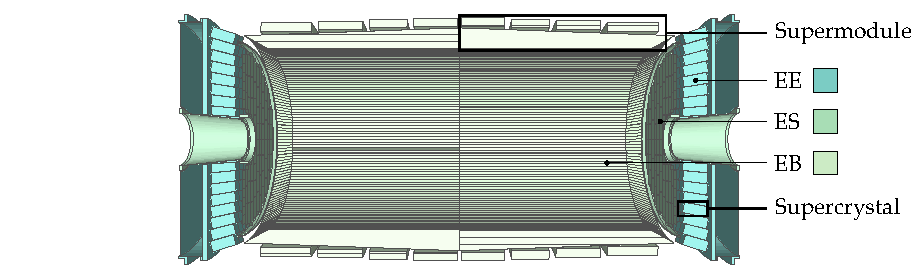
\includegraphics{diagrams/tikz/cms/annotated/cms_ecal.pdf}
    \caption{
        Front cross-sectional view of the \ECAL subdetector. Individual
        crystals are not shown, instead modules and supercrystals are
        displayed. The diagram was produced using the tools outlined in
        \cite{Sakuma:2013jqa}.
    }
    \label{fig:cms-ecal}
\end{figure}

The on-detector readout electronics for the \ECAL amplify and shape the signal
from the photodiodes and digitise at the bunch crossing rate of
${\SI{40}{MHz}}$. This data is buffered until an accept signal is received to
transfer the data to off-detector electronics for further processing. In
addition to this processing, the on-detector electronics run fast algorithms
on data from the ${5\times 5}$ clusters of crystals to aid in the accept
decision, detailed in Sec.~\ref{sec:hardware-trigger}.

The energy of a shower determined from photodiode signals is corrected to
reproduce the true energy of the particle initiating the shower. Several
factors result in the need for a correction factor, namely: an imperfect
clustering algorithm, energy loss from \brem, shower containment variations,
imperfections within the crystals, crystal-to-crystal variations, misalignment
of the crystals and limitations of the photodiodes. The reconstructed energy
of a shower, $E$, is given by
%
\begin{equation}
    E = G\mathcal{F}\sum_i c_i A_i\ ,
\end{equation}
%
where $G$ is the global absolute scale in converting GeV, determined from in
situ measurements of ${\PZ\ra\mu\mu\gamma}$. The function $\mathcal{F}$ is a
correction dependent on the type of particle; its position and momentum; and
the clustering algorithm used, determined from simulation validated by test
beam and in situ measurements of ${\PZ\ra ee}$ and ${\PZ\ra\mu\mu\gamma}$. The
product of $c_i$ --- the intercalibration coefficients obtained from
laboratory measurements, test beam precalibrations, comic ray measurements and
in situ ${\PW\ra e\nu}$ measurements, and ${\Ppizero\ra\gamma\gamma}$ and
${\eta\ra\gamma\gamma}$ mass reconstruction --- and $A_i$, the signal
amplitude, are summed over each clustered crystal labelled by $i$.

The corrected energy resolution of a supermodule is measured in a test beam by
fitting a gaussian function to the reconstructed energy distributions and
parameterised as
%
\begin{equation}
    \left(\frac{\sigma}{E}\right)^{2} = \left(\frac{S}{\sqrt{E}} \right)^{2}
    + \left( \frac{N}{E} \right)^{2} + C^2\ ,
\end{equation}
%
where $S$ is a stochastic tern, $N$ is a noise term and $C$ a constant term.
The total energy resolution ranges between {$1.50$--$0.35\%$} for
{$10$--$\SI{250}{GeV}$}, beyond which the constant term dominates.


\subsection{\HCAL}

The \HCAL is designed to provide full coverage of hadronic activity from a
proton-proton interaction, built from four distinct subdetectors, shown in
Fig.~\ref{fig:cms-hcal} found in the barrel (HB), endcaps (HE), beyond the
solenoid (HO) and far in the forward region (HF) \cite{Mans:1481837}. The HB
and HE subdetectors are sampling calorimeters, fully immersed within the
${\SI{3.8}{T}}$ field, with a brass absorber and plastic scintillator tiles in
a sampling ratio\footnote{The sampling ratio is the depth ratio of sampling to
absorbing elements.} of about $3:40$. The HB and HE are separated by a gap at
about $\SI{57}{\degree}$ designed to be non-projective with the interaction
point to avoid particles traversing an uninstrumented gap.

\begin{figure}[htbp]
    \centering
    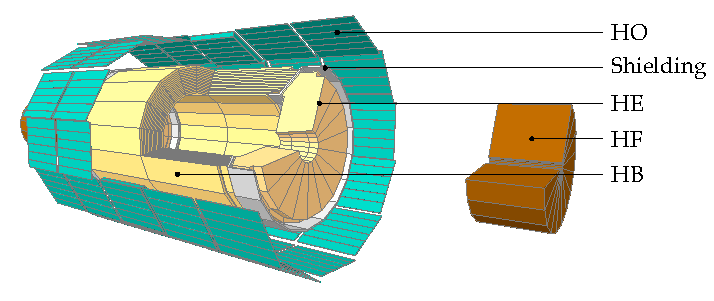
\includegraphics{diagrams/tikz/cms/annotated/cms_hcal.pdf}
    \caption{
        Front cross-sectional view of the four \HCAL subdetectors. The magnet
        between the HB and HO, along with the other subdetectors have been
        omitted. The HF is placed beyond the muon endcaps extending the
        coverage of the \HCAL in the forward region. The diagram was produced
        using the tools outlined in \cite{Sakuma:2013jqa}.
    }
    \label{fig:cms-hcal}
\end{figure}

The HB covers the central region up to $\aeta=1.4$ with a inner radius of
${\SI{1777}{mm}}$ and outer radius of ${\SI{2876.5}{mm}}$, made of two
half-barrels in $z$ of 18 identical wedges covering ${\SI{20}{\degree}}$ in
$\phi$ with further segmented into  ${\SI{5}{\degree}}$ sectors. The wedges
consist of towers: an alternating stack, parallel to the beam axis, of 17
active plastic scintillator tiles and brass plates, with the first and last
absorber replaced by steel for structural strength, forming a tower.
Constraints on the space  between the \ECAL and solenoid restricted the HB to
5.7 hadronic interaction lengths at ${\eta=0}$ and up to 9 at ${\eta=1.4}$,
necessitating the HO placed beyond the solenoid to improve the longitudinal
containment of hadronic showers. Scintillation photons are produced from the
interaction of hadronic showers with the active scintillation tile, collected
by wavelength shifting (WLS) fibres embedded within the plastic spliced to
clear fibres running along the tower. The optical signal is summed across the
depth of a tower in three groups: the first, the next 4 and the final 12
scintillator tiles (${\{1+4+12\}}$). The clear fibres are coupled to by
Silicon photomultiplers (SiPM). Full scintillator depth-segmentation would
allow hadronic shower discrimination, however, the segmentation is limited by
signal-to-noise, number of readout channels, power and cooling constraints.
Therefore, a balance of a three-depth configuration is in-place
\cite{Mans:1481837}.

The HE subdetector in the endcap provides coverage in the region
${1.3<\aeta<3.0}$, overlapping the HB for improved coverage across the
uninstrumented gap. The absorber-scintillator towers follow the same design as
the HB towers with wedges covering ${\SI{20}{\degree}}$ in $\phi$, segmented
to ${\SI{5}{\degree}}$ for towers in ${\aeta<1.74}$. The towers in
${\aeta>1.74}$ are instead segmented into ${\SI{10}{\degree}}$ to accommodate
the bending radius of the WLS fibres. The $\eta$ segmentation also increases
from ${0.087}$ for the towers at ${\aeta<1.74}$ to $0.09$--$0.35$ this $\eta$
range. The coarse azimuthal and polar segmentation allows for a finer depth
segmentation with configurations of four or five-depths in-place, grouped by
${\{1+2+3+5+7\}}$. The HE provides sufficient material interaction lengths
hence requires no outer calorimeter \cite{Mans:1481837}.

The HO consists of plastic scintillator tiles placed beyond the magnet to
catch energy leakage from the HB. Instead of brass, the solenoid and iron
return yoke act as the absorber extending the hadronic interaction lengths by
$2$--$3$. Two scintillator layers are placed at ${\eta=0}$, either side of a
${\SI{19.5}{cm}}$ thick piece of iron, where the interaction length of the HB
is the lowest. WLS fibres fed to SiPM detectors readout the signal from the
HO. The segmentation follows that of the muon system with ${\SI{30}{\degree}}$
wedges divides into ${\SI{5}{\degree}}$ sectors in $\phi$ to overlap with the
HB segmentation and five $\eta$ sectors up to ${\aeta=1.2}$. Partial plates
are placed around the cryogenics and power cables for the magnet.

High intensity radiation falls upon the HF, placed at ${|z|=\SI{11.2}{m}}$
downstream of the interaction point. Consequently, an alternative design of
steel absorbers embedded with radiation hard quartz fibres to produce
\cherenkov radiation from hadronic showers, detected by multi-anode
photomultiplier tubes \cite{Mans:1481837}. The steel absorbers are segmented
in $\phi$ by ${\SI{20}{\degree}}$ wedges subdivided into two
${\SI{10}{\degree}}$ sectors, apart from the two towers nearest to the beam
pipe which retain the ${\SI{20}{\degree}}$ segmentation. The steel absorber
towers are placed parallel to the beam axis with an $\eta$ segmentation of
approximately $0.175$, varying with $z$. The fibres also run parallel to the
beam axis placed ${\SI{5}{mm}}$ apart in an $x$--$y$ grid with alternating
long (full length of $10$ interaction lengths) and short (starting after $1.2$
interaction lengths). The two fibre lengths provide shower depth information
similarly to the depth segmentation in the HB and HE \cite{Abdullin2008HF}.

% Performance and calibrations?
%performance: Each subsystem has a laster and LED for monitoring and calibration. Since showers typically initiate in the ECAL the response and resolution of the CMS calo system depends on both the ECAL and HCAL. Corrections are determined from test beam studies. Resolution param by
%sigma/E = a/sqrt(E) oplus b
%From test beams of earlier HCAL designs: a = stochastic term and b constant term. a=0.847 +- 0.016, b=0.074 +- 0.008 for EB. EE is similar. HF has a=1.98 and b=0.09.
%
%calibrations: absolute energy scale, detector response and uniformity. Test beam of e, pi and mu. These are monitored with in situ measurements.
%performance: pions and electrons over 5-300 GeV. Low energy performance studied with muons. 


\subsection{Solenoid Magnet}

The muon identification requirement of the \CMS detector requires a large
bending power provided by the solenoid magnet with a field strength of
${\SI{3.8}{T}}$. Such a high field is obtained by a superconducting magnet,
shown in Fig.~\ref{fig:cms-magnet} maintained at operating temperatures by
superfluid helium cooling. To extend the bending power the return field is
focused by an iron return yoke spread throughout the muon chambers to about
${\SI{2}{T}}$.

\begin{figure}[htbp]
    \centering
    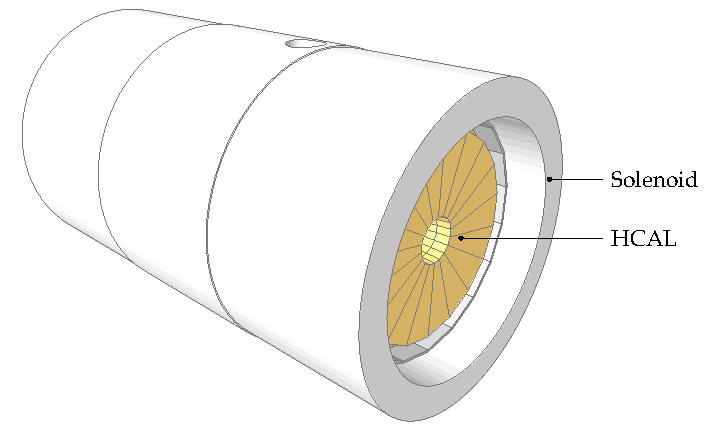
\includegraphics{diagrams/tikz/cms/annotated/cms_magnet.pdf}
    \caption{
        Isometric view of the solenoid and \HCAL with the muon chambers and
        HO removed. The diagram was produced using the tools outlined in
        \cite{Sakuma:2013jqa}.
    }
    \label{fig:cms-magnet}
\end{figure}


\subsection{Muon Chambers}

Muons from proton-proton collision, or secondary decays, travel through the
detector leaving tracks in the tracker and energy deposits in the calorimetry
system, however, most muons continue unscathed. The muon system is designed to
extend the 3-dimensional position measurements of these muons several metres
away from the interaction point. Three types of gaseous detectors are used
with the design driven by the large area to cover and different radiation
environments, particularly between the barrel and endcap.

The layout of the three gaseous detectors in the \CMS muon system is shown in
{Fig.~\ref{fig:cms-muon}}. In the barrel, anode wires centred in gas chambers,
known as a drift tubes (DT), collects the ionisation from passing charged
particles for 2-dimensional position measurements. DTs perform poorly in the
larger background and muon rate environment of the endcaps, hence cathode
stripe chambers (CSC) are in-place. A charged particle ionises the atoms of
the gas volume of a CSC with anode wires to collect the liberated electrons
and perpendicular copper cathode strips where a mirror charge is induced
allowing a full 3-dimensional position measurement. Resistive plate chambers
(RPC) accompany both the DTs and CSCs to provide fast responses with good
timing resolution at the cost of coarser positional resolution. The gas volume
within an RPC is ionised by charged particles with the liberated electrons
swept by an electric field induced from a large potential difference across
plastic tiles either side of the gas volume. The electrons are collected by
metal strips behind the plastic and the signal read out. The \CMS RPCs consist
of a double-gap separating ${\SI{2}{mm}}$ thick bakelite tiles by a
${\SI{2}{mm}}$ gas gap. 

\begin{figure}[htbp]
    \centering
    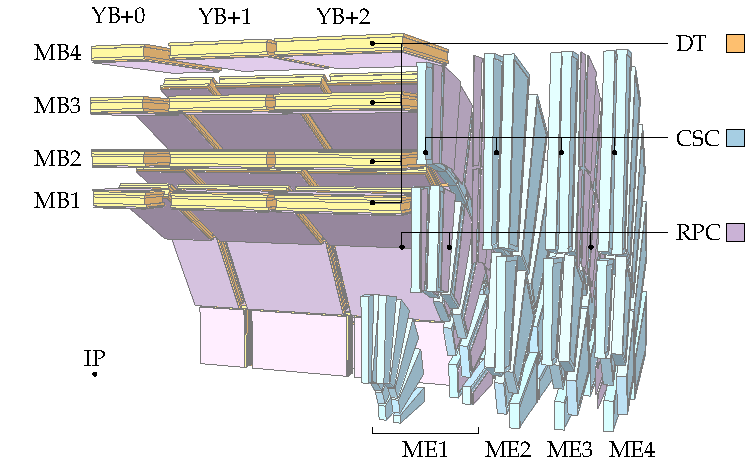
\includegraphics{diagrams/tikz/cms/annotated/cms_muon.pdf}
    \caption{
        Isometric view of the rear-top-right octant of the muon system,
        omitting the iron return yoke. The interaction point (IP) is shown in
        the lower left. The division of the muon system into stations (MB),
        wheels (YB) and disks (ME) are discussed in the text. The diagram was
        produced using the tools outlined in \cite{Sakuma:2013jqa}.
    }
    \label{fig:cms-muon}
\end{figure}

The muon barrel section (MB) cover ${\aeta<1.2}$ and consists of four concentric stations labelled MB1--MB4 position at about $4.0$, $4.9$, $5.9$ and ${\SI{7.0}{m}}$ away from the beam axis. Each station is subdivided into 12 sectors in $\phi$, with subsequent sectors overlapping to avoid uninstrumented gaps. Two partial sectors are placed around the magnet cryogenic lines and power cables. The MB is divided into five wheels along $\eta$ labelled $\mathrm{YB}-2$ to $\mathrm{YB}+2$. Stations MB1 and MB2 consist of two RPCs placed either side of a DT chamber whereas MB3 and MB4 have one RPC placed on the inside of a DT chamber. These DT chambers consist of four layers of drift tubes, known as a superlayer (SL). Two SLs have their anode oriented along the beam axis to measure the $r$-$\phi$ coordinates of muon tracks, $\mathrm{SL}_{\phi}$, and the third SL rotated by ${\SI{90}{\degree}}$ measures the $z$ coordinate (omitted in MB4), $\mathrm{SL}_{\theta}$. The SLs are separated by a honeycomb (HC) structure in the order: $\mathrm{SL}_{\phi}$, HC, $\mathrm{SL}_{\theta}$, $\mathrm{SL}_{\phi}$; where the final $\mathrm{SL}_{\phi}$ is omitted in MB4.

The muon endcaps (ME) enclose the solenoid both ends of the \CMS detector with
sufficient overlap with the barrel: $0.9<\aeta<2.4$. Both endcaps are divided
into four disks, labelled ME1--ME4, perpendicular to the beam axis, subdivided
into two concentric rings of 36 chambers (apart from ME2--ME4's innermost
rings with 18 chambers each). The chambers within a disk overlap to avoid
uninstrumented gaps. Each CSC is trapezoidal in shape with 6 gas gaps to
measure the $z$ position, cathode strips projecting radially outwards  to
measure the $\phi$ position and anode wires closely following the $\phi$
direction to measure the radial position from the beam axis. RPCs accompany
each CSC up to $\aeta=2.1$.

%- Readout
%- Calibrations
%- Alignment
    
\subsection{Hardware Trigger}\label{sec:hardware-trigger}

The ${\SI{40}{MHz}}$ bunch crossing frequency provided by the \LHC at 2016
luminosities yields on average 25 proton-proton interactions per crossing
leading to about 1 billion events per second. Storage capacities restrict full
detector archiving of about 100 crossings per second. Therefore, an online\footnote{Online refers to tasks or processes performed in real-time with strict timing constraints whilst data taking. Conversely, offline refers to processing after the storage of data without strict timing constraints.}
triggering system applies a rejection factor of the order of 1 in 10 thousand
with minimal impact to the broad physics program. This system is realised in
two-levels: the first level a hardware trigger (also known as the Level-1
trigger, \HWT) \cite{Bayatyan:706847,Tapper:1556311} with custom programmable
processors, and a second level a software trigger \cite{Sphicas:2002gg} using
general-purpose commercially available processors (discussed in
Sec.~\ref{sec:software-trigger}).

The detector data for each bunch crossing is held in on-detector buffers
whilst waiting on a decision from the \HWT to further process the crossing
with the software trigger. The \HWT processes up to 128 bunch crossings
simultaneously, allowing a total time of ${\SI{3.2}{\micro s}}$ on reaching a
decision. The allocated time includes data transit time to the electronics,
located in an adjacent cavern to the detector for radiation protection, which
reduces the total processing time to about ${\SI{1}{\micro s}}$. The \HWT is
sent a new bunch crossing to process every ${\SI{25}{ns}}$ and after the
allocated time a decision must be made, also every ${\SI{25}{ns}}$. These
restrictions prevent data fetching and result in most operations consisting of
simple arithmetic or querying memory in lookup tables\footnote{A lookup table
stores expensive computations in a pre-computed table for significant savings
in processing time and complexity.}. Furthermore, information from the tracker
and HO is omitted from the \HWT decision owing to their slow response. The
other subdetectors provide coarse information, to reduce processing time, and
are divided into the calorimeter and muon triggers with the candidates sent to
the global trigger for the final decision.

The \HWT decision is based on reconstruction of individual objects such as
photons, electrons, muons, jets, transverse energy sum or missing transverse
energy (\etmiss). The physics requirements can be summarised, with examples of
targeted physics, as follows:

\begin{enumerate}
    \item Triggering of events with a single lepton of ${\aeta<2.4}$ and
    ${\pt>\SI{40}{GeV}}$ with an efficiency above $95\%$ to target events with
    \PW decays.
    \item Dilepton triggers with the same kinematical requirements and an
    efficiency above $95\%$ to collect \PZ decays.
    \item Single photon and diphoton triggers with similar thresholds for
    processes involving a Higgs boson.
    \item \etmiss threshold about ${\SI{100}{GeV}}$ for sensitivity to new
    weakly interacting particles.
\end{enumerate}


\subsubsection{Calorimeter trigger}

\ECAL (EB and EE) and \HCAL (HB, HE and HF) signals are clustered into trigger
towers: ${5\times 5}$ arrays of crystals in the EB and EE; single physical
tower for the HE and HB up to ${\aeta=1.74}$ and twice the number of physical
towers in $\phi$ beyond this, whereby the energy of the physical tower is
divided equally between the trigger towers; and physical towers grouped into
pairs in $\phi$ and threes in $\eta$ for the HF. The transverse energy of each
trigger tower is determined by on-detector electronics and the result is sent
to the \HWT electronics along with flexible pass-fail information to, for
example, encode depth structure. This information is further processed with
each bunch crossing sent to one of ten processing nodes (with two redundant
nodes) to scan across the full ${\eta}$--${\phi}$ plane and identify physics
objects: jets, $\tau$s, electrons and photons; as well as calculating the
transverse energy sum and \etmiss. The processing nodes run concurrently with
a new bunch crossing occupying the first node upon completion of the previous
crossing. This is known as a time multiplexed system where the output must be
reassembled into the original bunch crossing order (de-multiplexed) for the
global trigger.


\subsubsection{Muon trigger}

The muon trigger system primarily consists of track finding from successive
chamber hits by a muon. This is divided into regional track finders using a
combination of the DTs and RPCs in the barrel (up to ${\aeta=0.8}$), CSCs and
DTs in the endcaps (from ${\aeta=1.25}$) and all three chambers in the overlap
region between the barrel and endcaps. Additionally, the system is tasked with
assigning hits to the correct bunch crossing, achieved by the high timing
precision of the RPCs and of the CSC's anode wire response. Timing is also
performed with the DTs, albeit with a poor resolution due to long drift times of
${\SI{400}{ns}}$. The tracks from these regional triggers is sent to the
global muon trigger to merge and remove duplicate muon candidates, along with
combining the isolation information from the calorimeter trigger, and finally
sorts the muons for the global trigger.


\subsubsection{Global trigger}

The trigger objects and variables received from the calorimeter and muon
triggers is collected at the global trigger for synchronisation and
correlation of relevant trigger candidates. The union of a set of requirements
on the trigger objects is determined and forms the basis of the \HWT decision.
However, evolving conditions and the collection of events from high
cross-sectional processes requires the global trigger to reject random events
to reduce the trigger rate. This process is known as prescaling and reduces
the trigger efficiency by the prescale factor: e.g. a prescale factor of 10
will accept 1 out of 10 events regardless of decision formed from the trigger
candidates resulting in a rate reduction of a factor of 10 and a drop
efficiency of $90\%$. After the prescaling is applied the \HWT decision is
communicated to the data buffers to discard or transmit the bunch crossing to
the software trigger.


\subsection{Software Trigger}\label{sec:software-trigger}

The software trigger (also known as the high-level trigger, \SWT) accepts the
full detector granularity and all subdetector information from the on-detector
readout. All bunch crossings filtered by the \HWT are distributed among
processing nodes in a processor farm, each node running a copy of the software
code to reconstruct and reject events. To meet the timing constraint, the \SWT
performs a partial reconstruction of the event at first, guided by the trigger
objects from the \HWT, gradually performing the full reconstruction until the
event fails the trigger criteria. Furthermore, the \SWT must be efficient at
selecting physics objects of interest and inclusive to avoid rejecting exotic
physics. Therefore, the \SWT reconstruction is closely aligned with offline
reconstruction (discussed in Chap.~\ref{chap:reconstruction}). However,
calibrations and other run conditions available for offline analysis cannot be
used. After accepting an event, the data is archived and made readily available
for further analysis by the computing grid.


\subsection{Worldwide \LHC Computing Grid (\WLCG)}

Despite the data reduction achieved by the \CMS trigger system, a vast amount
of data was accepted and requires prompt full reconstruction with possible
revisions in light of improved object reconstruction, calibrations or code
errors. Moreover, simulations of proton-proton collisions within the \SM and
possible \BSM physics, including a simulation of the detector, the trigger and
pileup with full reconstruction demands a significant amount of processing
power. To achieve this the \WLCG was established \cite{Bird:1695401}. The
\WLCG is a highly distributed computing cluster divided into tiers situated
at: the main \CERN site, national laboratories and Universities worldwide. The
computing  provides the resources required for data reconstruction and
simulations, and supports in the design, evaluation, construction and
calibration of the detector and future upgrades.


\section{Summary}

The \LHC provides proton-proton bunch crossings at a rate of ${\SI{40}{MHz}}$,
a centre-of-mass energy of ${\SI{13}{TeV}}$, and the \CMS detector centred on
one of these crossings. The \CMS detector is designed to detect and
reconstruct the position and momenta of outgoing particles from the collisions
whilst mitigating backgrounds such as noise and pileup, and optimising the
geometry and readout channels with modern technology. The main feature is a
${\SI{3.8}{T}}$ solenoid enclosing the silicon tracker and calorimetry with an
outer muon system. A two-level trigger system reduces the data output by
selecting events of interest for a manageable output rate for archiving.
The immense processing power required for further analysis of the data and
production of simulations is mediated by the \WLCG.
        \chapter{Event reconstruction}\label{chap:reconstruction}

%\chapterquote{}{}

\section{Introduction}

The apparent simplicity --- hits from ionising particles and energy deposits
from particle showers --- and the detector granularity of \CMS allows the
reconstruction and identification of muons, electrons and photons, and charged
and neutral hadrons. Instead of simply detecting, reconstructing and
identifying particles with their respective dedicated system an improvement is
made from correlating elements from all detector layers with an attempt to
distinguish each individual particle by a technique known as particle flow (PF).

The initial step in reconstruction, prior to the PF method, consists of
forming charged particle tracks from hits in the silicon tracker, tracks in
the muon chambers and calorimeter clusters from energy deposits in the
calorimetry system. The basic building blocks form the input into the PF
algorithm which attempts to link the various blocks into a coherent picture of
a particle candidate. For example, tracks are linked to an \ECAL deposit to
form an electron candidate with further linking to \ECAL deposits consistent
with Bremsstrahlung photons from the electron, which may undergo conversion
resulting in displaced electrons tracks also linked to the primary electron.
Furthermore, the reconstruction of all particles results in a simple \ptmiss
calculation from the negative vector sum of all particle momenta.

This chapter will describe in detail the process of tracking, clustering and
the PF method in the full reconstruction of a proton-proton interaction.


\section{Tracking}

Charged particles originating from the interaction point travel outward
through the magnetic field in helical trajectories. The hits in the silicon
tracker are reconstructed into the track by a fitting procedure known as the
combinatorial track finder. Hits are formed within the pixel tracker by
clustering deposits, above a certain threshold, in adjacent pixels. The
position of the hit for single pixel clusters is taken at the centre of the
pixel while multi-pixel clusters have a charge-weighted position, correcting
for the drift of electrons in the magnetic field. A more sophisticated,
albeit, computationally demanding method is used for the final track fit which
involves a $\chi^2$-fit of expected charge deposits from a large number of
simulated particles through the pixels to the observed charge deposit,
accounting for pixel deterioration. Strip tracker hits are formed from
clusters of adjacent strips with charge deposits exceeding a noise-level. The
hit position is determined from a charge-weighted average of the cluster,
correcting for the electron drift in the magnetic field and known
inefficiencies with the charge collection. All hits have an associated
uncertainty propagated to the track fitting procedure~\cite{Chatrchyan:1704291}.

The combinatorial track finder involves a series of Kalman filters (KF)
\cite{Kalman:1960} --- a recursive parameter estimator. A Kalman filter starts
with an initial state (a seed), typically from a guess or estimation,
and iterates across measurements updating the initial state parameters by
comparing the prediction to the observations. For track fitting, the fit is
performed to five parameters which describe points along a helical track, known
as the perigee parameterisation:
%
\begin{equation}
    \left( \frac{q}{\pt}, x_t, y_t, \theta_t, \phi_t \right)\ \,
\end{equation}
%
where $q/\pt$ is the ratio of the charge to track transverse momentum to give
the signed curvature scale of the trajectory. The parameters $x_t$ and $y_t$
are the distances from the interaction point to a point along the trajectory
in the $\vec{x}_t$ and $\vec{y}_t$ axis, shown in Fig.~\ref{fig:kf_parameters}
along with the definitions of the angles $\theta_t$ and $\phi_t$.

\begin{figure}
    \centering
    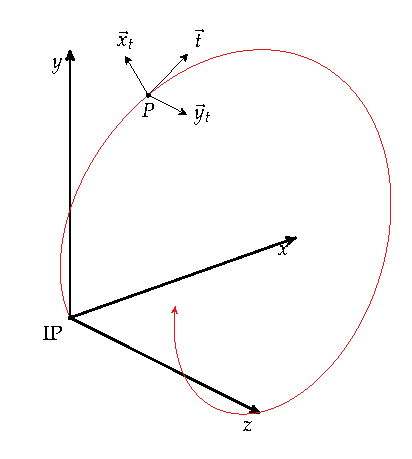
\includegraphics{diagrams/tikz/kf_parameters/kf_parameters.pdf}
    \caption{
        Diagram of a track (shown in red) from the interaction point (IP) with
        the conventional \CMS coordinate system as well as a local coordinate
        system along the trajectory, an example of which is shown at point $P$
        where $\vec{t}$ is the tangential vector, $\vec{x}_{t}$ is
        perpendicular to both the z-axis and $\vec{t}$ and $\vec{y}_{t}$ is
        the remaining vector to create a right-handed coordinate system. The
        angle between the $x$-axis and the projection of ${\vec{t}}$ onto the
        $x$-$y$ plane is $\phi_t$. Similarly, the angle between the $y$-axis
        and the projection of ${\vec{t}}$ onto the $y$-$z$ plane is $\theta_t$.
    }
    \label{fig:kf_parameters}
\end{figure}

The trajectory building with a Kalman filter starts with the seed generation
stage by combining a set of pixel hits, where the resolution is  a setthe
greatest and occupancy the lowest. Each iteration of the Kalman filter extends
to the next tracker layer where each hit candidate, within a $\chi^2$ window,
is kept to form independent track candidates. Fake tracks will typically have
a layer where no hits are within the window and can be dropped. Further checks
are performed on the consistency of hits with the \pt of the track and from
vertex constraints. Finally, a cleaning process assigns unique tracks to a
seed and vice versa. After determining the full set of tracks, the Kalman
filter procedure is repeated with the precise hit reconstruction, accounting
for inter-layer material and field inhomogeneities, with inflated
uncertainties to avoid biasing the initial result. Furthermore, the Kalman
filter is repeated, seeded by hits from the outermost layer iterating inwards.
The best fit tracks are taken from an average of the Kalman filter starting
from the inner layers and the reverse.

The trajectory building is performed ten times with different seeds to target
various classes of tracks with hits associated with candidate tracks removed
from subsequent iterations:
\begin{itemize}
    \item Prompt and high \pt tracks, and $b$-hadron decays are target by the
    first three iterations, seeded by three hits in the pixel detector with
    constraints on the track \pt and distance of nearest approach to the beam axis.
    \item The fourth and fifth iteration target tracks with one or two missing
    hits in the pixel detector as a result of particle interactions and
    decays, or detector inefficiencies. These are seeded by two pixel hits or
    a combination of three pixel and strips hits.
    \item The next two iterations are seeded by strip hits to target displaced tracks.
    \item The eighth iteration targets high \pt jets with merged constituent
    tracks, seeded by pairs of hits in the pixel and strips with the initial
    track compatible with a high energy calorimeter deposit.
    \item The final two iterations are designed to track muons missed by prior
    iterations by using information from the muon chambers to determine the seeds.
\end{itemize}
After all iterations are complete a full set of tracks within the tracker
volume are defined, known as inner tracks.


\subsection{Electron tracking}

Electron tracks may be missed by the combinatorial track finder as a result of
significant Bremsstrahlung and high energy photon emission. To recover these
tracks another fitting procedure is performed, based on a gaussian-sum filter
(GSF). The GSF method models hits by a weighted sum of gaussian distributions
for a more accurate representation of hits with sudden and substantial
radiative losses. The results of the expectation fit to the observed hits is
fed into a boosted decision tree\footnote{A boosted decision tree is a form of
supervised artificial learning with an output from a weighted linear sum of
many decision trees, determined by optimising a function of the truth and
prediction with a regularisation term to penalise tree depth.} (BDT) to
optimise electron track reconstruction efficiency while minimising fake
tracks. This procedure is also effective at tracking electron-positron pairs
from tracker converted photons.


\subsection{Muon tracking}\label{subsec:muon-tracking}

A track fitting procedure is performed with hits in the muon chambers to form
muon track candidates. Various quality muons are defined based on the inputs
and results of the track fitting:

\begin{itemize}
    \item \textbf{standalone muon:} track fitting seeds are formed of track
    segments from hits within the DT or CSC detectors. The fit itself uses
    hits within all muon chambers.
    \item \textbf{global muon:} a standalone muon track matched to an inner
    track.
    \item \textbf{tracker muon:} one muon segment matched to a unique inner
    track with requirements on the muon's momentum and its compatibility with
    an origin at the beam axis.
\end{itemize}


\section{Vertex reconstruction}\label{sec:vertex-reco}

The conditions provided by the \LHC during 2016 data-taking yielded on average
about 25 proton-proton interactions per bunch crossing. Since the triggering
system selects about 1 in 100 thousand crossing at most one of these
interaction points are of interest per event, known as the primary vertex. The
other vertices are classified as pileup which result in additional particles
leading to misreconstruction of the primary event. Therefore, the reconstruction
of these vertices is critical in mitigating the impact of pileup interactions,
particularly in determining the \ptmiss of the primary event.

The vertex reconstruction is performed by a fit to a selection of tracks. The
collection of tracks are selected by their track quality parameters
(sufficient number of hits and a satisfactory track fit $\chi^2$) and
consistency with the beam spot, a 3-dimensional profile of the luminous
region determined from an average over multiple bunch crossings. From these
track collections a set of vertex seeds are found by searching for convergence
points of multiple tracks \cite{Speer:927395}. These seeds initialises the
adaptive vertex fitter \cite{Fruhwirth:1027031}, a similar procedure to the
Kalman filter although all tracks are considered in turn weighted by the
compatibility of the track's nearest approach to the vertex seed. This is
followed by updating the vertex position from a method of least squares to the
weighted tracks. This procedure is iterated until convergence resulting in a
collection of vertex candidates. The primary vertex is selected from this
collection by the greatest $\sum \pt^2$ over all outgoing tracks
\cite{Sirunyan:2017ulk}.


\section{Calorimeter clustering}

A clustering algorithm groups energy deposits within the calorimeter towers to
encapsulate the whole extend of a particle shower, or multiple overlapping
showers. These clusters are sent to the PF algorithm to link the cluster with
a track, or multiple tracks. The clustering is performed separately in the
ECAL barrel and endcaps, HCAL barrel and endcaps, and the two preshower
layers. No clustering is performed in the HF since forward jets typically have
large momenta and hence collimated showers. Seeds initialise the clustering
and are identified as cells with an energy above a threshold and greater than
the nearest neighbouring cells. Topological clusters are formed by continually
merging neighbouring cells, with an energy twice the noise level, into the
cluster. Individual clusters within a topologial cluster are distinguished by
a gaussian-mixture model: a topological cluster in $M$ cells arise from $N$
gaussian energy deposits. The deposits are parameterised by the amplitude of
the $i$-enumerated gaussian, $A_i$; the position of the gaussian centre in
$\eta$-$\phi$, $\vec{\mu}_i$; and the width $\sigma$ of the gaussian, fixed to
values assigned for each calorimeter system. The initial values are taken from
the cell seeding the topological cluster and an expected energy fraction
measured in cell $j$ is determined from
%
\begin{equation}
    f_{ji} = \frac{A_i\exp\left(-(\vec{c}_i-\vec{\mu}_i)^2/(2\sigma^2)\right)}{\sum_{k=1}^{N}\exp\left(-(\vec{c}_j-\vec{\mu}_k)^2/(2\sigma^2)\right)} ,
\end{equation}
%
where $\vec{c}_i$ is the position of element $i$. The parameters are estimated
from an analytical maximum likelihood fit with
%
\begin{equation}
    A_i & = \sum_{j=1}^{M} f_{ji}E_j
\end{equation}
%
and
%
\begin{equation}
    \vec{\mu}_i & = \sum_{j=1}^{M} f_{ji}E_j\vec{c}_j\ ,
\end{equation}
%
where $E_j$ is the energy deposited in cell $j$. This fit is iterated until
convergence and the position and energy of the gaussian functions are taken as
the cluster parameters.

The energy of the clusters are calibrated to accurately reflect the true
energy deposited. The calibrations are applied independently to
electromagnetic and hadronic deposits, reflecting the difference in the
corresponding showers. Calibrations are determined from test beam data,
radioactive sources, cosmic ray measurements, in situ collision data and
simulated events.


\section{The particle flow algorithm}

The PF algorithm attempts to resolve all particles from the interaction point
by exploiting the high granularity of the \CMS detector. The algorithm must
deal with particle interactions within the detector leading to crooked tracks
(bent at a `kink') and secondary particles. Furthermore, to avoid a quadratic
computation with the number of particles only the nearest neighbouring PF
blocks in $\eta$-$\phi$ are considered as candidates in the linking algorithm.

The linking of inner tracks to muon tracks has been discussed in
{Sec.~\ref{subsec:muon-tracking}}. Calorimeter clusters are linked to inner
tracks by extrapolating the track to the \ECAL or \HCAL and a link formed if
these positions lie within a topological cluster's cells, allowing sufficient
margins to account for gaps in calorimeter coverage, shower profile
uncertainties and multiple scattering. A link distance quantifies the distance
between the extrapolated track position and the cluster position in
$\eta$-$\phi$ with the link of minimum distance kept. Bremsstrahlung photons
are linked to electron GSF tracks if tangents, at each tracker layer, to the
track are consistent with \ECAL clusters. A dedicated conversion finder
creates a link between two tracks and a photon if the track are compatible
with the characteristics of a photon conversion. Clusters are linked together
(preshower to \ECAL and \ECAL to \HCAL) if the more granular calorimeter
cluster is within the less granular calorimeter cluster, retaining the link
forming the minimum distance between the two clusters. Finally, tracks are
linked together through a common secondary vertex, attributed to
nuclear-interactions. These tracks must contain at least three tracks: one
incoming from the primary vertex and at least two outgoing, or at least three
outgoing. All links are formed and the subsequent part of the PF algorithm
recovers inefficiencies and removes fake particle candidates by targeting
particular particle classes, as follows.

    
\subsection{Muons}

Global muons are classified as isolated to avoid the misidentification of
charged hadrons, whereby the total energy in a cone of radius ${\Delta
R=\sqrt{\Delta\eta^2+\Delta\phi^2}=0.3}$ around the muon candidate must not
exceed $10\%$ of the muon \pt:
%
\begin{equation}
    I_{\mathrm{track,calo}} = \frac{1}{\pt}\Biggl(\bigg|\sum_{\substack{i\in \mathrm{tracks}\\\Delta R<0.3}} \vec{p}_{\mathrm{T},i}\bigg| + \sum_{\substack{j\in \mathrm{clusters}\\\Delta R<0.3}}E_{\mathrm{T}}\Biggr) < 0.1\ ,
\end{equation}
%
where $I_{\mathrm{track,calo}}$ is known as the track-calorimeter isolation,
$i$ sums the transverse momenta of all tracks within $\Delta R=0.3$ and $j$
sums the transverse energies of all clusters within $\Delta R=0.3$.
Non-isolated muons are also identified without the isolation requirement,
however, inner tracks must match at least three track segments in the muon
detectors or calorimeter clusters compatible with the muon hypothesis to avoid
high \pt charged hardon misidentification.

The \pt of PF muon candidates is reconstructed from the tracker for
${\pt<\SI{200}{GeV}}$, otherwise the \pt is taken from the track fit resulting
in the lowest $\chi^2$ from the following combinations of information: tracker
only, tracker and the first muon detector plane, global muons, and global muons
without high occupancy muon detector planes. After all PF muon candidates are
identified and reconstructed the associated PF blocks are removed from further
candidate identification. Note that under certain conditions charged hadrons
may later be revised as muons.


\subsection{Electrons and isolated photons}

Electron and isolated photon reconstruction must collect and associate
Bremsstrahlung photons and electrons from photon conversions to accurately
measure the true energy of these particles. These secondary particles are
associated to a seed candidate: an \ECAL supercluster above a transverse
energy threshold of ${\SI{10}{GeV}}$ with no GSF track link for photons, or
GSF tracks associated to \ECAL clusters with fewer than three additional
linked tracks. Both classes of candidates must not have \HCAL clusters within
${\Delta R=0.15}$ of the candidate with an energy deposit exceeding $10\%$ of
the supercluster energy. The assigned energy of the candidate is determined
from the sum of all energy deposits linked to the seed, this includes
Bremsstrahlung photons at tangents to GSF tracks at tracker layers and GSF
tracks found by the conversion finder. This energy is calibrated and taken as
the final energy for isolated photon candidates. Electron candidate's energy
is determined from a combination of the calibrated \ECAL energy and GSF track
momentum.

To further reduce misreconstruction the candidates must pass additional
criteria. A BDT is trained separately for the barrel and endcaps, and for
isolated and non-isolated electrons with a requirement placed on the output
determined by the following input features: energy radiated from the GSF
track, distance between the GSF track extrapolation and the \ECAL seeding
cluster, ratio of the \HCAL to \ECAL energy, KF and GSF track $\chi^2$ and the
number of hits in the tracker. Photons, on the other hand, are required to be
isolated from other tracks, calorimeter clusters and have \HCAL to \ECAL
energy ratios consistent with typical photon showers.

Finally, as with muons, the PF blocks associated with the electron and
isolated photon candidates are removed from further processing.


\subsection{Hadrons and non-isolated photons}

The remnants of jet fragmentation and hadronisation with the subsequent decay
of heavy hadrons include: charged hadrons such as $\Ppipm$, $\Pkpm$ and
protons; neutral hadrons such as $\Pklzero$ and neturons; non-isolated photons
typically from $\Ppizero$ decays; and rarely additional muons from early
charged hadron decays. Discrimination of hadrons, other than charged and
neutral, is difficult with high misidentification rates, therefore, the PF
algorithm makes no attempt at this distinction.

From the remaining PF blocks, all \ECAL clusters within the tracker acceptance
(${\aeta<2.4}$) with no linked tracks are considered as photons. Similarly,
\HCAL clusters with the same acceptance with no linked tracks are treated as
neutral hadrons. This assumption holds well within the tracker acceptance where
charged and neutral hadrons are distinguishable and $25\%$ of the jet's energy
is deposited in the \ECAL as photons while only $3\%$ as neutral hadrons
($1\%$ for $\tau$-lepton decays as a result of Cabibbo-suppression). However,
beyond ${\aeta=2.4}$ up to the \ECAL acceptance (${\aeta<3.0}$) the precedence
to photons leads to a high misidentification rate of charged and neutral
hadrons, which can account for $25\%$ of the jet's energy deposited in the
\ECAL. Instead, \ECAL clusters linked to \HCAL clusters are assigned as hadron
showers with an unknown charge, while \ECAL clusters without this link are
considered photons. Beyond ${\aeta=3.0}$, within the HF, electromagnetic and
hadronic activity are identified by exploiting depth information and lateral
shower profiles by comparing $3\times 3$ to $5\times 5$ clusters.

Misidentification and misreconstruction may leave inconsistencies in the
calibrated calorimetric energy and tracker momenta for charged hadrons. These
are dealt by reassigning the identification or refining the reconstruction,
since the excess infers the presence of photons or neutral hadrons. If the
calibrated cluster energy $E_T$ is in excess, by $\delta_T$, of the sum of
linked track momenta, $|\sum \vec{p}_T|$, where ${\SI{500}{MeV}<\delta_T<E_T}$
then $\delta_T$ is attributed to a photon. If $\delta_T>E_T$, the $E_T$
deposit is revised as a photon and $\delta_T$ is assigned to a neutral hadron.
If the excess is small but inconsistent with the energy resolution
$\sigma(E_T)$, ${\sigma(E_T)<\delta_T<\SI{500}{MeV}}$, a $\chi^2$ fit to the
tracker and calorimeter information is performed to refine the energy of the
charged hadron. Finally, in the rare case where the track momenta are in
excess of $E_T$, i.e. $\delta_T<0$, a relaxed search for muon candidates is
performed. Any remaining excess is associated to misreconstructed tracks with
a momentum resolution greater than ${\SI{1}{GeV}}$. The leading\footnote{Leading refers to the candidate in a collection with the largest \pt.} misreconstructed track candidate is repeatedly removed until no excess or no
candidates remain.

Displaced tracks within the tracker volume predominantly from nuclear
interactions are yet to be identified. These involve secondary
charged particle tracks linked to a secondary vertex. The charged particles
are replaced by a single charged hadron, conserving energy and momentum, with
a mass of a charged pion. If a primary charged particle track exists, with a
well-defined momentum, then any deficit in the outgoing energy is attributed
to undetected secondary particles and the energy of the primary charged
hadron is updated to account for these particles.


\subsection{Jets}

The fragmentation and hadronisation of outgoing quarks form a cone of hadrons
known as a jet. The anti-\kt algorithm \cite{Cacciari:2008gp,Cacciari2012}
discussed in Sec.~\ref{sec:theory} clusters PF candidates into cones of
radius $R=0.4$ in the $\eta$-$\phi$ plane.  The minimum clustering threshold
is set to $\SI{15}{GeV}$, below which jets are unreliable at mirroring the
underlying physics. Seeding jets by PF candidates improves the energy
resolution by complimentary tracker measurements for charged hadrons affected
by the poorer hadron calorimeter resolution. However, as with any other jet
seed, neutrinos from hadron decays within  the jet are not accountable.


\subsection{Missing transverse momentum}

The PF method allows a simple calculation of the uncorrected (or raw) \ptmiss
from:
%
\begin{equation}
    \vec{p}_{\mathrm{T,raw}}^{\mathrm{miss}} = - \sum_{i} \vec{p}_{\mathrm{T},i}\ ,
\end{equation}
%
where $i$ sums over the PF candidates. However, residual misidentification and
misreconstruction can lead to a large \ptmiss similar to new physics
processes. To control the artificially large \ptmiss all particles with a
significant correlation with the direction and magnitude of the \ptmiss are
selected. The particles are typically high \pt muons and their identification
and reconstruction revised as follows:
%
\begin{itemize}
    \item \textbf{Genuine cosmic ray muons} in coincidence with an \LHC beam
    crossing, positioned further than ${\SI{1}{cm}}$ from the beam axis, are
    removed from the PF candidate collection if this leads to a reduction in
    the \ptmiss of at least a half. Semi-leptonic decays of $b$-hadrons are
    protected as their removal would increase the \ptmiss.
    \item \textbf{Severely misreconstructed muon momentum} as a result of
    wrong track association, steel yoke interactions, in-flight decay or
    significant synchrotron radiation. Here, the reconstruction of muons with
    ${\pt>\SI{20}{GeV}}$ is reviewed and the \pt updated if it leads to a
    reduction in the \ptmiss by at least a half.
    \item \textbf{Particles misidentified as muons} typically from
    charged-hadronic punch-through into the muon systems. In this case, neutral
    hadron deposits within the calorimeters are wrongfully included as
    independent particles leading to a double-counting of the charged hadron
    as a muon and a neutral hadron. Provided that the \ptmiss is reduced by a
    half and the muon momentum and neutral hadron energies are larger than
    ${\SI{100}{GeV}}$, then the neutral hadron is removed and the muon is
    revised as a charged hadron.
    \item \textbf{Muon and neutral hadron overlap} with similar energies which
    are misidentified as a charged hadron. The charged hadron is converted
    into a muon and a neutral hadron if the associated \ptmiss is reduced by a
    half.
\end{itemize}
%
After these revisions the \ptmiss is updated and the approach validated with
in situ measurements and studies in simulated events which show minimal impact
on processes with real \ptmiss, such as the pair-production of $t\bar{t}$.


\section{Summary}

The \CMS software reconstruction incorporates the whole detector, correlating
detector elements to improve particle identification and reconstruction with an
attempt to reconstruct all detectable particles in a technique known as
particle flow. The PF algorithm starts from two basic building blocks: tracks
and clusters. Tracks are formed from a series of Kalman filters applied to
hits: charge deposits within the tracks. An alternative GSF track finder
attempts to reconstruct the tracks of electrons subject to radiative losses.
Vertex reconstruction is performed from a fit to high-quality track candidates
consistent with the beam spot and the primary interaction point identified as
the vertex with the greatest $\sum \pt^2$ over outgoing tracks. On the other
hand, clusters are formed from energy deposits within calorimeter cells,
grouped and refined by a gaussian-mixture model. 

The PF algorithm links the building blocks (tracks and clusters) to form a
coherent picture of each individual particle with complementary measurements
from the various subdetectors. Muon candidates have links between inner and
muon chamber tracks. Electron and isolated photon candidates are formed from
\ECAL clusters, linked to GSF tracks for electrons, with further linking to
clusters consistent with Bremsstrahlung photons or GSF tracks compatible with
photon conversions. Hadrons and non-isolated photons have possible links
between tracks, \HCAL and \ECAL clusters. Further refinement is performed on
irregular candidates. After all PF candidates are determined jets are
clustered from all candidates with the anti-\kt algorithm and the \ptmiss
determined from a negative sum over all candidate $\vec{p}_{\mathrm{T}}$
with possible identification revisions to avoid large spurious
\ptmiss.
        \chapter{Event Selection and Categorisation}
\label{chap:analysis}

%\chapterquote{}{}
% \cite{Alwall:2014hca}.

\section{Introduction}

The measurement of the \IZinv width requires the collection of \IZvvj signal events with the key signature of jets recoiling against an invisible system, also known as \metplusjets. The \IDYllj process is used as a reference to extract the invisible width, under the assumption of a purely \SM \IZll interaction. In addition, samples of \IWlvj provide a data-driven estimate of large backgrounds with a similar signature to the signal. A combination of the large QCD multijet cross-section and inherent jet misreconstruction leads to additional backgrounds and the need of a sideband\footnote{A sideband is an independent set of events to a region obtained by inverting or somehow altering a requirement which defined the original region.} enriched with QCD multijet events for a data-driven estimate of this background.

This chapters details the process of data collection and reduction to target specific processes in various categories required for this analysis. Included is the detail of particle identification refinement from the PF algorithm results for an improved signal acceptance whilst maintaining a high background rejection.

\section{Samples}

\subsection{Data collection}

Detector measurements associated to a proton-proton bunch crossing are stored by various sets of \SWT requirements, known as \SWT paths. The dataset under consideration was collected during 2016 with proton-proton collisions at a centre-of-mass energy of ${\SI{13}{TeV}}$. Issues during detector live-time, such as problems with a particular subdetector or beam conditions, requires the rejection of problematic data resulting in a dataset with an integrated luminosity of ${\SI{35.9}{fb^{-1}}}$.

The relevant process can be classified into events with missing transverse momentum or more than one lepton. Events with a significant missing transverse momentum are selected by the \SWT paths requiring two conditions or a third to be satisfied. The first is
%
\begin{equation}\label{eq:hlt_met_trig_selection1}
    \ptmissnomu = \bigg| -\sum_{i\not\in\mathrm{muons}} \vec{p}_{\mathrm{T}} \bigg| \ge \ptmissthresh\ ,
\end{equation}
%
where the sum is over all PF candidates apart from muons and \ptmissthresh is a particular threshold. The muons act as invisible particles for \ptmissnomu hence this collects \IZvv, \IWmv and \IDYmm events. The second condition is
%
\begin{equation}
    p_{\mathrm{T,had}}^{\mathrm{miss}} = \bigg| -\sum_{i\in\mathrm{jets}} \vec{p}_{\mathrm{T}} \bigg| \ge \ptmissthresh\ ,
\end{equation}
%
summed over all PF jets passing the tight jet identification selection with ${\pt>\SI{20}{GeV}}$ and no muon candidates. This selection is similar to Eq.~\ref{eq:hlt_met_trig_selection1}, however, the combination of both maintains a trigger rate for lower \ptmissthresh  thresholds by removing events with inconsistent visible (excluding muons) and hadronic recoils, primarily due to misreconstructed soft (${\pt<\SI{20}{GeV}}$) hadronic activity. The threshold \ptmissthresh varies from {$90$--$\SI{120}{GeV}$} depending on the \LHC beam conditions to avoid prescaling. The third condition recovers small inefficiencies by applying the selection
%
\begin{equation}
    \ptmiss = \bigg| -\sum_{i\in\mathrm{PF}} \vec{p}_{\mathrm{T}} \bigg| \ge \SI{170}{GeV}\ ,
\end{equation}
%
summed over all PF candidates, with various beam halo or \HCAL noise cleaning requirements (discussed in Sec.~\ref{sec:baseline-selection}) to maintain this threshold as beam conditions change.

A complementary trigger path collects events with at least one muon rather than the momentum imbalance of an event. Events pass the trigger requirement if there exists a global or tracker muon with ${\pt>\SI{24}{GeV}}$ which is isolated from other activity (total energy within a cone of $\Delta R=0.3$ is below $9\%$ relative to the muon \pt). To collect events with at least one electron an alternative trigger path is used with the requirement of at least one GSF electron passing a tight identification selection and a ${\pt>\SI{27}{GeV}}$. Both lepton trigger thresholds are driven by a goal to maintain data collection efficiency and control trigger rates.


\subsection{Simulation}

A vast array of simulated proton-proton collisions attempt to fully replicate the events selected as signal candidates, including backgrounds with similar experimental signatures to the signal. Vector boson production; namely \IZvv, \IWlv, \IDYll and prompt photon; in association with jets, \IVj, are produced with the matrix element (ME) event generator \MADGRAPH \cite{Frederix:2018nkq} with restricted boson decays and Feynman diagrams up to $\mathcal{O}(\alpha^2\alpha_s^2)$, hereby known as next-to-leading order (NLO) in the strong coupling constant. The production is split into boson \pt regions to populate the low cross-section high-\pt regions. These generated events are coupled to the \PYTHIA package \cite{Sjostrand:2014zea} to mediate the parton showering (PS), hadronisation and particle decays with the \CUET underlying event description \cite{Khachatryan:2015pea}. Double-counting of jet multiplicity final states with the ME and PS is removed by the FXFX \cite{Frederix:2012ps} matching and merging technique. Another set of processes similar to \IDYll are generated where, in turn, the \PZ and \Pgstar interactions are turned off to model the \PZ, \Pgstar and interference terms of the \IDYll process. Furthermore, the processes involving a \Pgstar have an invariant mass cut-off below ${\SI{50}{GeV}}$ to avoid the large cross-section away from the \PZ peak.

Minor background processes include the pure QCD interactions between partons forming a multijet final state with jet misreconstruction leading to spurious \ptmiss, faking the signal signature. The QCD multijet process is produced at leading order (LO) accuracy in the strong coupling constant by the \PYTHIA package, split by the interaction scale $Q^2$ to populate the low cross-section regions. Top production leads to real \ptmiss with zero, one or two leptons in the final state with the pair production, \Ittj, produced using a similar technique as the \IVj processes, albeit inclusive in \pt, and single top production --- via the $s$-channel, $t$-channel or associated \PW production --- are produced at NLO by a various combination of the \MADGRAPH, \MADSPIN \cite{Artoisenet:2012st}, \PYTHIA and \POWHEG \cite{Alioli:2010xd,Alioli:2009je,Re:2010bp} packages. Diboson processes (combination of \PZ, \PW and prompt \Pgamma from the hard scatter) may have a similar signature to the signal for particular decays, or particles beyond the detector's acceptance or misidentified. Combinations of \MADGRAPH, \MADSPIN, \PYTHIA and \POWHEG are used to generate the diboson process at NLO. Finally, vector boson scattering (VBS) involves the production of a vector boson (\PW or \PZ) from $\PV\PV$ scattering, in association with two jets, hence has a signature similar to the \IVj processes. The VBS sample is produced at LO accuracy by the \MADGRAPH package coupled to \PYTHIA, with the boson decay restricted to charged leptons or neutrinos. An overlap between the phase-space of the diboson and VBS samples is removed by an ad hoc requirement of one generated boson from the hard scatter for VBS.

All samples are generated with \NNPDF \cite{Ball:2014uwa} LO and NLO parton distribution functions, where the LO and NLO generators are used. After the relevant process has been generated the full detector response to such an interaction, along with pileup vertices, is simulated with the \GEANT \cite{AGOSTINELLI2003250} package.


\section{Physics objects}

Analysis specific physics objects are derived from PF candidates to refine and target the selection towards the key signature. These include muons; electrons; photons; jets with tagging as hadronic $\tau$-lepton decays or $b$-hadrons; and the global event descriptor $\ptmiss$, redefined in terms of the recoil parameter.

\subsection{Muons}

The analysis definition of a muon is split into two categories: veto and selection muons. The selection defining these categories is shown in Tab.~\ref{tab:muon-selection}. Muons from in flight hadron decays are suppressed by a requirement on the particle-based isolation $I_{\Delta\beta}$ with a pileup mitigation term, known as the $\Delta\beta$ correction
%
\begin{equation}
    I_{\Delta\beta} = \frac{1}{\pt}\left| \sum_{i\in\mathrm{ch}}\vec{p}_{\mathrm{T},i} + \max\left( 0, \sum_{i\in\mathrm{nh}}\vec{p}_{\mathrm{T},i} + \sum_{i\in\gamma}\vec{p}_{\mathrm{T},i} - \frac{1}{2}\sum_{i\in\mathrm{PU\ ch}}\vec{p}_{\mathrm{T},i} \right)\right|\ ,
\end{equation}
%
for a muon with transverse momentum \pt; charged hadrons (ch), neutral hadrons (nh) and photons (\Pgamma) from the primary vertex in a cone of $\Delta R=0.4$ around the muon; and charged hadrons from pileup vertices (PU ch) also within this cone. This correction mitigates the contribution from neutral hadrons from pileup vertices by subtracting the momentum of charged hadrons from these vertices, with a factor of a half to account for the average charged-to-neutral particle ratio in the isospin limit. Additional selection is placed on the quality of selection muon tracks, including the impact parameter with the primary vertex split by the transverse, $d_{xy}$, and longitudinal, $d_{z}$, components.

\begin{table}[htb]
    \centering
    \begin{tabular}{lcc}
        \hline\hline
        & Veto & Selection \\
        \hline
        Muon seed & Global or tracker & Global \\
        PF muon & True & True \\
        Track fit normalised $\chi^2$ & - & $<10$ \\
        Number of matched stations & - & $>1$ \\
        Number of muon chamber hits & - & $>0$ \\
        $d_{xy}$ (cm) & - & $<0.2$ \\
        $d_{z}$ (cm) & - & $<0.5$ \\
        Pixel hits & - & $>0$ \\
        Tracker layer hits & - & $>5$ \\
        $I_{\Delta\beta}$ & $<0.25$ & $<0.15$ \\
        \pt (GeV) & $>10$ & $>30$ \\
        \aeta & $<2.5$ & $<2.4$ \\
        \hline\hline
    \end{tabular}
    \caption[Requirements placed on muons.]{
        Requirements for muons passing the veto and selection identification.  Most track quality criteria are omitted for veto muons to retain a high efficiency at the loss of fake muon rejection \cite{CMS-DP-2017-007}. The \pt requirement on selection muons is driven by trigger requirements for the single muon triggers used for the \ptmiss trigger efficiency measurements.
    }
    \label{tab:muon-selection}
\end{table}

%The veto criteria are highly efficient at selecting prompt muons and muons from heavy and light quark decays, while the selection criteria 

\subsection{Electrons}

Similar to muons, the electrons are classified as veto or selection based on criteria detailed in Tab.~\ref{tab:electron-selection}. The first requirements primarily reduce fake electrons from jets with criteria on $\sieiefbf$, the extent of the shower along the \ECAL crystals in the $\eta$ direction within a $5\times 5$ crystal cluster, typically smaller for electrons and photons than hadronic showers; and $E_{\mathrm{\HCAL}}/E_{\mathrm{\ECAL}}$, the ratio of the energy deposited in \HCAL towers located behind the \ECAL cluster to the \ECAL cluster energy, significantly smaller for electron and photons compared to jets. Subsequent requirements check the consistency of the GSF track with the \ECAL cluster, namely $|\Delta\eta_{\mathrm{In}}|$, the difference in $\eta$ of the energy-weighted supercluster centre and the GSF track extrapolated to the \ECAL; $|\Delta\phi_{\mathrm{In}}|$, similarly defined in the $\phi$ direction; $|(1/E_{\mathrm{\ECAL}} - 1/p_{\mathrm{T,track}})|$; and the impact parameters $d_{xy}$ and $d_{z}$. The conversion veto rejects electrons with tracks consistent with photon conversions identified by the conversion finder. The isolation, $I_{\mathrm{EA}}$, requirement on electrons reduces contamination from in flight hadron decays, with a pileup mitigation technique known as effective area:
%
\begin{equation}
    I_{\mathrm{EA}} = \frac{1}{\pt} \left| \sum_{i\in\mathrm{ch}} \vec{p}_{\mathrm{T},i} + \max\left(0, \sum_{i\in\mathrm{nh}}\vec{p}_{\mathrm{T},i} + \sum_{i\in\Pgamma}\vec{p}_{\mathrm{T},i} - \rho A_{\mathrm{eff}}\right) \right|\ ,
\end{equation}
%
which is similar to $I_{\Delta\beta}$, however, the subtracted quantity is the product of the energy density $\rho$, defined by the total energy of the event per unit area in $\eta$--$\phi$, of the event with the ($\eta$-dependent) effective area of the electron, a pre-computed average over multiple events.

\begin{table}[htb]
    \centering
    \begin{tabular}{lcccc}
        \hline\hline
        & \multicolumn{2}{c}{Veto} & \multicolumn{2}{c}{Selection} \\
        & Barrel & Endcaps & Barrel & Endcaps \\
        \hline
        GSF track & \multicolumn{4}{c}{True} \\
        \sieiefbf & 0.011 & 0.0314 & 0.00998 & 0.0292 \\
        $E_{\mathrm{\HCAL}}/E_{\mathrm{\ECAL}}$ & 0.298 & 0.101 & 0.0414 & 0.0641 \\
        $|\Delta\eta_{\mathrm{In}}|$ & 0.00477 & 0.00868 & 0.00308 & 0.00605 \\
        $|\Delta\phi_{\mathrm{In}}|$ & 0.222 & 0.213 & 0.0816 & 0.0394 \\
        $|(1/E_{\mathrm{\ECAL}} - 1/p_{\mathrm{T,trk}})|$ (1/GeV) & 0.241 & 0.14 & 0.0129 & 0.126 \\
        $d_{xy}$ (cm) & 0.05 & 0.1 & 0.05 & 0.1 \\
        $d_{z}$ (cm) & 0.1 & 0.2 & 0.1 & 0.2 \\
        Missing tracker hits & \multicolumn{4}{c}{2} \\
        Conversion veto & \multicolumn{4}{c}{True} \\
        $I_{\mathrm{EA}}$ & 0.0994 & 0.107 & 0.0588 & 0.0571 \\
        \pt (GeV) & \multicolumn{2}{c}{$>10$} & \multicolumn{2}{c}{$>30$} \\ 
        \hline\hline
    \end{tabular}
    \caption[Criteria to select and veto electrons.]{
        Criteria for the electrons identified as veto or selection for the analysis. These values tuned to obtain a pre-defined efficiency and background rejection. All parameters must be less than the value unless stated otherwise. The criteria are split by barrel and endcap regions to retain similar electron identification efficiency in both \cite{CMS-DP-2017-004}.
    }
    \label{tab:electron-selection}
\end{table}

\subsection{Photons}

The selection for photons is closely aligned with electrons, although with a single veto category and without tracker based requirements and an explicit rejection of candidates linked to tracks. Furthermore, the isolated requirements are split by particle candidates: charged hadrons, neutral hadrons and photons; with a \pt-dependence to remain efficient across a broad range of momenta. The selection is detailed in Tab.~\ref{tab:photon-selection}.

\begin{table}[htb]
    \centering
    \begin{tabular}{lcc}
        \hline\hline
        & Barrel & Endcaps \\
        \hline
        Linked track & False & False \\
        \sieiefbf & 0.01031 & 0.03013 \\
        $E_{\mathrm{\HCAL}}/E_{\mathrm{\ECAL}}$ & 0.0597 & 0.0481 \\
        $I_{\mathrm{ch}}$ & $1.295/\pt$ & $1.011/\pt$ \\
        $I_{\mathrm{nh}}$ & $10.910/\pt + 0.00148 + \num{1.7e-5}\pt$ & $5.931/\pt + 0.0163 + \num{1.4e-5}\pt$ \\
        $I_{\Pgamma}$ & $3.630/\pt + 0.0047$ & $6.641/\pt + 0.0034$ \\
        \pt (GeV) & \multicolumn{2}{c}{$>25$} \\
        \hline\hline
    \end{tabular}
    \caption[Photon requirements to veto events.]{
        Photon requirements for the veto collection with all parameters lower than the values in the table unless stated otherwise. The criteria are split by barrel and endcap regions as with electrons \cite{CMS-DP-2017-004}. Only veto photons are defined for this analysis.
    }
    \label{tab:photon-selection}
\end{table}

\subsection{Jets}

Requirements on jets, detailed in Tab.~\ref{tab:jet-selection} depend on the region which they fall into with a veto and a selection category defined below $\aeta=2.4$ and inclusive in $\eta$, respectively. Pileup suppression is implemented by removing charged hadrons associated to pileup vertices from the jet cone. Leptons or photons within their respective veto collection which reside within a cone of a jet results in the removal of the jet from the event.

\begin{table}[htb]
    \centering
    \begin{tabular}{lccc}
        \hline\hline
        & Central & Endcaps & Forward \\
        \hline
        Charged hadron energy fraction & $>0$ & - & - \\
        Charged EM energy fraction & $<0.99$ & - & - \\
        Charged particle multiplicity & $>0$ & - & - \\
        Constituent multiplicity & $>1$ & $>1$ & - \\
        Neutral hadron energy fraction & $<0.99$ & $<0.99$ & - \\
        Neutral EM energy fraction & $<0.99$ & $<0.99$ & $<0.9$ \\
        Neutral particle multiplicity & - & - & $>10$ \\
        \pt (GeV) & \multicolumn{3}{c}{$>40$} \\
        \hline\hline
    \end{tabular}
    \caption[Jet selection requirements.]{
        Jet selection based on position: central ($\aeta<2.4$), endcaps ($2.4<\aeta<3$) and forward ($\aeta>3$). Distinction between charged and neutral particles is lost beyond the tracker acceptance of $\aeta<2.4$ and forward jets are required to have a significant neutral particle number due to their high radiation environment.
    }
    \label{tab:jet-selection}
\end{table}

Additional selection applied to jet structure allows the tagging of hadronic $\tau$-lepton decays or jets originating from $b$-hadrons.

\subsubsection{Hadronic $\tau$-lepton tagging}

The $\tau$-lepton decays into hadrons and a neutrino, labelled as \Ptauh, $64.8\%$ of the time, with the remaining decays into an electron or muon and neutrinos. The production of a \PW boson and its subsequent decay \IWthv leads to the signal signature of \metplusjets, therefore, tagging and vetoing events with a \Ptauh-lepton is vital. The tagging is accomplished with the hadrons-plus-strips (HPS) \cite{Khachatryan:2062435} algorithm.

The branching fractions of the $\tau$-lepton are shown in Tab.~\ref{tab:tau-decays} with a significant \Ptauh branching fraction into one or three charged hadrons and up to two \Ppizero, detected from their decay into two photons which typically convert into $e^+e^-$ pairs within the tracker. Therefore, the HPS algorithm is seeded by jets with ${\pt>\SI{14}{GeV}}$ and ${\aeta<2.5}$ and matches charged hadrons to $\eta$-$\phi$ strips of photon and electron constituents. The strips are generated by an iterative procedure starting from the highest \pt electron or photon candidates and merging the next highest \pt candidate which lies in an $\eta\times\phi$ window of $0.05\times 0.20$, enlarged in $\phi$ to accommodate electron bending, around the strip centre. After merging the strip centre is updated from an energy-weighted average of the merged candidates and the iteration proceeds until no further candidates are available. Upon generating all strips, only those with a \pt greater than $\SI{2.5}{GeV}$ are kept as \Ppizero candidates.

\begin{table}[htb]
    \centering
    \begin{tabular}{lr}
        \hline\hline
        Decay mode & $\mathcal{B}$ [\%] \\
        \hline
        $\tau^-\ra\ell\bar{\nu}_{\ell}\nu_{\tau}$ & $35.2$ \\
        \hline
        $\tau^-\ra h^-\nu_{\tau}$ & $11.5$ \\
        $\tau^-\ra h^-\Ppizero\nu_{\tau}$ & $25.9$ \\
        $\tau^-\ra h^-\Ppizero\Ppizero\nu_{\tau}$ & $9.5$ \\
        $\tau^-\ra h^-h^+h^-\nu_{\tau}$ & $9.8$ \\
        $\tau^-\ra h^-h^+h^-\Ppizero\nu_{\tau}$ & $4.8$ \\
        Remaining hadronic decays & $3.3$ \\
        \hline
        All hadronic decays & $64.8$ \\
        \hline\hline
    \end{tabular}
    \caption[Branching fractions of the $\tau$-lepton decay modes.]{
        Branching fractions $\mathcal{B}$ for $\tau$-lepton decay modes without particular distinction between charged hadron, $h^{\pm}$, type and highlighting the decay modes targeted by the HPS algorithm. The two hadron final state is typically mediated by $\rho(770)$ resonance and the three hadron final state by $a_1(1260)$. The table is adjusted \cite{Khachatryan:2062435} with approximate values based on the particle data group (PDG) \cite{PhysRevD.98.030001}.
    }
    \label{tab:tau-decays}
\end{table}

The \Ptauh-lepton candidates are formed by matching strips to charged particle candidates within the seeding jet and consistent with the vertex nearest to the leading track: nearest approach to the vertex of at most $\SI{0.4}{cm}$ in $z$ and $\SI{0.03}{cm}$ in the $x$-$y$ plane to remove spurious tracks and mitigate pileup effects without a significant loss in efficiency. All \Ptauh-lepton candidates with one or three charged hadrons and up to two strips, within a cone $\Delta R=(\SI{3}{GeV}/\pt)$, are classified into a particular decay mode if the invariant mass of all the hadrons is consistent with the $\tau$-lepton mass, with some margin to account for the neutrino. The \Ptauh-lepton is assigned the decay with the highest \pt from the remaining modes for a unique classification.

Misidentification of quark or gluon jets as a \Ptauh-lepton may result in a loss in signal efficiency for \IZvvj when vetoing \Ptauh events. These are recovered by discriminating \Ptauh-leptons and quark or gluon jets with an isolation-based BDT. The input features vary upon the classified decay mode and include: the lead track $d_{xy}$ and its significance, the distance between the $\tau$-lepton production and decay vertices and its significance, charged and neutral particle isolation sums and the $\Delta\beta$ correction value, an integer encoding the decay modes, a success flag upon finding a decay vertex for the $\tau$-lepton, along with the \pt and $\eta$ of the $\tau$-lepton. This BDT is trained and validated on simulated events with a selection on the discrimination variable defining various signal efficiency and background rejection, adjusted by the $\tau$-lepton \pt, working points. A very loose working point with a high efficiency is important for this analysis for an efficient rejection of \Ptauh-lepton backgrounds. Further discrimination on electron or muon misidentification as the charged hadron candidate are omitted in favour of higher selection efficiencies.

The reconstructed \Ptauh-leptons are required to have ${\pt>\SI{20}{GeV}}$, ${\aeta<2.3}$ and pass the very loose working point to be classified as a veto \Ptauh-lepton, with a more stringent selection of ${\pt>\SI{30}{GeV}}$, ${\aeta<2.3}$ and passing the tight working point for the selection classification.

\subsubsection{$b$-jet tagging}

The jets associated to the ${\PZ(\ra\nu\bar{\nu})}$ production are typically quark or gluon jets with processes involving neutrinos in the final state along with $b$-jets resulting in a similar signature, such as top-quark production. The ${\PZ(\ra\nu\bar{\nu})+b\ \mathrm{jets}}$ process is not targeted in this analysis and hence are discarded. Therefore, discrimination of $b$-jets from quark or gluon jets and the subsequent veto of events with $b$-jets is vital for this analysis.

The $b$-jet tagging is performed on analysis-level jets by applying criteria on the jet's constituent tracks and vertices to identify $b$-hadron decays with displacements of about $\SI{1}{cm}$, hence only valid for jets within the tracker's acceptance ${\aeta<2.4}$. First, a set of secondary vertices are found by an inclusive vertex finding (IVF) algorithm from all tracks within an event with ${\pt>\SI{0.8}{GeV}}$ and a longitudinal impact parameter less than ${\SI{3}{mm}}$. The vertex finder is initialised by track seeds defined by a 3-dimensional impact parameter of at least ${\SI{50}{\micro m}}$ and a 2-dimensional impact parameter significance above $1.2$. From these seed tracks the algorithm follows \cite{Sirunyan:2017ezt}:
\begin{itemize}
    \item \textbf{Track clustering:} grouping the seed track with compatible tracks based on separation and opening angle.
    \item \textbf{Secondary vertex fitting and cleaning:} fitting the position of the secondary vertex from the clustered tracks with the adaptive vertex fitter (discussed in Sec.~\ref{sec:vertex-reco}). Identified vertices must have 2 and 3-dimensional flight distances consistent with $b$ or $c$-hadron decays and vertices sharing $70\%$ of tracks with another nearby vertex are removed.
    \item \textbf{Track arbitration:} tracks associated with both primary and secondary vertices are removed if they are more compatible with the primary vertex.
    \item \textbf{Refitting and cleaning:} positions of the secondary vertices are refitted and duplicate vertices are removed.
\end{itemize}
Resulting set of secondary vertices are associated to jets if the angular distance between the jet axis and the vertex is within ${\Delta R=0.3}$. The jets seeding the b-tag fall into three independent categories based on the number of secondary vertices and tracks: at least one secondary vertex, no secondary vertex but at least two tracks, and the remaining set of candidates. An artificial neural network\footnote{An artificial neural network is a form of machine-learning, inspired by biological neural networks, with inter-connected nodes typically with a non-linear function output of a weighted sum of its inputs. The weights are adjusted in the learning process to optimise a loss function of the output nodes and the truth category or value of a set of inputs.} is trained on each category with simulated events to discriminate $b$, $c$ and light ($u$, $d$, $s$ or gluon) jets. The artificial neural network is fed a large set of input features based on the jet and its constituent secondary vertices and tracks with parameters based on distance, invariant mass and multiplicities along with the jet \pt and $\eta$ \cite{Sirunyan:2017ezt}. Subsequently, a jet is $b$-tagged if the resulting discriminating variable is above a threshold defined by a medium working point where the misidentification probability is about $1\%$, resulting in a $b$-jet tagging efficiency of about $63\%$ \cite{Sirunyan:2017ezt}. This working point defines a set of $b$-tagged jets, subsequently used to veto events.

\section{Missing transverse momentum}

The transverse momentum imbalance of an event is reconstructed from the negative sum of transverse momenta of all PF candidates. This is used as an estimate for the vector boson \pt in \IZvvj events, where it cannot be determined directly. Therefore, in the collection of events targeting vector boson decays with partial or fully reconstructed decay products a proxy is used for the vector boson \vecpt, known as the recoil $\vec{\recoil}$, defined as
%
\begin{equation}
    \vec{\recoil} = \vec{p}_{\mathrm{T}}^{\mathrm{miss}} + \sum_{i\in\ell} \vec{p}_{\mathrm{T},i}\ ,
\end{equation}
%
where $i$ sums over all electrons and muons passing the analysis selection. In effect, this parameter determines the missing transverse momentum of an event treating electrons and muons as neutrinos.


\section{Event categorisation}

A set of categories are defined and used throughout this analysis for various purposes including signal collection, background prediction, and validation.  First, a baseline selection is placed on all regions furthered by region-specific criteria to define independent categories. The baseline selection is driven by the desired event topology, trigger thresholds and rejection of spurious \ptmiss backgrounds.


\subsection{Baseline selection}\label{sec:baseline-selection}

The first set of requirements, known as the \ptmiss filters, remove scarce events which typically have spurious \ptmiss. All events without a reconstructed primary vertex within acceptable parameters of the beam spot are discarded since the offset of the origin biases the \ptmiss distribution and few simulated events predict this contribution. Although infrequently an issue, machine induced particles, specifically high energy muons, may interact with the calorimeters with a significant energy deposit leading to spurious \ptmiss. Such events are removed by searching for atypical calorimeter shower shapes matching to CSC detectors. Further noise in the \HCAL subdetectors readout system may give rise to spurious \ptmiss, hence events with \HCAL readout channels consistent with significant noise leading to a biased \ptmiss are discarded \cite{CMS-DP-2016-061}. Also as a result of noise \ECAL crystals may be masked during reconstruction, however, this may lead to a significant loss of energy if, for example, a jet is incident upon the masked crystal leading to spurious \ptmiss. These events are removed by inspecting \HWT towers to determine if a significant amount of energy was lost. A final source of spurious \ptmiss is a result of high \pt, low resolution PF muons which lead to few unaccounted issues in the reconstruction, removed by inspecting candidate events in depth.

The next criteria target the \metplusjets topology with thresholds driven by the missing energy trigger paths. To remain efficient in collecting events with these trigger paths the selection ${\mathcal{U}=|\vec{\mathcal{U}}|>\SI{200}{GeV}}$ (discussed in Sec.~\ref{sec:met-trigger-efficiency}) is applied with the recoil in place of the \ptmiss to target similar topologies between events with missing energy from neutrinos and those with leptons in the final state. The topology is further targeted by requiring a lead jet ${\pt>\SI{200}{GeV}}$ within tracker acceptance (${\aeta<2.4}$), avoiding dijet-like events and resulting in the jet as a primary recoil against the vector boson. An additional requirement on the charged hadron energy fraction between {$0.1$--$0.95$} for this lead jet reduces spurious \ptmiss events arising from detector noise and machine-induced particles.

Furthermore, events are rejected if there are additional veto objects than selection objects for the jet, $b$-tagged jet, or photon collections. These vetoes primarily remove events with VBS, top production and \Igj processes.

The final baseline requirement is
%
\begin{equation}
    \frac{\big| \ptmiss - \ptmisscalo \big|}{\recoil} < 0.5\ ,
\end{equation}
%
which tests the compatibility of the particle-based \ptmiss and the muon-corrected calorimeter-based \ptmisscalo, relative to the recoil. This inconsistency is typically due to an issue in the reconstruction and does not significantly impact the signal.


\subsection{Categorisation}\label{sec:categorisation}

The event categorisation is shown in Tab.~\ref{tab:event-categorisation} with lepton selections and vetoes defining each region and possible requirements to enhance the signal. The \ellplusjets ($\ell=e,\mu$) regions have an accompanied transverse mass selection on the \PW boson, \mtell, approximated as
%
\begin{equation}
    \mtell = \sqrt{2 \mom_{\mathrm{T},\ell} \ptmiss \left( 1 - \cos(\Delta\phi)\right)}\ ,
\end{equation}
%
where $\mom_{\mathrm{T},\ell}$ is the transverse momentum of the leptons and $\Delta\phi$ is the opening angle between the lepton and the \vecptmiss vectors. The window placed on \mtell surrounds the \PW mass to enhance these regions in \IWj events and reduce combinatorial backgrounds. Similarly, the \diellplusjets regions are accompanied by an invariant mass \mellell window centred on the \PZ mass, significantly reducing the combinatorial background and contributions from \Igstarj. A remaining large contribution remains from the QCD multijet process whereby spurious \ptmiss arises from jet mismeasurement resulting in an overlap between the \ptmiss and a jet. To avoid significant signal rejection only the overlap between the leading four jets are considered with the selection:
%
\begin{equation}
    \mindphi = \min_{i\in\{j_0,j_1,j_2,j_3\}} \Delta\phi\left(\vecptmiss, \vec{\mom}_{\mathrm{T},i}\right) > 0.5\ ,
\end{equation}
%
where $i$ represents the set of the leading four jets and $\Delta\phi(\vec{a},\vec{b})$ represents the opening angle between vectors $\vec{a}$ and $\vec{b}$. The selection on \mindphi is inverted to obtain a QCD multijet enriched sideband. The \eleplusjets region has an additional requirement placed on the \ptmiss to further avoid the QCD multijet process with jets misidentified as electrons.

\begin{table}[htb]
    \centering
    \begin{tabular}{ll}
        \hline\hline
        Category & Requirements \\
        \hline
        \metplusjets & No additional veto electrons, muons or \Ptauh-leptons \\
        \hline
        \muplusjets & A single selected muon \\
        & No additional muons, or veto electrons or \Ptauh-leptons \\
        & ${30 < \mtmu < \SI{125}{GeV}}$ \\
        \hline
        \dimuplusjets & Two selected and oppositely charged muons \\
        & No additional muons, or veto electrons or \Ptauh-leptons \\
        & ${71 < \mmumu < \SI{111}{GeV}}$ \\
        \hline
        \eleplusjets & A single selected electron \\
        & No additional electrons, or veto muons or \Ptauh-leptons \\
        & ${30 < \mte < \SI{125}{GeV}}$ \\
        & $\ptmiss>\SI{100}{GeV}$ \\
        \hline
        \dieleplusjets & Two selected and oppositely charged electrons \\
        & No additional electrons, or veto muons or \Ptauh-leptons \\
        & ${71 < \mee < \SI{111}{GeV}}$ \\
        \hline
        \tauplusjets & A single selected \Ptauh-lepton \\
        & No additional \Ptauh-leptons, or veto electrons or muons \\
        \hline\hline
    \end{tabular}
    \caption[Analysis event categorisation.]{
        Definitions of each analysis category with the addition of the baseline selection and ${\mindphi>0.5}$, and an additional set of mirroring categories with the same definition but in the \mindphi sideband, ${\mindphi<0.5}$. A description of the variables is provided in the main text.
    }
    \label{tab:event-categorisation}
\end{table}


\section{Summary}

The data relevant for this analysis was collected during 2016 with the \ptmiss, muon and electron-based triggers. The data is complemented by a vast array of simulated events, predominantly from \IVj, generated at NLO accuracy in the strong coupling constant. Minor background processes are produced with a variety of event generators at LO and NLO accuracy. The initiating parton in all generated events are sampled from parton distribution functions from the \NNPDF group at LO and NLO accuracy where applicable. Generated events are typically coupled to a package to mediate parton showering, hadronisation and particle decays. An overlay of pileup vertices are placed within the generated events. Subsequent detector simulation and signal digitisation is performed with the \GEANT package.

Analysis level physics objects are defined with a veto and selection working point. Leptons and photons are required to pass a pileup-corrected isolation requirement. Furthermore, leptons are ignored from the \ptmiss calculation to define the recoil of an event. Jets are subcategorised in tags as originating from a hadronic $\tau$-lepton or $b$-hadron decays. The objects are used in the categorisation of each event with a baseline selection to filter rare spurious \ptmiss events, apply trigger thresholds and a lead jet selection to target the topology of a primary jet recoiling against a vector boson. Vetoes are placed on events containing forward (${\eta>2.4}$) jets, $b$-jets and selected photons. The final baseline condition removes misreconstructed events with an inconsistent \ptmiss and \ptmisscalo. Subsequent categorisation falls into \metplusjets, \ellplusjets ($\ell=e,\mu$ or \Ptauh) or \diellplusjets regions, with mirroring regions in a QCD multijet enriched sideband. Mass windows are placed on the combinations of the leptons and the \ptmiss to enrich the signal in all applicable regions. The resulting regions are used throughout the analysis.

        \chapter{Simulation corrections}
\label{chap:simulation-corrections}

%\chapterquote{}{}

\section{Introduction}

This chapter details the corrections applied to the Monte Carlo (MC) simulated  events aimed at improving the description of observed events (data) by the MC. These corrections are typically understood in terms of a scale multiplied to a quantity, also known as a scale-factor, hence a scale-factor of one represents no deviation from the nominal MC prediction. There are two main categories of corrections used in this analysis. The first corresponds to changing the weighting of a MC event, known as an event-based correction. The weight given to a MC event is the product of the cross-section of the particular process and the integrated luminosity, $\sigma \mathcal{L}$. This event weight is later modified to improve the agreement between data and MC. The cross-section $\sigma$ is calculated to the highest order available in both the strong and electroweak coupling constants, whereas the luminosity $\mathcal{L}$ is measured by the \CMS and surrounding detectors. Event-based corrections will scale this weight on an event-by-event basis, however, the sum of the weights over all events should remain unchanged to avoid altering the cross-section. The second set of corrections represents a shift in a parameter, such as altering the momentum of an object, hereby known as an object-based correction, which inherently keep the cross-section constant.

Typical aggregation of information is in the form of histograms where data in a particular bin is determined from the total number of events within the bin's criteria, whereas the MC contribution is a sum over the weights for the same criteria. Therefore, the event-based corrections simplify to a scale up or down to an event's contribution in the sum. However, object-based corrections alter which bin the event may fall in. Both corrections, even if unity, are associated with an uncertainty to alter the correction up or down resulting in an alternative histogram under different variation hypotheses. These hypotheses are used later in the statistical interpretation of the results.

An event-based correction is determined by measuring the efficiency of a selection or requirement in data, \effdata, and again in MC, \effmc, parameterised in terms of observables $\vec{x}$ resulting in a scale-factor, $\hat{f}$, of
%
\begin{equation}
    \hat{f}(\vec{x}) = \frac{\effdata(\vec{x})}{\effmc(\vec{x})}\ .
\end{equation}
%
This reweighting procedure attempts to have MC replicate the observed efficiency for a particular selection. The efficiencies are measured with a few different techniques, discussed in detail below.


\subsection{Tag and probe method}

A common technique to measure the efficiency in data is known as the tag and probe method. This technique involves the selection of events containing two candidates: a tag which must pass a tight set of restrictions $T$ to firmly avoid misidentification, and a probe which passes very loose requirements $P$. The events are such that the tag infers knowledge of the probe, for example, in \IDYll where one lepton is a tag and the other a probe. The efficiency of a selection $S$, given the probe requirements $P$, is determined by counting events:
%
\begin{equation}
    \varepsilon(S|P) = \frac{N(S\cap T\cap P)}{N(T\cap P)}\ ,
\end{equation}
%
where $N(R)$ is the number of events passing some set of requirements $R$. For a tag and probe from a \PZ boson decay the event counting is taken from the signal by performing a maximum likelihood fit to the \PZ peak with a falling background. A similar procedure can be performed in MC.


\section{Trigger Efficiency}

The trigger selection discussed in Sec.~\ref{sec:baseline-selection} collect a particular set of events for the analysis; however, limitations in the reconstruction available to the \HWT and \SWT results in a loss of events. To replicate the data collection in simulated events the efficiency of a trigger selection is measured. The trigger selections are split into the muon, electron and \ptmiss categories.


\subsection{Muon trigger efficiency}

The muon trigger efficiency \cite{CMS-DP-2017-056} is measured with the tag and probe method where the tag selection $T$ and probe selection $P$ must pass the full set of analysis requirements apart from the \pt and $\eta$ criteria for the probe. This allows the parameterisation of the muon efficiency with \pt and $\eta$ as the trigger performance is expected to be highly dependent on these variables. The tag is also required to cause the event to pass the muon trigger selection such that the event is stored. The events are subsequently split into all probes and those passing the muon triggers with further division into independent \pt and $\eta$ bins. In each category, the maximum likelihood fit is performed to the invariant mass of the two muons to extract the signal and background contributions in each bin. The signal is modelled as a Breit-Wigner convoluted by a gaussian distribution and the background is modelled as a falling exponential. The efficiency is determined in each bin from the ratio of signal events where the probe passes the muon trigger selection to signal events without this requirement. The statistical uncertainty on the signal events is propagated through to the efficiencies. Additional systematic uncertainties are determined by performing the fit varying, in turn, the number of invariant mass bins, invariant mass range, signal and background models, tag selection and probe multiplicity. During the 2016 data-taking period, saturation issues in the pre-amplifier chips for the tracker resulted in a loss of hits. This effect was mitigated in the later part of this period and further reduced by a re-processing of the data. Nevertheless, the muon trigger efficiencies are split into the initial part and final part of the data-taking period, as shown in Fig.~\ref{fig:muon-trigger-efficiency}.

\begin{figure}[htb]
    \centering
    \begin{subfigure}[b]{0.49\textwidth}
        \centering
        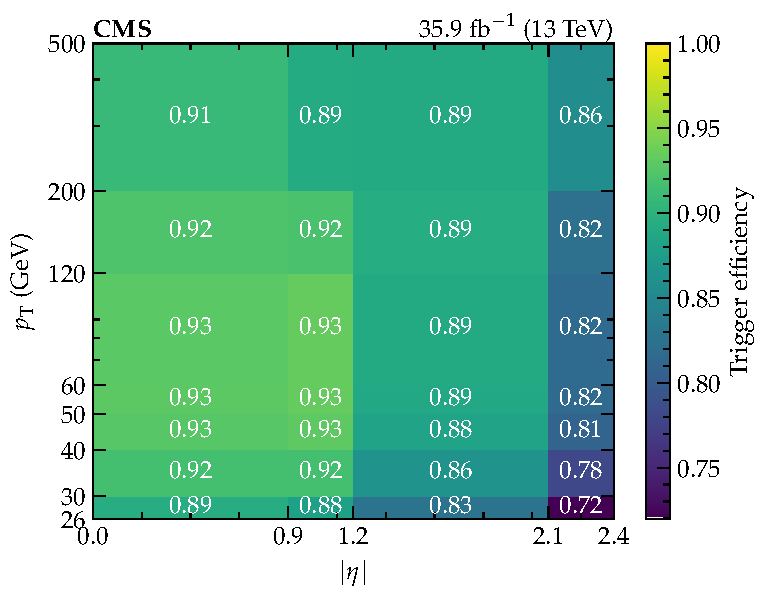
\includegraphics{chapters/041_corrections/images/efficiencies/triggers/muons/muon_RunBCDEF_trigger_efficiency.pdf}
        \caption{Initial data-taking period}
        \label{subfiga:muon-trigger-efficiency}
    \end{subfigure}
    \hfill
    \begin{subfigure}[b]{0.49\textwidth}
        \centering
        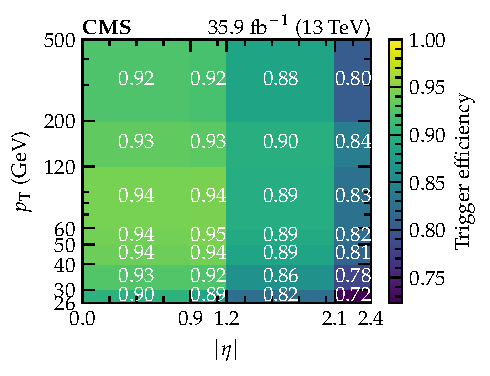
\includegraphics{chapters/041_corrections/images/efficiencies/triggers/muons/muon_RunGH_trigger_efficiency.pdf}
        \caption{Final data-taking period}
        \label{subfigb:muon-trigger-efficiency}
    \end{subfigure}
    \caption[Muon trigger efficiency measurements.]{
        Muon trigger efficiencies parameterised by its \pt and \aeta, split by the data-taking period. To maintain a consistent background rejection, the trigger efficiency is lower in the endcaps where the muon background rate is larger and for low \pt muons where the track reconstruction is poorer. Inefficiencies for high \pt muons result from misidentified charged hadrons or issues in reconstructing the \pt for straight tracks. Most of the trigger efficiency arises from the \HWT decision which is heavily constrained by the timing budget. The differences between the data-taking periods are at most $2\%$, with significant overlap within the uncertainties.
    }
    \label{fig:muon-trigger-efficiency}
\end{figure}

This efficiency, $\varepsilon_i$, is associated to a single muon; however, events collected with higher muon multiplicities were triggered by any of the muons, hence the efficiency associated with the event, $\varepsilon$, for any number of muons is
%
\begin{equation}\label{eq:electron-event-trigger-efficiency}
    \varepsilon = 1 - \prod_{i\in\mathrm{muons}} ( 1 - \varepsilon_i )\ ,
\end{equation}
%
as follows from a binomial distribution where at least one muon must pass the trigger selection. This efficiency scales the MC event weight in regions collected by the muon triggers with a luminosity-weighted average of the initial and final data-taking periods.


\subsection{Electron trigger efficiency}\label{sec:electron-trigger-efficiency}

The electron trigger efficiency measurement \cite{CMS-DP-2017-004} follows a similar procedure to the muons. The analysis selection is applied to the tag and the probe, with relaxed kinematic criteria. The pair of electrons are formed into a \PZ boson candidate with a fit to the invariant mass distribution to extract the signal contribution and determine the efficiency of the electron trigger selection. Systematic uncertainties are determined with the same method detailed for the muon trigger efficiencies. The efficiencies for the electron trigger selection is shown in Fig.~\ref{fig:electron-trigger-efficiency} and follow the same event-based efficiency in Eq.~\ref{eq:electron-event-trigger-efficiency}.

\begin{figure}[htb]
    \centering
    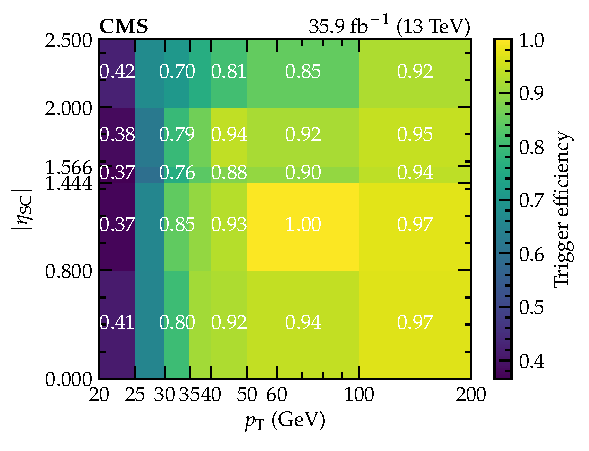
\includegraphics{chapters/041_corrections/images/efficiencies/triggers/electrons/electron_trigger_efficiency.pdf}
    \caption[Electron trigger efficiency.]{
        Electron trigger efficiency with a threshold of ${\pt>\SI{27}{GeV}}$, parameterised with the \pt and absolute supercluster position in $\eta$, $|\eta_{\mathrm{SC}}|$. The low \pt inefficiency is driven by the trigger threshold and the efficiency in the partially uninstrumented gap in the \ECAL is shown in the bin ${1.444<|\eta_{\mathrm{SC}}|<1.566}$.
    }
    \label{fig:electron-trigger-efficiency}
\end{figure}


\subsection{\ptmiss trigger efficiency}\label{sec:met-trigger-efficiency}

The \ptmiss trigger paths collect events for the \metplusjets, \muplusjets, \dimuplusjets, \tauplusjets and the equivalent QCD multijet enriched sidebands. To measure the efficiency in data, an independent set of events are collected using the single muon triggers which may pass or fail the \ptmiss trigger requirements. Furthermore, the \ptmiss triggers primarily place a selection on the recoil which ignores the muons, allowing events to populate the tail of the recoil distribution. No reference trigger is required in MC and the efficiency is extracted from the trigger emulation. The results for \IZvvj, \IWlvj and \IDYllj shown in Fig.~\ref{fig:ptmiss-trigger-eff-noisotrack}, alongside the measurements from data in the \muplusjets and \dimuplusjets regions.

\begin{figure}[htb]
    \centering
    \begin{subfigure}[b]{0.49\textwidth}
        \centering
        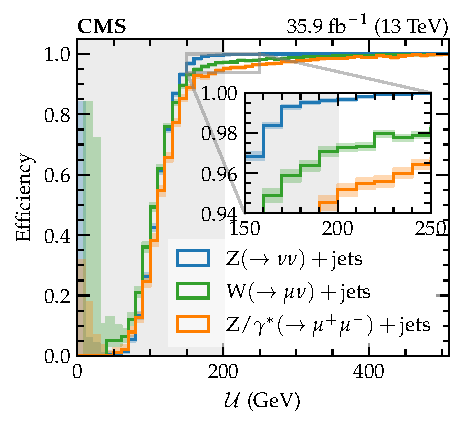
\includegraphics{chapters/041_corrections/images/efficiencies/triggers/met/met_trig_eff_mc_noisotrack.pdf}
        \caption{Simulation}
        \label{subfiga:ptmiss-trigger-eff-noisotrack}
    \end{subfigure}
    \hfill
    \begin{subfigure}[b]{0.49\textwidth}
        \centering
        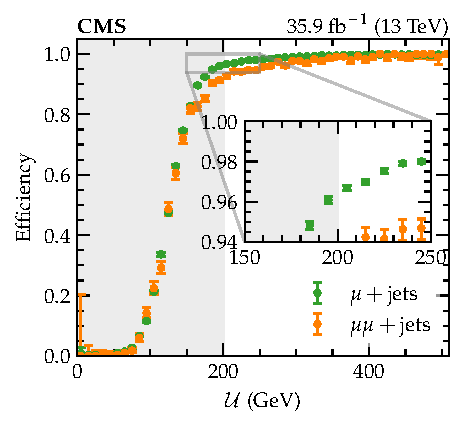
\includegraphics{chapters/041_corrections/images/efficiencies/triggers/met/met_trig_eff_data_noisotrack.pdf}
        \caption{Data}
        \label{subfigb:ptmiss-trigger-eff-noisotrack}
    \end{subfigure}
    \caption[Efficiency of the missing energy triggers in data and simulation.]{
        The dependence of the \ptmiss trigger efficiency on the offline recoil $\mathcal{U}$. The efficiency below $\SI{200}{GeV}$ (grey band) is shown, however, these events are removed in the final analysis. The uncertainty bands represent the $68.2\%$ asymmetric confidence interval on a binomial distribution for a given total number of event with a fraction passing the selection. This band only includes the statistical uncertainty in both simulation and data.
    }
    \label{fig:ptmiss-trigger-eff-noisotrack}
\end{figure}

The lower efficiency measured in data is a result of the evolution of trigger paths to higher thresholds as the beam luminosity increased throughout the 2016 data-taking period, whereas the simulated trigger efficiency is primarily controlled by the lowest threshold. The impact of the evolving trigger paths in data is replicated in MC by applying a scale factor correction determined from the ratio of data to MC efficiency, parameterised with the recoil. However, a clear efficiency difference is observed between the various muon multiplicity regions. In fact, the \SWT muon collection is not perfectly aligned with the offline reconstructed collection causing some muons to be included in the \SWT recoil calculation leading to values below the thresholds. This is significantly mitigated by the addition of a \ptmiss trigger path which selects events with a \ptmiss above $\SI{75}{GeV}$ and an isolated track with ${\pt>\SI{50}{GeV}}$. This recovers events where the muon was misidentified at the \SWT level, however, still classified as an isolated track. The corresponding trigger efficiency measurements are shown in Fig.~\ref{fig:ptmiss-trigger-eff-isotrack}, with a significant improvement between the muon multiplicity regions.
%
\begin{figure}[htb]
    \centering
    \begin{subfigure}[b]{0.49\textwidth}
        \centering
        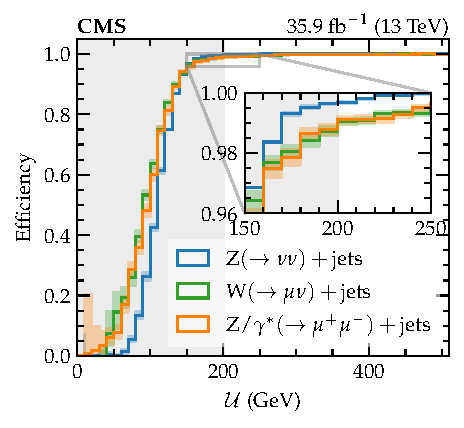
\includegraphics{chapters/041_corrections/images/efficiencies/triggers/met/met_trig_eff_mc.pdf}
        \caption{Simulation}
        \label{subfiga:ptmiss-trigger-eff-isotrack}
    \end{subfigure}
    \hfill
    \begin{subfigure}[b]{0.49\textwidth}
        \centering
        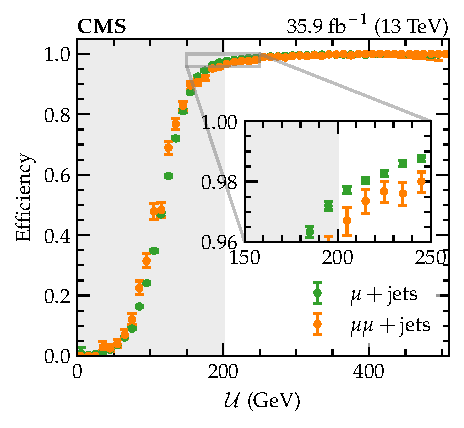
\includegraphics{chapters/041_corrections/images/efficiencies/triggers/met/met_trig_eff_data.pdf}
        \caption{Data}
        \label{subfigb:ptmiss-trigger-eff-isotrack}
    \end{subfigure}
    \caption[Missing energy trigger efficiency measurements with the isolated track selection.]{
        The \ptmiss trigger efficiency measurements similar to Fig.~\ref{fig:ptmiss-trigger-eff-noisotrack}, with the addition of the isolated track selection.
    }
    \label{fig:ptmiss-trigger-eff-isotrack}
\end{figure}

The \ptmiss trigger scale factors are taken from the \muplusjets region where the statistical uncertainty is the lowest. The remaining difference in the scale factors between the \muplusjets and \dimuplusjets regions, shown in {Fig.~\ref{subfiga:ptmiss-trigger-sf}} is taken as a systematic uncertainty to cover residual effects from the muon mismatch between the \SWT and offline. The effect of using the muon triggers as a reference in data is emulated in simulation and the difference between the nominal scale factor is taken as a systematic uncertainty. A final systematic uncertainty is determined by the difference in the scale factors in an independent region, namely the \muplusjets QCD enriched sideband. The scale factors and the associated systematic uncertainties are shown in Fig.~\ref{fig:ptmiss-trigger-sf}.
%
\begin{figure}[htb]
    \centering
    \begin{subfigure}[b]{0.45\textwidth}
        \centering
        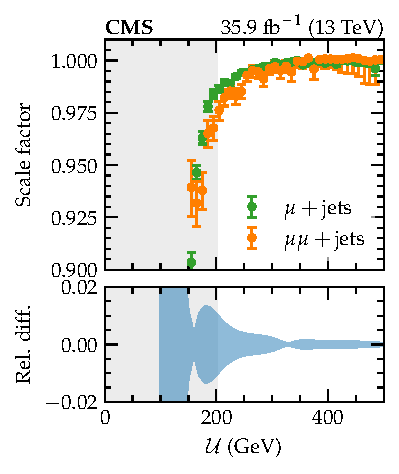
\includegraphics{chapters/041_corrections/images/efficiencies/triggers/met/met_trig_sf_muonsyst.pdf}
        \caption{Muon multiplicity}
        \label{subfiga:ptmiss-trigger-sf}
    \end{subfigure}
    \hfill
    \begin{subfigure}[b]{0.45\textwidth}
        \centering
        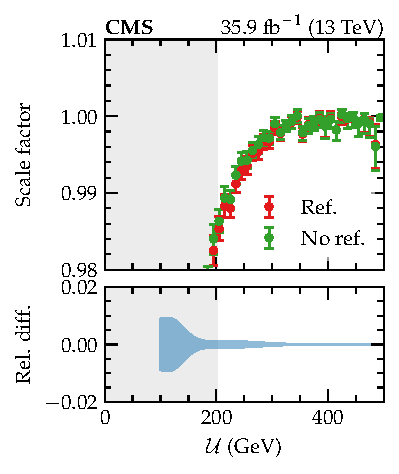
\includegraphics{chapters/041_corrections/images/efficiencies/triggers/met/met_trig_sf_refsyst.pdf}
        \caption{Reference trigger}
        \label{subfigb:ptmiss-trigger-sf}
    \end{subfigure}
    \\
    \begin{subfigure}[b]{0.45\textwidth}
        \centering
        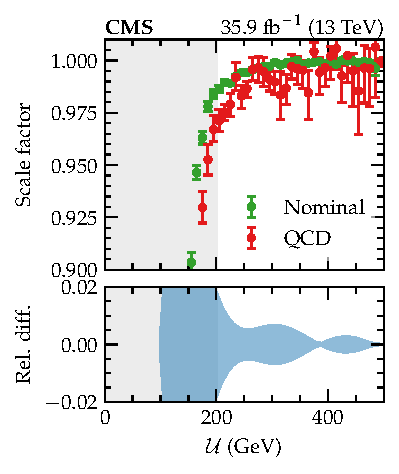
\includegraphics{chapters/041_corrections/images/efficiencies/triggers/met/met_trig_sf_qcdsyst.pdf}
        \caption{Independent sample}
        \label{subfigc:ptmiss-trigger-sf}
    \end{subfigure}
    \caption[Systematic uncertainties associated with the missing energy trigger efficiency measurements.]{
        The \ptmiss trigger scale factors measured for various regions to determine the central correction and relative difference between them for systematic uncertainties. The statistical uncertainties in the scale factors would artificially inflate the scale factors due to correlations between the bins, therefore, it is not used any further in the analysis.
    }
    \label{fig:ptmiss-trigger-sf}
\end{figure}
%
The reference trigger introduces a small bias of less than $0.5\%$, whereas the muon multiplicity systematic covers a $1\%$ effect and the QCD sideband a $2\%$ effect at ${\mathcal{U}=\SI{200}{GeV}}$ and drops off to a negligible level above $\SI{500}{GeV}$ where the efficiencies and scale factors plateau at $1$. The scale factors associated with the \muplusjets region in Fig.~\ref{subfiga:ptmiss-trigger-sf} is applied to all events collected by \ptmiss triggers to primarily correct for the changing conditions during data taking by up to $2\%$, with three systematic uncertainties propagated as alternative templates for the final statistical analysis to cover biases in the scale factor measurement.

The muon multiplicity systematic is decorrelated between the \metplusjets, \muplusjets and \dimuplusjets, allowing the systematic effect to pull each in separate directions. The reference trigger systematic is correlated among all regions. Similarly to the muon multiplicity, the independent sample systematic is decorrelated among all regions. This correlation scheme is a conservative estimate of the underlying uncertainty with the estimation of the \ptmiss trigger scale factors.

\section{Object-based corrections}

Corrections based on the physics objects of an event may alter the weight of the event and will be discussed here, along with corrections to particle kinematics. Furthermore, the selection discussed in Sec.~\ref{sec:categorisation} are not strict requirements on MC events. In particular, events with an object and an associated scale-factor $f$ will contribute to the object selection regions by a weight $f$. However, this event will also contribute to object veto regions by a weight $1-f$ such that the total contribution of the event across all regions becomes $1$, leaving the overall cross-section unchanged. When $f=1$ the strict veto requirements are recovered and the event does not enter the object vetoing regions. The uncertainty on the efficiency of a selection is encoded in the scale-factor, $\delta f$, such that the weight where the event is vetoed is
%
\begin{equation}
    1 - f = 1 - \mathcal{N}_f(f_0,\delta f_1) = 1 - (f_0 + \mathcal{N}_f(0,1)\delta f_1)\ ,
\end{equation}
%
where $f_0$ is the central value of the scale-factor, $\delta f_1$ is its $1\sigma$ variation and $\mathcal{N}_f(\mu,\sigma)$ is a gaussian distributed random variable with a mean $\mu$ and width $\sigma$. Therefore, MC events vetoed may still contribute to a region, albeit weighted down or possibly negatively. Such a procedure is performed with muons, electrons, photons, \Ptauh-leptons and $b$-tagged jets for both the veto and selection definitions.


\subsection{Muons}

Muons are formed from tracks with identification and isolation requirements to reduce misidentification. The efficiency in selecting muons is factorised into
%
\begin{equation}
    \varepsilon_{\mu} = \varepsilon_{\mu}(\mathrm{ID}|\mathrm{track}) \varepsilon_{\mu}(\mathrm{Iso}|\mathrm{ID})\ ,
\end{equation}
%
where the track collection efficiency is near $100\%$ and hence omitted. The parameter $\varepsilon(\mathrm{ID}|\mathrm{track})$ is the identification efficiency for a given set of tracks and $\varepsilon(\mathrm{Iso}|\mathrm{ID})$ is the isolation efficiency given a collection of muons passing identification requirements. Since the analysis uses two muon identification and isolation requirements the efficiency must be measured for both the veto and selection criteria. The measurement is performed using the tag and probe technique with the tag passing a tight set of requirements to ensure minimal misidentifications and the probe defined as a set of tracks or muons with an isolation requirement \cite{CMS-DP-2017-007}. Similarly to the muon trigger efficiency measurements, the events are split into bins of lepton \pt and $\eta$. A likelihood fit to the invariant mass distribution of each bin is independently performed to extract the signal contribution for the numerator and denominator of the efficiency: probes passing the isolation and identification requirements and all probes, respectively. A similar approach is performed in MC. % WRONG:, however, the distinction of signal events is known, bypassing the need for a fit allowing for the simple counting of events.

During the 2016 data-taking period, saturation issues in the pre-amplifier chips for the tracker resulted in a loss of hits. This effect was mitigated in the later part of this period and further reduced by a re-processing of the data. Nevertheless, the identification and isolation efficiencies are split into the initial part and final part of the data-taking period. The ratio of the efficiencies measured in data and MC for each period is shown in Fig.~\ref{fig:muon-id-scale-factors} and \ref{fig:muon-iso-scale-factors} and subsequently the product of the identification and isolation scale-factors is applied as a correction to MC.

\begin{figure}[htb]
    \centering
    \begin{subfigure}[b]{0.49\textwidth}
        \centering
        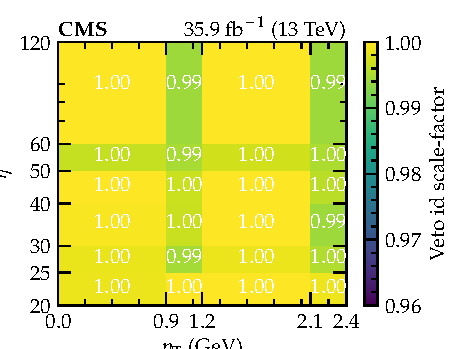
\includegraphics{chapters/041_corrections/images/efficiencies/objects/muons/muon_id_loose_runbf.pdf}
        \caption{Initial data-taking period}
        \label{subfiga:muon-id-scale-factors}
    \end{subfigure}
    \hfill
    \begin{subfigure}[b]{0.49\textwidth}
        \centering
        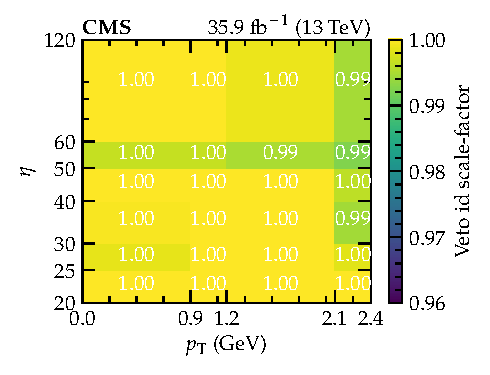
\includegraphics{chapters/041_corrections/images/efficiencies/objects/muons/muon_id_loose_rungh.pdf}
        \caption{Final data-taking period}
        \label{subfigb:muon-id-scale-factors}
    \end{subfigure}
    \\
    \begin{subfigure}[b]{0.49\textwidth}
        \centering
        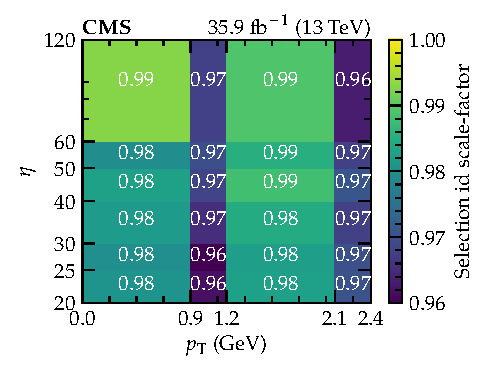
\includegraphics{chapters/041_corrections/images/efficiencies/objects/muons/muon_id_tight_runbf.pdf}
        \caption{Initial data-taking period}
        \label{subfigc:muon-id-scale-factors}
    \end{subfigure}
    \hfill
    \begin{subfigure}[b]{0.49\textwidth}
        \centering
        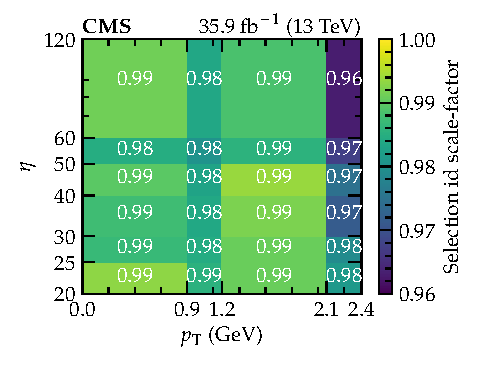
\includegraphics{chapters/041_corrections/images/efficiencies/objects/muons/muon_id_tight_rungh.pdf}
        \caption{Final data-taking period}
        \label{subfigd:muon-id-scale-factors}
    \end{subfigure}
    \caption[Corrections to simulated muon identification efficiencies.]{
        Muon identification (id) scale corrections applied to MC, parameterised with the muon \pt and \aeta. The top row shows the scale-factors for veto muons with corrections less than $1\%$ as a result of the basic selection. The bottom row shows the scale-factors for selection muons with corrections from {$1$--$4\%$} with the largest discrepancies on the edges of the endcaps (${0.9<\aeta<1.2}$ and ${2.1<\aeta<2.4}$) where the muon identification modelling does not perform as well in MC. 
    }
    \label{fig:muon-id-scale-factors}
\end{figure}

\begin{figure}[htb]
    \centering
    \begin{subfigure}[b]{0.49\textwidth}
        \centering
        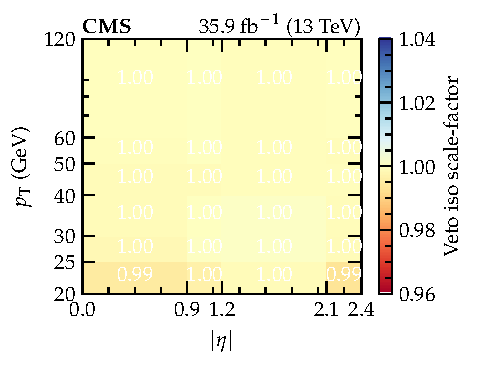
\includegraphics{chapters/041_corrections/images/efficiencies/objects/muons/muon_iso_loose_runbf.pdf}
        \caption{Initial data-taking period}
        \label{subfiga:muon-iso-scale-factors}
    \end{subfigure}
    \hfill
    \begin{subfigure}[b]{0.49\textwidth}
        \centering
        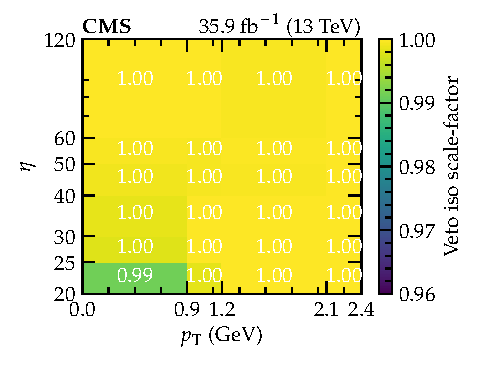
\includegraphics{chapters/041_corrections/images/efficiencies/objects/muons/muon_iso_loose_rungh.pdf}
        \caption{Final data-taking period}
        \label{subfigb:muon-iso-scale-factors}
    \end{subfigure}
    \\
    \begin{subfigure}[b]{0.49\textwidth}
        \centering
        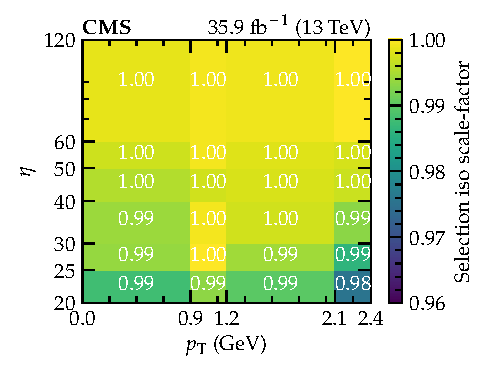
\includegraphics{chapters/041_corrections/images/efficiencies/objects/muons/muon_iso_tight_runbf.pdf}
        \caption{Initial data-taking period}
        \label{subfigc:muon-iso-scale-factors}
    \end{subfigure}
    \hfill
    \begin{subfigure}[b]{0.49\textwidth}
        \centering
        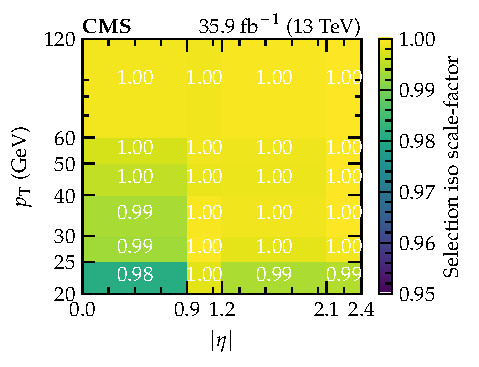
\includegraphics{chapters/041_corrections/images/efficiencies/objects/muons/muon_iso_tight_rungh.pdf}
        \caption{Final data-taking period}
        \label{subfigd:muon-iso-scale-factors}
    \end{subfigure}
    \caption[Corrections to simulated muon isolation efficiencies.]{
        Muon isolation (iso) scale corrections applied to MC, parameterised with the muon \pt and \aeta. The modelling of the isolation in MC is better than the identification with at most $2\%$ difference for selection muons with discrepancies only in the low \pt region. The $z$-axis range is the same as the muon identification scale factor in Fig.~\ref{fig:muon-id-scale-factors}.
    }
    \label{fig:muon-iso-scale-factors}
\end{figure}


\subsection{Electrons and Photons}

The efficiency of the identification and isolation of electromagnetic showers are measured with the tag and probe technique in a similar manner to the muon-based efficiencies \cite{CMS-DP-2017-004}. A fit to the invariant mass distribution of electron pairs is performed to extract the signal yield in various probe \pt and $\eta$ bins. This allows the efficiencies to be determined with analogous measurements in MC with the counting method. Systematic uncertainties are determined from the variation in efficiencies from altering the tag selection, signal model (template from MC or fully parametric), background model, MC generator (LO against NLO), and additional sources for the photon identification efficiency to account for differences in the electron and photon showers. The ratio of the efficiency in data and MC is determined, shown in Fig.~\ref{fig:egamma-id-iso-efficiency} and applied as a correction to MC.

\begin{figure}[htb]
    \centering
    \begin{subfigure}[b]{0.49\textwidth}
        \centering
        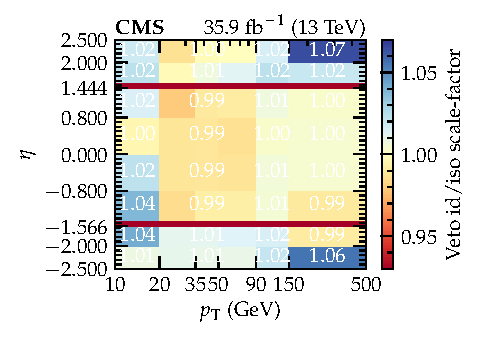
\includegraphics{chapters/041_corrections/images/efficiencies/objects/electrons/electron_idiso_veto_sf.pdf}
        \caption{Electron veto}
        \label{subfiga:egamma-id-iso-efficiency}
    \end{subfigure}
    \hfill
    \begin{subfigure}[b]{0.49\textwidth}
        \centering
        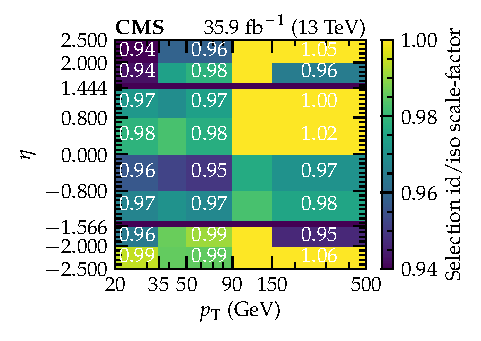
\includegraphics{chapters/041_corrections/images/efficiencies/objects/electrons/electron_idiso_tight_sf.pdf}
        \caption{Electron selection}
        \label{subfigb:egamma-id-iso-efficiency}
    \end{subfigure}
    \\
    \begin{subfigure}[b]{0.49\textwidth}
        \centering
        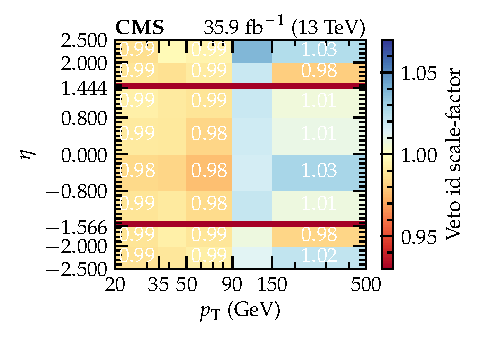
\includegraphics{chapters/041_corrections/images/efficiencies/objects/photons/photon_id_veto_sf.pdf}
        \caption{Photon veto}
        \label{subfigc:egamma-id-iso-efficiency}
    \end{subfigure}
%    \hfill
%    \begin{subfigure}[b]{0.49\textwidth}
%        \centering
%        \includegraphics{}
%        \caption{Caption}
%        \label{subfigd:egamma-id-iso-efficiency}
%    \end{subfigure}
    \caption[Corrections to simulated electron and photon identification efficiencies.]{
        Electron and photon identification scale-factors for the various analysis-level object categorisations. The bands at ${1.444<\aeta<1.566}$ correspond to the partially uninstrumented gap in the \ECAL. The corrections typically arise from the mismodelling of the interactions of electromagnetic particles with the inner detector material resulting in photon conversions and Bremsstrahlung, particularly in the endcaps. 
    }
    \label{fig:egamma-id-iso-efficiency}
\end{figure}

In addition, the efficiency for the reconstruction of GSF tracks matched to \ECAL deposits is measured with the same method and shown in Fig.~\ref{fig:electron-reco-efficiency}. Similarly, the efficiency from vetoing photons with consistent track in the pixel detector is measured with a similar method in \IDYmmg, where the tag consists of a muon pair and the probe a final state radiated photon. The ratio of the efficiency in data and MC for the GSF track veto is shown in Fig.~\ref{fig:photon-trackveto-efficiency}.

\begin{figure}[htb]
    \centering
    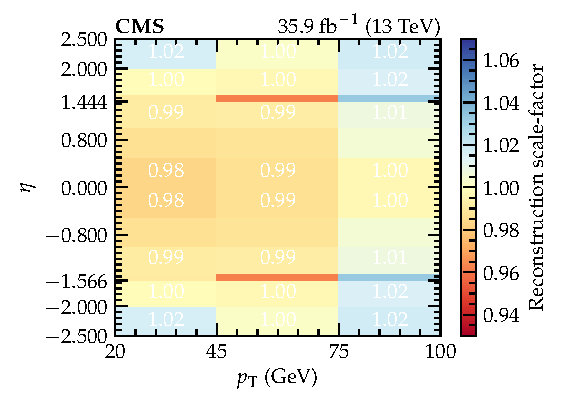
\includegraphics{chapters/041_corrections/images/efficiencies/objects/electrons/electron_reco_sf.pdf}
    \caption[Corrections to simulated electron reconstruction efficiency.]{
        Electron scale-factors associated with the reconstruction of electrons from tracks and \ECAL deposits. The \ECAL partially uninstrumented gap at ${1.444<\aeta<1.566}$. Mostly a good agreement between data and MC with deviations for low \pt and endcap electrons, again affected by material interactions.
    }
    \label{fig:electron-reco-efficiency}
\end{figure}

\begin{figure}[htb]
    \centering
    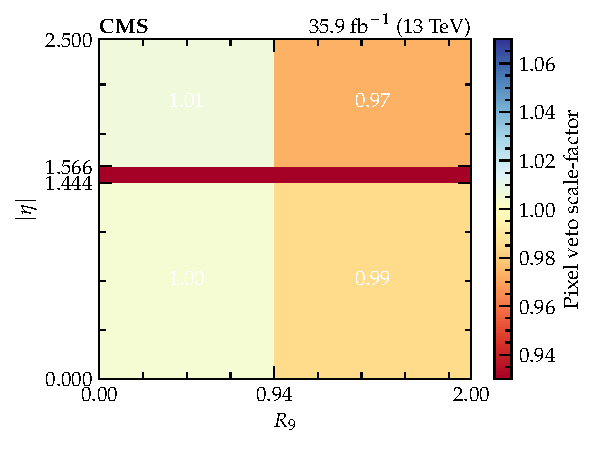
\includegraphics{chapters/041_corrections/images/efficiencies/objects/photons/photon_pixelveto_sf.pdf}
    \caption[Corrections to photon pixel veto efficiency.]{
        Photon pixel veto scale-factors parameterised by \aeta and $R_9$, the ratio of energy deposited in a $3\times 3$ grid of crystals surrounding the seeding crystal with the full supercrystal energy. The $R_9$ variable is sensitive to unconverted ($R_9\lesssim 0.94$) and converted ($R_9\gtrsim 0.94$) photons. The pixel veto removes photon candidates matched to tracks in the pixel detector.
    }
    \label{fig:photon-trackveto-efficiency}
\end{figure}

Finally, the difference in the scale and resolution of electrons and photons in data and MC is measured from the impact on the mean and width of the invariant mass distribution in \IDYee events. A fit to the \PZ lineshape is performed to extract the mean and width in data and MC. The observed difference is used as a correction to electron and photon energies with associated systematic uncertainties from the signal and background models, MC generator and differences between the electron and photon showers.

% TODO: give a reference or attach the associated result?


\subsection{Jets}

The detector response to objects, especially the cluster of particles in jets, is not linear. Therefore, a set of jet energy corrections are measured and applied to map the reconstructed jet energy to the particle-level equivalent (the energy of all generated particles originating from the parton excluding neutrinos). A factorised approach is implemented with each level accounting for different effects \cite{Khachatryan:2016kdb}.

The first step mitigates the contribution of particles from pileup vertices which fall within the cone of the jet. This contribution is determined with the random cone method in zero bias events and in simulations without any hard interactions. Zero bias events are collected by randomly selecting collisions regardless of their content. Since the hard interaction cross-section is small this typically selected events with pileup interactions. The random cone method consists of placing a random set of jet cones in a zero bias event, clustering the particles falling within these cones, and determining the energies of these jets. This energy represents the contribution to a jet from pileup and is parameterised by the event energy density and jet \pt and $\eta$. A systematic uncertainty is determined by comparing the correction from the random cone method to the generator-level in MC.

The second step involves the correction to particle-level jets. Again, this is determined from QCD dijet simulations by comparing the reconstructed jet \pt to particle-level \pt, parameterised by the jet \pt and $\eta$. A systematic uncertainty is determined for this correction as a result of its dependence on the underlying detector calibrations with results from test beam studies.

The third and final step attempts to resolve residual differences between data and MC. These corrections are applied to data since the aim is to replicate the particle-level description which is only available in simulation. This step is split into two stages: the first is an $\eta$-dependent correction determined from dijet events with barrel jets used as a reference, and a second a \pt-dependent scale difference between data and MC determined from \IDYllj, \Igj and QCD multijet events. In these processes the jet energy response is studied by comparing reconstructed jets to particle-level jets on a jet-by-jet basis and also the whole hadronic activity from the correlation of a particle-level jet to the missing transverse energy of the event. These methods do not fully capture the dependence as a result of the correlation between initial (ISR) or final state radiated (FSR) jets. Therefore, an additional correction is determined by probing the $\eta$-dependent corrections with a selection to enhance the effect of this correlation. Along with these corrections are associated systematic uncertainties to cover the modelling in MC from an alternative event generator, statistical uncertainties in the data due to trigger prescales, dependence of the corrections over the data taking period, constituent particle energy uncertainties, and the residual difference between the dijet, \Igj and \IDYllj samples after all corrections have been applied.

In addition to the jet energy response difference between data and MC the resolution is corrected for by comparing the balance of jets in a dijet event. The scale determined to correct the MC resolution of the dijet balance is applied to MC jets by smearing their energies with a random variable sampled from a gaussian distribution with a scaled width. Systematic uncertainties are determined by comparing the results to the particle-level imbalance, the effect of removing particles below $\SI{10}{GeV}$, non-gaussian tails in the resolution due to rare detector effects and the \pt-dependence is propagated through the smearing.

All these corrections, and uncertainties, are propagated through all jet-related quantities such as the missing transverse momentum where the jet energy correction $k_i$, encoding both scale and resolution corrections, results in a shift in the \ptmiss according to
%
\begin{equation}\label{eq:ptmiss-type1-corr}
    \vecptmiss \mapsto \vecptmiss + \sum_{i\in\mathrm{jets}}\vec{p}_{\mathrm{T},i} \left( 1 - k_i \right)\ ,
\end{equation}
%
where the sum is over clustered jets, i.e. ${\pt>\SI{15}{GeV}}$. The corrected \ptmiss quantity is used in subsequent derivatives such as the recoil.


\subsubsection{\Ptauh-tagged jets}

The jet energy corrections discussed above are determined under the assumption that the jet originates from a parton. Therefore, the corrections are not applied to \Ptauh-tagged jets, instead a scale-factor is determined to correct the efficiency of \Ptauh-lepton identification in MC. The efficiency in data is measured using the tag and probe method in \IDYtt decays, where one $\tau$-lepton decays into a well reconstructed muon to tag the event and the other into one of the hadronic decay modes to probe the identification. A fit is performed to the invariant mass of the visible particles to extract the signal contribution with templates taken from MC for the signal and most backgrounds. Systematic uncertainties on the identification efficiency are determined from the background normalisation, \ptmiss uncertainties and limited sample sizes \cite{Sirunyan:2018pgf}. The scale-factors and uncertainties to correct the \Ptauh identification efficiency in MC is shown in Fig.~\ref{fig:tau-id-scale-factors}.

\begin{figure}[htb]
    \centering
    \begin{subfigure}[b]{0.49\textwidth}
        \centering
        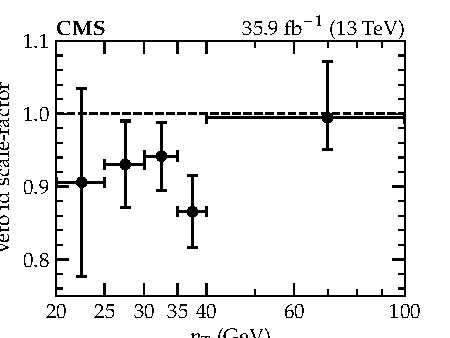
\includegraphics{chapters/041_corrections/images/efficiencies/objects/taus/tau_id_veto_sf.pdf}
        \caption{Veto identification}
        \label{subfiga:tau-id-scale-factors}
    \end{subfigure}
    \begin{subfigure}[b]{0.49\textwidth}
        \centering
        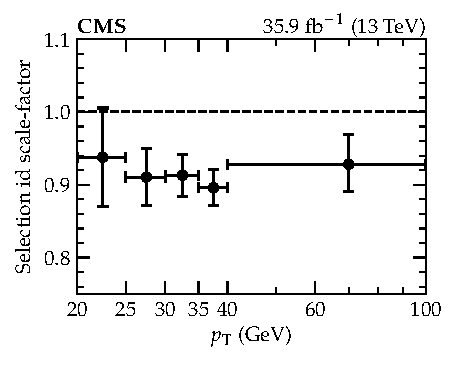
\includegraphics{chapters/041_corrections/images/efficiencies/objects/taus/tau_id_tight_sf.pdf}
        \caption{Selection identification}
        \label{subfigb:tau-id-scale-factors}
    \end{subfigure}
    \caption[Corrections to $\tau$-tagged jet efficiency.]{
        \Ptauh identification scale-factors parameterised by the \Ptauh \pt. The dashed line is placed at a scale-factor of $1$. The veto category is mostly consistent with $1$ while the selection category deviates by {$5$--$10\%$} as a result of attempting to reduce misidentifications by probing the complex structure of multiple hadronic $\tau$-lepton decays.
    }
    \label{fig:tau-id-scale-factors}
\end{figure}


\subsubsection{$b$-tagged jets}

Jets tagged as originating from $b$-hadrons have the jet energy corrections applied, however, the $b$-tagging discriminant is not perfectly modelled in MC due to detector simulation limitations and the accuracy of the generator modelling the parton shower and hadronisation. Therefore, a scale-factor is determined for the efficiency of $b$-tagging jets from QCD multijet, muon-enriched jet, dilepton \Itt and single lepton \Itt samples \cite{Sirunyan:2017ezt}. The efficiency is parameterised by the jet flavour (grouped in $b$, $c$ and $udsg$ flavours), \pt and $\eta$. In simulation, the tagging efficiency is calculated by matching jets to generated jets with a particular hadron flavour. Meanwhile, the data efficiency is measured with a pure sample with jets of a certain hadron flavour using a selection which does not bias the jets with respect to the variables in the tagging algorithm. Systematic uncertainties associated to the $b$-tag scale-factors are determined by varying background normalisations, branching fractions of hadronic decays within the PDG uncertainties, reweighting the distribution of the number of tracks, jet energy scale uncertainties, electron and muon efficiencies and theoretical uncertainties from the event generators. The scale-factors associated with the $i$-enumerated $b$-tagged jet, $f_i$, is measured with a parameteric form with the \pt of the jet given by
%
\begin{equation}
    f_i(\pt) =
    \begin{cases}
        p_0 \left(1 + p_1 \pt\right)/\left(1 + p_2 \pt\right), & \text{$c$ and $b$-hadrons}\\
        p_0 + p_1 \pt + p_2 \pt^2 + p_3 \pt^3, & \text{$udsg$-hadrons}
    \end{cases}
\end{equation}
%
where $p_0$, $p_1$, $p_2$ and $p_3$ are parameters measured from a fit to the scale-factors in categories based on the jet flavour, \pt and $\eta$. In the context of this analysis, $b$-tagged jets are vetoed, therefore the event weight becomes
%
\begin{equation}
    w \mapsto w \prod_{i\in\mathrm{b-jets}} (1 - f_i)\ .
\end{equation}


\section{Luminosity}

The integrated luminosity $\mathcal{L}$ measured for the data-taking period directly scales the weight of a MC event. At \CMS the pixels, drift tubes, HF and other detectors perform complimentary measurements of the luminosity by rate counting, $R$, for visible processes with a cross-section $\sigma_{\mathrm{vis}}$. The luminosity is determined as
%
\begin{equation}
    \mathcal{L} = \frac{R}{\sigma_{\mathrm{vis}}}\ ,
\end{equation}
%
where the visible cross-section and calibrations of each detector is performed by conducting Van der Meer scans \cite{vanderMeer:296752} prior to data-taking collisions. The data collected during 2016 corresponds to an integrated luminosity of ${\SI{35.9}{fb^{-1}}}$ with uncertainties from the precision of the visible cross-section and calibration measurements along with extrapolations to data-taking collisions resulting in a $2.5\%$ uncertainty \cite{CMS:2017sdi} on the luminosity measurement. 

\section{Pileup reweighting}

The pileup overlay applied to each simulated event is generated by the \PYTHIA package with the number of pileup vertices sampled from a poisson distribution with a tail to higher vertex multiplicities, as shown in Fig.~\ref{fig:pu-reweighting}. In data, for a given instantaneous luminosity, the number of pileup vertices is expected to be poisson distributed. Therefore, a reweighting procedure corrects the MC distribution to reflect that observed in data, without altering the normalisation determined from the product of the process cross-section and the integrated luminosity. The number of interactions in data is estimated from the measured luminosity in each bunch crossing and the average total inelastic cross-section. Furthermore, data measurements are averaged over periods of constant instantaneous luminosity to compare with the mean of poisson distribution sampled in MC, rather than the number of vertices in a particular event. The total inelastic cross-section, measured by \CMS, is ${\SI{69.2}{mb}}$, with an uncertainty of $4.6\%$ represented by the bands in Fig.~\ref{fig:pu-reweighting}. These $\pm 1\sigma$ variations are propagated through to the \PZ invisible width measurement.

\begin{figure}[htb]
    \centering
    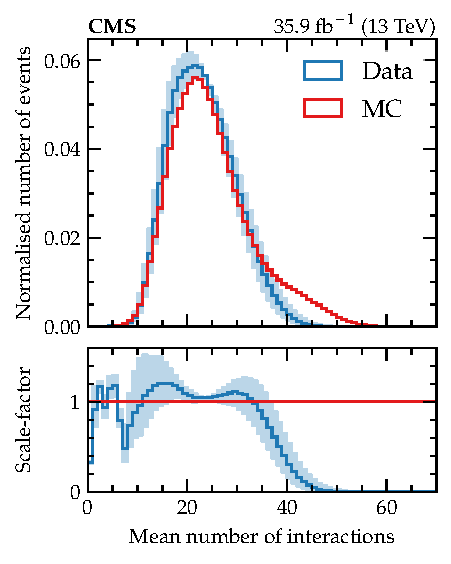
\includegraphics{chapters/041_corrections/images/pileup/pileup.pdf}
    \caption[Pileup distribution in data and simulation for reweighting.]{
         The distribution of the mean number of interactions the events are sampled from, closely following a poisson distribution with a long tail in MC. The uncertainty band is determined by varying the total inelastic cross-section by $4.6\%$. The average of the mean number of interactions in data is $22.7$, under the \LHC beam conditions provided during 2016.
    }
    \label{fig:pu-reweighting}
\end{figure}


\section{\ECAL timing degradation}

A gradual degradation in the \ECAL timing has caused some \HWT \ECAL towers to be associated with the incorrect bunch crossing (BX). The \HWT logic prevents three successive bunch crossings to be accepted to avoid buffer overflows. Therefore, the deposit in the \ECAL is wrongly associated to an early crossing which may lead to a \HWT accept, later discarded in the \SWT where the timing issue is not present. However, the correct crossing is vetoed by the \HWT logic resulting in a loss in efficiency in the data collection. This primarily affects events with \ECAL deposits in the endcaps where the timing degradation is most prevalent.

The efficiency of this issue is measured by collecting immune events which occur three bunch crossings after a \HWT accepted crossing. The immune event is labelled as $\mathrm{BX}+0$ and the $n$-enumerated crossing before as $\mathrm{BX}-n$ and after as $\mathrm{BX}+n$. Since $\mathrm{BX}-3$ is accepted by the \HWT the crossings $\mathrm{BX}-2$ and $\mathrm{BX}-1$ are vetoed, hence they cannot veto $\mathrm{BX}+0$. Although these events are immune to the issue, they are tagged as events that would have been vetoed if $\mathrm{BX}-1$ or $\mathrm{BX}-2$ contains a \HWT object from $\mathrm{BX}+0$. However, the event is recovered since it is protected by the preceding $\mathrm{BX}-3$. The efficiency is determined from the set of immune events, with and without a problematic \HWT object. It is parameterised by the \pt and $\eta$ of the reconstructed jet associated with the problematic \HWT object. In MC the efficiency of this issue is determined from a product over the measured efficiencies associated to each object which is applied as a correction to the event weight.


\section{Theory corrections}\label{sec:theory-corrections}

The cross-section applied directly to the event weight of a MC process is calculated by theoretical predictions of the highest available order in the strong and electroweak (EW) coupling constants. Associated systematic uncertainties are determined by varying the QCD factorisation and renormalisation scale up and down by a factor of two. This is done for the independent variation of the two scales and the fully correlated variation, with the largest of the six variations taken as the systematic uncertainty. In addition, the uncertainties from the measurements of the sampled \NNPDF parton distribution functions (PDF) \cite{Ball:2014uwa} are propagated by 100 variations, each randomly sampled from the original distributions of the PDFs.

An alternative method is applied to the signal and dominant \IVj processes.  These are generated at NLO in the strong coupling constant, however, instead of scaling the normalisation up to the highest order available, a reweighting of the boson \pt distribution is performed for a more accurate prediction.  This approach reweights the MC to NNLO QCD and NLO EW with next-to-leading logarithm (NLL) EW corrections \cite{Lindert:2017olm}. This procedure scales the cross-section parameterised by the boson \pt, determined from the generated decay products (with photons within ${\Delta R<0.1}$ of a charged lepton summed into their 4-momentum). Systematic uncertainties determined for the QCD corrections include variations in the factorisation and renormalisation scales with the addition of a possible boson \pt dependence and encoding the correlation between the \IZj and \IWj processes.

Another set of systematic uncertainties are determined for the EW corrections to cover higher-order effects and an additional systematic uncertainty on unaccounted contributions from diagrams of mixed order in the strong and EW coupling constants by taking the difference between an additive and factorised combination of the separate QCD and EW corrections. The PDF uncertainties are propagated with the same procedure as for other generated processes. The full set of uncertainties are detailed in Tab.~\ref{tab:qcdew-systematics}, with the correlation scheme \cite{Lindert:2017olm}.

\begin{table}[htb]
    \centering
    \begin{tabular}{lccccp{6cm}}
        \hline \hline
        Label & \IWj & \IZj & Correlation & Other & Description \\
        \hline
        \uncqcdone & \checkmark & \checkmark & \checkmark & \checkmark & Factorisation and renormalisation scale variations. \\
        \uncqcdtwo & \checkmark & \checkmark & \checkmark & & Boson \pt dependence of the QCD scales. \\
        \uncqcdthr & \checkmark & & & & Correlations between QCD effects in \IZj and \IWj processes, relative to \IZj. \\
        \hline
        \uncewone & \checkmark & \checkmark & \checkmark & & Universal unknown Sudakov logarithms beyond NNLO. \\
        \uncewtwo & \checkmark & \checkmark & & & $5\%$ of the absolute full NLO EW correction for a conservative estimate of non-Sudakov factors. \\
        \uncewthr & \checkmark & \checkmark & & & Difference between a naive and rigorous NLL Sudakov approximation. \\
        \hline
        \uncqcdewmix & \checkmark & \checkmark & \checkmark & & Mixing terms with strong and EW coupling vertices. \\
        \hline
        \uncpdf & \checkmark & \checkmark & \checkmark & \checkmark & 100 PDF variations. \\
        \hline \hline
    \end{tabular}
    \caption[Summary of the uncertainties associated to theoretical predictions.]{
        All systematic uncertainties included from the theory prediction of process cross-sections with a tick for which processes the uncertainty affects split into either \IWj, \IZj or other processes. A tick in the correlation column signifies the full correlation between the \IWj and \IZj processes, otherwise the uncertainty is uncorrelated. A brief description of each uncertainty is given.
    }
    \label{tab:qcdew-systematics}
\end{table}


\section{\ptmiss calibration}\label{sec:ptmiss-calib}

The missing energy appears in the analysis selection as the recoil variable $\mathcal{U}$, with the criteria ${\recoil>\SI{200}{GeV}}$ driven by the trigger thresholds. This parameter acts as a proxy for the boson \pt in \IVj processes. The simulation modelling of the recoil as a proxy for the boson \pt is confirmed in data by calibration with \diellplusjets events. These events have an independent measure of the boson \pt through the dilepton \pt. Discrepancies in the modelling are typically due to the nonlinear response of the calorimeters to hadronic particles and the modelling of interactions with the inner detector. A schematic diagram of the event kinematics is shown in Fig.~\ref{fig:recoil-calib-diagram}.

\begin{figure}[htb]
    \centering
    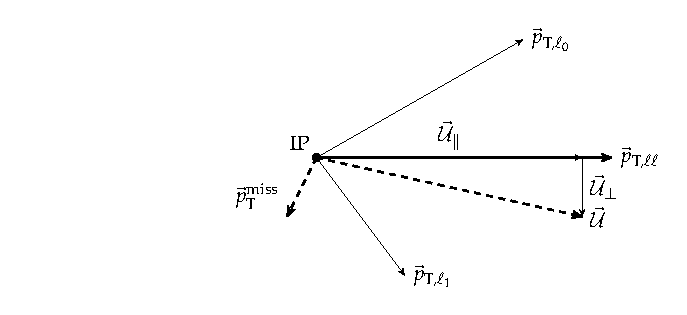
\includegraphics{diagrams/tikz/recoil_calib/recoil_calib.pdf}
    \caption[Kinematics diagram of a \IDYllj events.]{
        The $x$-$y$ plane kinematics of a \IDYllj event showing the momenta of the leading lepton $\ell_0$, subleading lepton $\ell_1$, their sum \vecptll; the missing transverse momentum \vecptmiss; the recoil, defined as $\vecrecoil=\vecptll+\vecptmiss$; and the parallel and perpendicular components of the recoil along the \vecptll axis, \vecrecoilpara and \vecrecoilperp respectively. The interaction point (IP) is at the centre. The missing energy is spurious as a result of mismeasurement, particles out of acceptance or from pileup vertices, and noise.
    }
    \label{fig:recoil-calib-diagram}
\end{figure}

The parallel component \vecrecoilpara probes imperfect calibrations of the \ptmiss typically from mismeasurement in the hadronic system, whereas the perpendicular component \vecrecoilperp probes the isotropic nature of the energy fluctuations from noise and pileup particles. The magnitude of the \vecrecoilpara subtracted by \vecptll along with the magnitude of the \vecrecoilperp are expected to be centred on the scale of the \ptmiss and a width corresponding to its resolution. The distribution of these variables is shown in Fig.~\ref{fig:recoil-calib-dists}.

\begin{figure}[htb]
    \centering
    \begin{subfigure}[b]{0.49\textwidth}
        \centering
        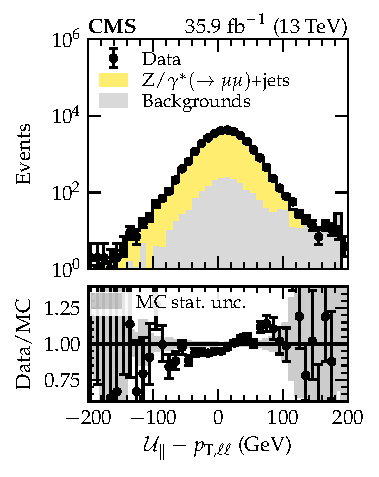
\includegraphics{chapters/041_corrections/images/ptmiss_calib/metres_para_mm_incdist.pdf}
        \caption{Dimuon parallel component}
        \label{subfiga:recoil-calib-dists}
    \end{subfigure}
    \hfill
    \begin{subfigure}[b]{0.49\textwidth}
        \centering
        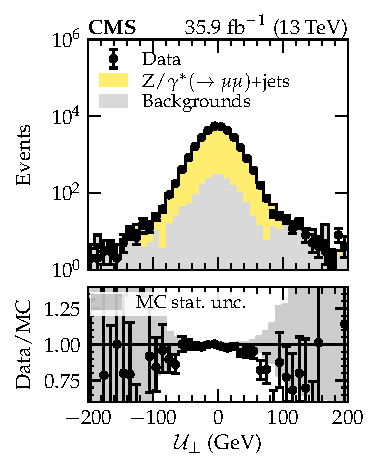
\includegraphics{chapters/041_corrections/images/ptmiss_calib/metres_perp_mm_incdist.pdf}
        \caption{Dimuon perpendicular component}
        \label{subfigb:recoil-calib-dists}
    \end{subfigure}
    \\
    \begin{subfigure}[b]{0.49\textwidth}
        \centering
        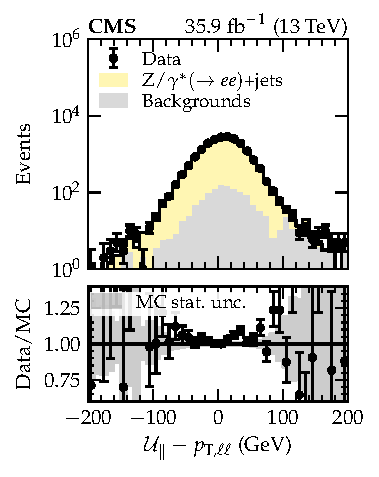
\includegraphics{chapters/041_corrections/images/ptmiss_calib/metres_para_ee_incdist.pdf}
        \caption{Dielectron parallel component}
        \label{subfigc:recoil-calib-dists}
    \end{subfigure}
    \hfill
    \begin{subfigure}[b]{0.49\textwidth}
        \centering
        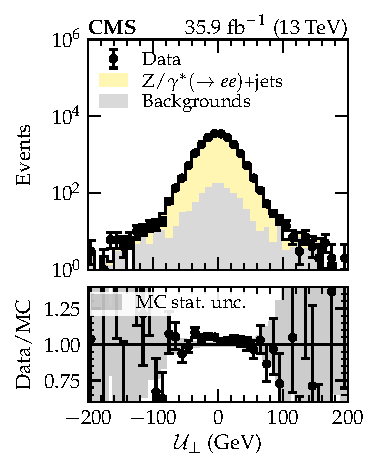
\includegraphics{chapters/041_corrections/images/ptmiss_calib/metres_perp_ee_incdist.pdf}
        \caption{Dielectron perpendicular component}
        \label{subfigd:recoil-calib-dists}
    \end{subfigure}
    \caption[Recoil distributions in dilepton final states.]{
        Distributions of the $\mathcal{U}_{\parallel}-\ptll$ and $\mathcal{U}_{\perp}$ for the \dimuplusjets and \dieleplusjets regions with the $\mathcal{U}$ requirement relaxed to ${\mathcal{U}>\SI{100}{GeV}}$ to probe their dependence with lower recoil while maintaining a reliable \ptmiss trigger scale factor measurement.
    }
    \label{fig:recoil-calib-dists}
\end{figure}

A maximum likelihood fit is performed to the data, with backgrounds subtracted by a template determined from MC, and the signal modelled as a Voigtian --- the convolution of a Gaussian with a Breit-Wigner which captures the peaking nature of the distribution smeared by the detector resolution. A large tail is seen in the backgrounds within the \recoilpara distribution as a result of processes with invisible particles leading to real \ptmiss, whereas the background in the \recoilperp distribution is symmetric. The Voigtian fit is also performed on the signal MC distribution to estimate the scale and resolution in MC. The scale is given by the mean of the distribution while the width is extracted as
%
\begin{equation}
    \sigma_V = \frac{1}{\sqrt{2\ln 2}}\left(0.5346\gamma + \sqrt{0.2166\gamma^2 + 2\ln(2) \sigma^2}\right)\ ,
\end{equation}
%
for a Voigtian with a Gaussian centred on $u_0$ and a width $\sigma$ and a Breit-Wigner also centred on $u_0$ and a width $\gamma$. When $\gamma\ll\sigma$ the distribution reduces to a Gaussian. These parameters are extracted from a fit in bins of \ptll since the detector resolution varies with the energy of particle tracks and deposits. The distribution of \ptll is shown in Fig.~\ref{fig:metres-zpt} which is divided into 20 bins of equal events in data, rounded to the nearest ${\SI{5}{GeV}}$ for convenience.
%
\begin{figure}[htb]
    \centering
    \begin{subfigure}[b]{0.49\textwidth}
        \centering
        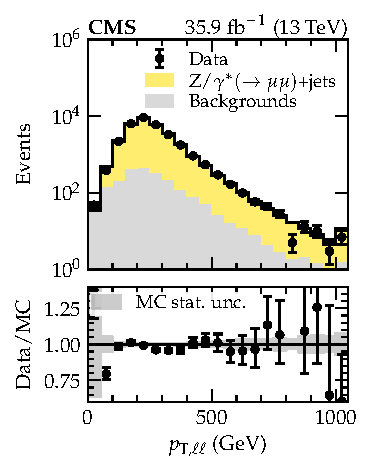
\includegraphics{chapters/041_corrections/images/ptmiss_calib/metres_ptll_mm_incdist.pdf}
        \caption{\dimuplusjets}
        \label{subfiga:metres-zpt}
    \end{subfigure}
    \begin{subfigure}[b]{0.49\textwidth}
        \centering
        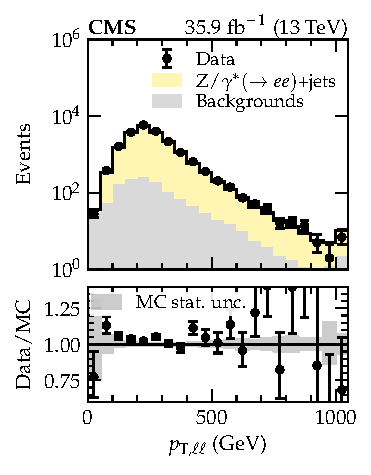
\includegraphics{chapters/041_corrections/images/ptmiss_calib/metres_ptll_ee_incdist.pdf}
        \caption{\dieleplusjets}
        \label{subfigb:metres-zpt}
    \end{subfigure}
    \caption[Dilepton \pt distribution.]{
        Dilepton \ptll distributions peaking near $\SI{200}{GeV}$ as a result of the kinematic selection placed on the recoil and the leading jet.
    }
    \label{fig:metres-zpt}
\end{figure}
%
The fit is performed in each \ptll bin with $\SI{10}{GeV}$ bins in the $\mathcal{U}_{\parallel}-\ptll$ and $\mathcal{U}_{\perp}$ dimensions. A prediction for the number of events in each bin is determined from the sum of the Voigtian and the MC background template. The signal normalisation is unconstrained and determined from the fit, along with the $u_0$, $\gamma$ and $\sigma_V$ parameters. Furthermore, the background contribution in each bin is constrained by a gamma distribution\footnote{The gamma distribution is the generalised poisson distribution to real numbers, such as for weighted events from simulations.} centred on the MC prediction. Occasionally the background contribution is negative as a result of NLO MC event generator weights leading to a negative probability density function in the maximum likelihood fit. To avoid the negative contributions, adjacent $\SI{10}{GeV}$ bins are merged until all background contributions are positive. This proves to be a robust method while maintaining a satisfactory number of bins. Additional fitting issues arise when the $\gamma$ parameter is near the lower limit at zero. In such cases the $\gamma$ parameter is fixed at zero and reliable results are recovered. These precautions are also used in the MC fits. Example fits in data and MC are shown in Fig.~\ref{fig:metres-fit-examples}. The good agreement in the data fit implies the statistical uncertainty in the background dominates over the systematic uncertainties. Conversely, the systematic uncertainties in the MC fit may dominate. To determine the effect of the systematic uncertainties, the MC fit is performed under the $\pm 1\sigma$ hypotheses for all systematic variations and the difference between the nominal fit parameters is taken as a systematic uncertainty. These are combined in quadrature for the final MC fit uncertainties. Most systematic uncertainties alter the normalisation of these distributions and hence do not impact the scale and the resolution. However, the lepton and jet energy scale uncertainties have the largest impact.

\begin{figure}[htb]
    \centering
    \begin{subfigure}[b]{0.49\textwidth}
        \centering
        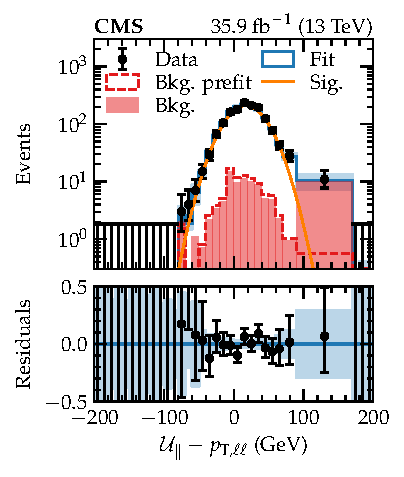
\includegraphics{chapters/041_corrections/images/ptmiss_calib/metres_datafit_example.pdf}
        \caption{Data fit}
        \label{subfiga:metres-fit-examples}
    \end{subfigure}
    \begin{subfigure}[b]{0.49\textwidth}
        \centering
        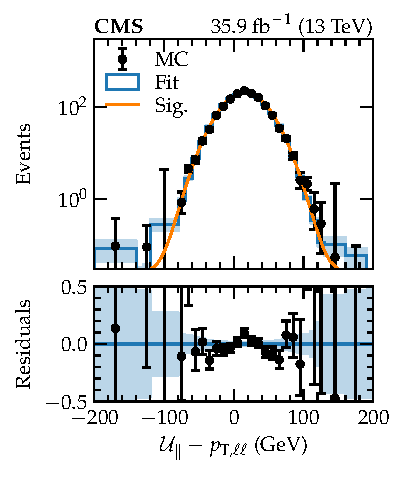
\includegraphics{chapters/041_corrections/images/ptmiss_calib/metres_mcfit_example.pdf}
        \caption{MC fit}
        \label{subfigb:metres-fit-examples}
    \end{subfigure}
    \caption[Fit result to extract the recoil scale and resolution in data and simulation.]{
        Fit results for the \IDYmm process in \ptll bin $180$--$\SI{190}{GeV}$ in data and MC; showing the fit result, background (Bkg.) prefit and postfit, signal Voigtian (Sig.) and the total fit result and it's uncertainty band; for the $\mathcal{U}_{\parallel}-\ptll$ distribution. The merging of bins is apparent with the wide bin where the background estimation increases by a factor of 10 as a result of large event weights leading to low effective MC statistics with this wide bin. The residuals represent the difference between the data points and the fit result with good agreement in the data fit and slightly worse in the MC fit as systematic uncertainties are not included to cover the discrepancy.
    }
    \label{fig:metres-fit-examples}
\end{figure}

The scale $u_0$ and resolution $\sigma_V$ extracted from the fits for each \ptll bin is shown in Fig.~\ref{fig:recoil-calib-ptllbins-mm} for the \dimuplusjets region and Fig.~\ref{fig:recoil-calib-ptllbins-ee} for the \dieleplusjets region.
%
\begin{figure}[htb]
    \centering
    \begin{subfigure}[b]{0.49\textwidth}
        \centering
        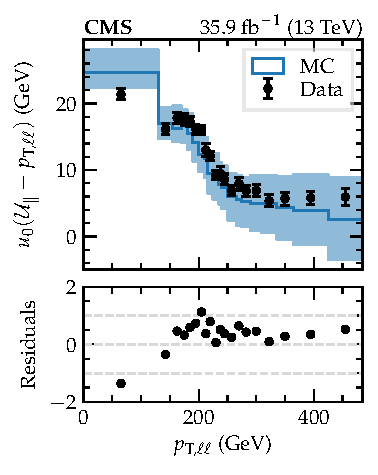
\includegraphics{chapters/041_corrections/images/ptmiss_calib/metres_mm_u0_para.pdf}
        \caption{Parallel scale}
        \label{subfiga:recoil-calib-ptllbins-mm}
    \end{subfigure}
    \hfill
    \begin{subfigure}[b]{0.49\textwidth}
        \centering
        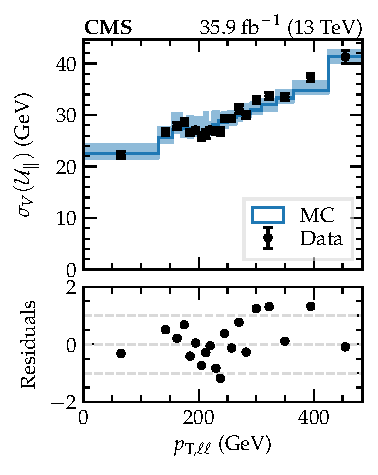
\includegraphics{chapters/041_corrections/images/ptmiss_calib/metres_mm_sigmav_para.pdf}
        \caption{Parallel resolution}
        \label{subfigb:recoil-calib-ptllbins-mm}
    \end{subfigure}
    \\
    \begin{subfigure}[b]{0.49\textwidth}
        \centering
        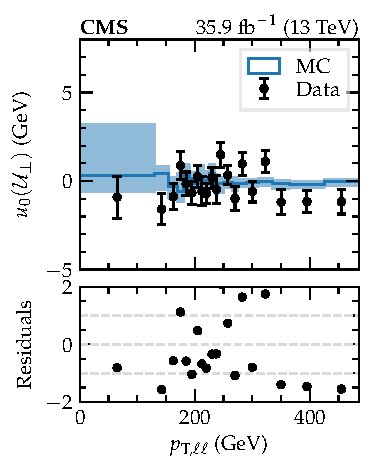
\includegraphics{chapters/041_corrections/images/ptmiss_calib/metres_mm_u0_perp.pdf}
        \caption{Perpendicular scale}
        \label{subfigc:recoil-calib-ptllbins-mm}
    \end{subfigure}
    \hfill
    \begin{subfigure}[b]{0.49\textwidth}
        \centering
        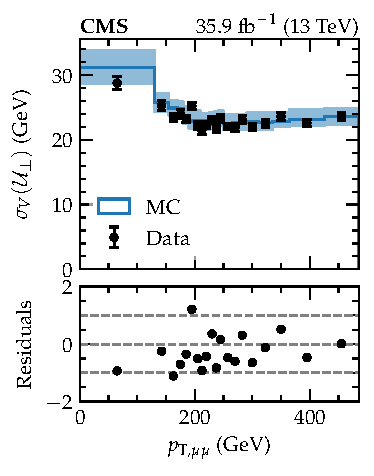
\includegraphics{chapters/041_corrections/images/ptmiss_calib/metres_mm_sigmav_perp.pdf}
        \caption{Perpendicular resolution}
        \label{subfigd:recoil-calib-ptllbins-mm}
    \end{subfigure}
    \caption[Recoil scale and resolution in the dimuon final state.]{
        The \ptmiss scale and resolution from the fit to data and MC in the \dimuplusjets region. The residuals represent the difference between data and MC, scaled by the reciprocal of the uncertainties added in quadrature.
    }
    \label{fig:recoil-calib-ptllbins-mm}
\end{figure}
%
\begin{figure}[htb]
    \centering
    \begin{subfigure}[b]{0.49\textwidth}
        \centering
        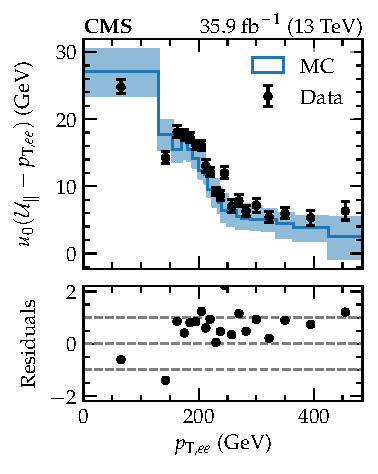
\includegraphics{chapters/041_corrections/images/ptmiss_calib/metres_ee_u0_para.pdf}
        \caption{Parallel scale}
        \label{subfiga:recoil-calib-ptllbins-ee}
    \end{subfigure}
    \hfill
    \begin{subfigure}[b]{0.49\textwidth}
        \centering
        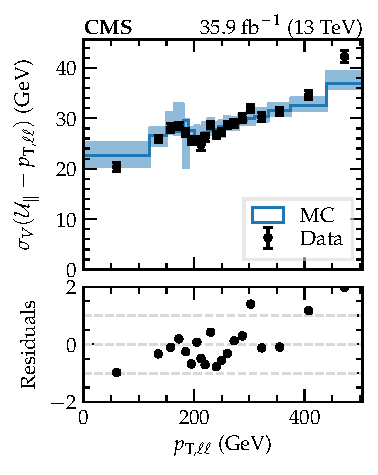
\includegraphics{chapters/041_corrections/images/ptmiss_calib/metres_ee_sigmav_para.pdf}
        \caption{Parallel resolution}
        \label{subfigb:recoil-calib-ptllbins-ee}
    \end{subfigure}
    \\
    \begin{subfigure}[b]{0.49\textwidth}
        \centering
        \includegraphics{chapters/041_corrections/images/ptmiss_calib/metres_ee_u0_perp.pdf}
        \caption{Perpendicular scale}
        \label{subfigc:recoil-calib-ptllbins-ee}
    \end{subfigure}
    \hfill
    \begin{subfigure}[b]{0.49\textwidth}
        \centering
        \includegraphics{chapters/041_corrections/images/ptmiss_calib/metres_ee_sigmav_perp.pdf}
        \caption{Perpendicular resolution}
        \label{subfigd:recoil-calib-ptllbins-ee}
    \end{subfigure}
    \caption[Recoil scale and resolution in the dielectron final state.]{
        Similar results to Fig.~\ref{fig:recoil-calib-ptllbins-mm} in the \dieleplusjets region.
    }
    \label{fig:recoil-calib-ptllbins-ee}
\end{figure}
%
The scale and resolution in both the \dimuplusjets and \dieleplusjets region agree within their respective uncertainties. Therefore, no additional corrections are derived for the scale or the resolution since the recoil as a proxy for the boson \pt is well-modelled in MC. A few outliers with residuals beyond $\pm 1$ are seen; however, the number is not significantly beyond expectations given the number of bins probed. Furthermore, the most important parameter, the parallel scale, shows an overestimate in the systematic uncertainties.

Additional studies into the recoil calibration with the number of pileup vertices have been performed elsewhere \cite{Sirunyan:2019kia} and show good agreement between data and MC.

\clearpage
\section{Summary}

Corrections are applied to simulation to improve the modelling of data, typically determined from data-driven measurements of scale factors to correct the efficiency of a selection in MC to match the data efficiency, along with systematic uncertainties representing limitations in the scale factors.

The first set of corrections fix the emulated trigger efficiency in MC for the single muon and electron trigger paths measured in \IDYll events with the tag and probe method. The \ptmiss trigger scale factors are determined from events collected by the single muon trigger paths as a reference. Systematic uncertainties estimate the effect of the muon mismatch between the \SWT and offline selection, the use of the single muon trigger reference and variations from an independent region. After the trigger corrections are applied, object based selection corrections are measured, typically with the tag and probe method, for the muon identification and isolation; electron identification, isolation and reconstruction; photon identification and track veto; and jet $b$ and \Ptauh-tag identification.  Similarly, the energy and \pt scale corrections and systematic uncertainties are measured for muons, \Ptauh, electrons, photons and jets, all of which are propagated through the recoil calculation. Global event-based corrections and uncertainties are determined for the luminosity measurement, pileup reweighting, ECAL timing degradation and theory corrections to higher precision in QCD and electroweak vertices including QCD factorisation and renormalisation scale and PDF variations. The use of the recoil variable as a proxy for the boson \pt in \IZvvj, \IWlvj and \IDYllj processes is probed in \IDYllj events by splitting the recoil into a parallel and perpendicular component to extract the scale and resolution in both data and MC. The results show good agreement, within uncertainties, hence no additional corrections or systematic uncertainties are required.

All corrections are applied to the relevant processes in simulated events. Alternative distributions are provided under the $\pm 1\sigma$ variations for later likelihood fits to extract the \IZvvj and \IZllj event yields in determining the \PZ invisible width.

        \chapter{Background estimation}
\label{chap:backgrounds}

%\chapterquote{}{}

\section{Introduction}

The processes used to extract the \PZ invisible width are \IZvv and \IZll. The \IZll process is selected by the \dimuplusjets and \dieleplusjets regions and receives small contributions from background processes, predominantly diboson, as a result of the signal enhancement from the invariant mass selection. Therefore, these backgrounds are estimated from MC after the corrections discussed in Chap.~\ref{chap:simulation-corrections} are applied. Furthermore, the distinction between the \IDYll and \IZll processes requires an estimate of the contribution of the \Pgstar background as well as the interference between \PZ and \Pgstar. With the invariant mass selection, the \Pgstar and interference contributions are percent-level and hence estimated directly from MC simulations where the \PZ and \Pgstar contributions are subsequently turned off in the event generation. Meanwhile, the \IZvv process is collected in the \metplusjets region which is contaminated by the \IWlv decay where the lepton is out of acceptance or a misidentified \Ptauh.  This \IWlv background is estimated by a data-driven control region method. The remaining backgrounds are significantly smaller and estimated from MC, apart from the QCD multijet background which, although small, is estimated with a data-driven method because of large uncertainties associated with the QCD multijet prediction in MC. All these estimation methods are discussed in this chapter.

The estimation methods are performed in orthogonal control regions to the \metplusjets and \diellplusjets signal regions. However, decisions on further categorisation within the regions is closely aligned to the signal regions.  Although the determination of the \PZ invisible width requires the overall event yield for the \IZvv and \IZll processes, the \recoil is divided into bins to exploit the background and systematic uncertainty dependence on this parameter. The chosen bin widths are approximately equivalent to the resolution of the \recoil with an open-ended final bin, as detailed in Tab.~\ref{tab:met-bins}.

\begin{table}[htb]
    \centering
    \begin{tabular}{ccccccc}
        $200$--$220$ & $220$--$250$ & $250$--$280$ & $280$--$310$ & $310$--$340$ & $340$--$370$ & $370$--$400$ \\
        $400$--$430$ & $430$--$470$ & $470$--$510$ & $510$--$550$ & $550$--$590$ & $590$--$640$ & $640$--$690$ \\
        $690$--$740$ & $740$--$790$ & $790$--$840$ & $840$--$900$ & $900$--$960$ & $960$--$1020$ & $1020$--$1090$ \\
        $1090$--$1160$ & $1160$--$1250$ & $1250$--$1400$ & $1400$--$\inf$
    \end{tabular}
    \caption[Recoil bins.]{
        Division of the recoil, in GeV, into 25 bins for the background estimation and \PZ invisible width extraction. Exploiting the shape of the recoil distribution exposes regions with larger signal to background ratios and various systematic uncertainty contributions.
    }
    \label{tab:met-bins}
\end{table}

\section{\IWlv prediction}\label{sec:wjets-prediction}

The \IWlv process contribution in the \metplusjets region is estimated from an orthogonal control region defined by the reconstruction and selection of a single lepton, rather than vetoing all leptons. Two control regions are defined: the \muplusjets and \eleplusjets, both are used in this estimation method as a source of well-reconstructed leptons and complement each other.  These regions are linked to the \metplusjets region through the transfer factor method, discussed in the following section. In addition to the two control regions, the \tauplusjets is defined as a validation region to test the use of muon and electron final states to primarily predict the $\tau$-lepton decay of the \IWlv process.


\subsection{\muplusjets control region}

The \muplusjets control region provides the primary measurement for the data-driven estimate of \IWlv in the \metplusjets region. It differs from this region by requiring a single well-reconstructed muon in the final state along with a transverse invariant mass between the muon and the \ptmiss between $30$ and $\SI{125}{GeV}$. The kinematic distributions for this region are shown in Fig.~\ref{fig:muplusjets}.
%
\begin{figure}[htb]
    \centering
    \includegraphics{chapters/042_backgrounds/images/singlemuon_dists.pdf}
    \caption[Single muon final state kinematics.]{
        Distributions of kinematic variables within the \muplusjets region. The ratio of data to MC is shown in the lower sub-panels along with the statistical uncertainty associated with the MC prediction, without any systematic uncertainties. Processes with the largest cross sections are labelled with a grouping of the smallest contributions into the `minor' background.
    }
    \label{fig:muplusjets}
\end{figure}
%
The most prominent processes include the signal of interest, \IWmvj ($82.1\%$), along with backgrounds from: \IWlv with a $\tau$-lepton decaying into a muon ($5.4\%$); $t$-quark production ($5.3\%$) and subsequent decay into a muon, jets and neutrinos; diboson production ($2.0\%$); Drell-Yan production of dimuons ($2.0\%$) with one muon out of acceptance or misreconstructed; QCD multijet ($1.3\%$) and other processes ($1.9\%$). The shape of the data and MC distributions are in agreement. Dependence, for instance, with the lead muon $\eta$ is covered by systematic uncertainties which are larger in the endcaps where the particle flux is greater and the magnetic field is more complex. However, there is a significant discrepancy of $10\%$ between the data and MC normalisation, currently attributed to a normalisation issue with the \IWj production\footnote{This issue has been identified as a problematic cross section deviating from the true theory prediction by about $10\%$ across the full boson \pt range for the \IWj process.}. The analysis is designed to be robust against incorrect normalisations with the \IVj process through data-driven measurements. This is investigated further by inspecting the \eleplusjets control region.


\subsection{\eleplusjets control region}

The selection for the \eleplusjets control region is closely aligned to the \muplusjets to provide a complementary measurement of the \IWlvj process. However, the additional selection ${\ptmiss>\SI{100}{GeV}}$ reduces QCD multijet contamination within this region and the statistical power to measure the \IWlvj process. The kinematic distributions of this region are shown in Fig.~\ref{fig:eleplusjets} where the same $10\%$ discrepancy between the normalisation in data and MC is observed, although the shapes of the distributions are in good agreement.
%
\begin{figure}[htb]
    \centering
    \includegraphics{chapters/042_backgrounds/images/singleele_dists.pdf}
    \caption[Single electron final state kinematics.]{
        Kinematic variable distributions of the \eleplusjets control region. The ratio of data to MC gives an indication of their agreement within statistical uncertainties on both the data and MC. However, no systematic uncertainties are included. The most prominent processes are the electron ($81.1\%$) and $\tau$-lepton ($7.4\%$) decays of the \PW boson, with subsequently smaller contributions from $t$-quark production ($6.6\%$) and other `minor' backgrounds which include diboson, \IDYee and QCD multijet processes. The asymmetry in the lead electron $\eta$ is covered by electron identification uncertainties which are significantly larger in the forward $\eta$ regions.
    }
    \label{fig:eleplusjets}
\end{figure}
%
Therefore, the normalisation is not attributed to the muon or electron reconstruction and identification or the trigger since they differ for the \muplusjets and \eleplusjets regions. This supports the original hypothesis of a normalisation issue with the \IWj process. Under this hypothesis the normalisation is expected to persist into the \metplusjets region, scaled down by the relative contribution of the \IWj process. Therefore, the data-driven estimate of this process is vital for an accurate background prediction. The \tauplusjets region is explored to further support or refute this hypothesis. The different background composition compared to Fig.~\ref{fig:muplusjets} is driven by the additional \ptmiss selection in the \eleplusjets region.


\subsection{\tauplusjets validation region}

The \tauplusjets validation region is more aligned with the \metplusjets region than the \muplusjets or \eleplusjets control regions since no well-reconstructed lepton exists in the final state, instead a hadronic cluster is tagged as the decay product of a $\tau$-lepton. However, as shown in Fig.~\ref{fig:tauplusjets}, this region receives a substantial contribution from other hadronic final states with jets mistagged as a \Ptauh and a lower sample size due to the \Ptauh-tagging efficiency with a large associated uncertainty.
%
\begin{figure}[htb]
    \centering
    \includegraphics{chapters/042_backgrounds/images/singletau_dists.pdf}
    \caption[Single hadronic $\tau$-lepton final state kinematics.]{
        Kinematic distributions for the \tauplusjets validation region. The \IWj process is dominant with the $\tau$-lepton ($73.4\%$) and electron ($6.9\%$) decays, with subsequently smaller backgrounds from $t$-quark production ($5.7\%$); QCD multijet ($3.6\%$); diboson production ($3.2\%$); vector boson scattering, VBS ($1.8\%$); and other contributions grouped into the `minor' background.
    }
    \label{fig:tauplusjets}
\end{figure}
%
Therefore, for the purpose of measuring the \IWj process, the \tauplusjets region does not provide a similar precision to the \muplusjets and \eleplusjets regions. However, as a validation region it supports the normalisation offset associated with the \IWj process at $8\%$, with the shapes of the kinematic distribution in good agreement, within uncertainties, between data and MC.


\subsection{Systematic uncertainties}\label{sec:systs}

The \IWj background estimation is based on a data-driven estimate to improve the MC prediction. The systematic uncertainties associated with the MC predictions, most notably from limited knowledge of selection efficiencies, impact this estimation. The full set of systematic uncertainties affecting the background estimation is as follows.

\begin{itemize}
    \item All \textbf{theory uncertainties} discussed in Sec.~\ref{sec:theory-corrections}.
    \item \textbf{Veto efficiencies} associated to uncertain corrections in vetoing $b$-jets, photons and \Ptauh-leptons. The photons have two associated uncertainties: identification and pixel seed veto efficiencies.
    \item \textbf{Proton beam uncertainties} such as the luminosity measurement ($\SI{2.5}{\%}$) and the pileup profile.
    \item \textbf{Detector-based uncertainties} due to online issues whilst recording data. The most significant uncertainty is due to the ECAL timing issue.
    \item \textbf{Trigger efficiencies} as described in Sec.~\ref{sec:met-trigger-efficiency} and \ref{sec:electron-trigger-efficiency}. The \ptmiss trigger efficiency uncertainty is split into three sources: reference trigger, muon multiplicity and independent region. The reference trigger uncertainty is correlated between all regions whereas the muon multiplicity is split into the $0\ \mu$, $1\ \mu$ and $2\ \mu$ regions and the independent region systematic is uncorrelated between all regions.
    \item \textbf{Muon efficiency uncertainties} associated to veto and selection muon identification and isolation with an uncorrelated statistical and systematic component.
    \item \textbf{Electron efficiency uncertainties} associated to veto and selection electron identification and reconstruction.
    \item \textbf{Jet energy correction uncertainties} determined by varying the scale (JES) and resolution (JER) of jet energies.
    \item \textbf{Unclustered energy uncertainty} encoding the impact of energy deposits, below the clustering threshold, on \ptmiss.
\end{itemize}


\subsection{Transfer factor method}

The transfer factor method is based on applying correction factors, determined from control regions, to improve background predictions in a signal region whilst reducing the systematic uncertainties associated with this estimation.  The \IWj prediction in the \metplusjets region, $N_{\mathrm{pred}}^{\metplusjets}(\IWj)$, is determined from the \ellplusjets regions as
%
\begin{equation}
    N_{\mathrm{pred}}^{\metplusjets}(\IWj) = \frac{N_{\mathrm{MC}}^{\metplusjets}(\IWj)}{N_{\mathrm{MC}}^{\ellplusjets}(\IWj)} \left(N_{\mathrm{obs}}^{\ellplusjets} - N_{\mathrm{MC}}^{\ellplusjets}(\mathrm{bkgs.})\right)\ ,
\end{equation}
%
where $N_{\mathrm{MC}}^{\metplusjets}(\IWj)$ and $N_{\mathrm{MC}}^{\ellplusjets}(\IWj)$ are the MC predictions for the \IWj process in the \metplusjets and \ellplusjets regions, respectively; $N_{obs}^{\ellplusjets}$ is the observed number of events in data for the \ellplusjets regions, and $N_{\mathrm{MC}}^{\ellplusjets}(\mathrm{bkgs.})$ is the MC prediction for the backgrounds (processes other than \IWj) in the \ellplusjets region. The transfer factor is given by the ratio
%
\begin{equation}
    t_{\ellplusjets}^{\metplusjets}(\IWj) = \frac{N_{\mathrm{MC}}^{\metplusjets}(\IWj)}{N_{\mathrm{MC}}^{\ellplusjets}(\IWj)}\ .
\end{equation}
%
Systematic uncertainties common in both the numerator and denominator typically cancel, reducing the systematic uncertainty associated with the transfer factor, with respect to the individual MC predictions. In practice, the transfer factor method is implemented within the likelihood formalism (App.~\ref{app:likelihood}) by scaling the \IWj process in the signal and control regions by a common unconstrained parameter $r_{\PW}$ determined from a simultaneous fit to the data in the \metplusjets and \ellplusjets region. Here, the likelihood is given by the product over all \recoil bins with two poisson terms for the \metplusjets and \ellplusjets region with the expectation values
%
\begin{equation}
    r_{\PZ}s_{\IZvv}^{\metplusjets}(\bm{\theta},\phi^{\metplusjets})%
    + r_{\PW}s_{\IWlv}^{\metplusjets}(\bm{\theta},\phi^{\muplusjets})%
    + b^{\metplusjets}(\bm{\theta},\phi^{\metplusjets})
\end{equation}
%
and
%
\begin{equation}\label{eq:ellplusjets-expectation}
    r_{\PW}s_{\IWlv}^{\ellplusjets}(\bm{\theta},\phi^{\ellplusjets})%
    + b^{\ellplusjets}(\bm{\theta},\phi^{\ellplusjets})\ ,
\end{equation}
%
respectively. The \IZvv contribution in the \metplusjets region, $s_{\IZvv}$, is scaled by the parameter of interest $r_{\PZ}$; and similarly by $r_{\PW}$ for the \IWlv process $s_{\IWlv}$. The remaining backgrounds, $b$, and all other processes depend on the gaussian constrained, $\bm{\theta}$, and poisson constrained MC statistical, $\phi$, nuisance parameters. Superscripts denote the parameter's associated region. The scaling parameters $r_\PZ$ and $r_\PW$ are correlated across all \recoil bins, and estimated from a fit to the data. Prior to the fit the MC predictions and the transfer factors are inspected, as shown in Fig.~\ref{fig:tfs_emu_sr}.

\begin{figure}[htb]
    \centering
    \begin{subfigure}[b]{\textwidth}
        \centering
        \includegraphics{chapters/042_backgrounds/images/tf_mu_sr.pdf}
        \caption{Transfer factor for \IWj from the \muplusjets to \metplusjets region.}
        \label{subfiga:tfs_emu_sr}
    \end{subfigure}
    \\
    \begin{subfigure}[b]{\textwidth}
        \centering
        \includegraphics{chapters/042_backgrounds/images/tf_e_sr.pdf}
        \caption{Transfer factor for \IWj from the \eleplusjets to \metplusjets region.}
        \label{subfigb:tfs_emu_sr}
    \end{subfigure}
    \caption[Muon and electron transfer factors into the signal region]{
        Distributions of the \recoil variable in the \muplusjets, \eleplusjets and \metplusjets with the transfer factor determined from the \IWj MC estimates. The transfer factor includes the uncertainties associated with the limited number of generated MC events and systematic uncertainties from all sources whereas the kinematic distributions only include the statistical uncertainties. The distributions also include the analysis relevant processes.
    }
    \label{fig:tfs_emu_sr}
\end{figure}

The transfer factor is a steeply falling distribution where leptons from \PW decays are more likely to be below the \pt acceptance, misreconstructed or misidentified with a lower recoil. However, the \pt of the lepton increases with the recoil and is significantly harder to miss, resulting in the transfer factor tending to zero. Furthermore, the transfer factor is larger for the \eleplusjets predictor rather than \muplusjets because of the tighter selection and lower reconstruction efficiency associated with the electrons.

The systematic uncertainties associated with the \muplusjets and \eleplusjets transfer factor are split into the theoretical and experimental uncertainties. The relative systematic uncertainties associated with the transfer factor $t_{\muplusjets}^{\metplusjets}(\IWj)$ and $t_{\eleplusjets}^{\metplusjets}(\IWj)$ are shown in Figs.~\ref{fig:tf-systs-muplusjets-1}--\ref{fig:tf-systs-eleplusjets-2}, with the uncertainties prior to the transfer factor shown in App.~\ref{appsec:alt_temp}.
%
\begin{figure}
    \centering
    \includegraphics{chapters/042_backgrounds/images/tf_wj_mu_met_systs1.pdf}
    \caption[Theoretical uncertainty on the transfer factors]{
        Relative systematic uncertainties (\%) on the \IWj transfer factor for the \metplusjets region predicted by the \muplusjets control region. The uppermost panel includes all the theoretical uncertainties, while the others include experimental uncertainties. The total uncertainty, depicted in each panel, represents all uncertainties summed in quadrature.
    }
    \label{fig:tf-systs-muplusjets-1}
\end{figure}
%
\begin{figure}
    \centering
    \includegraphics{chapters/042_backgrounds/images/tf_wj_mu_met_systs2.pdf}
    \caption[Object-based uncertainties on the transfer factors]{
        Additional object-based systematic uncertainties to Fig.~\ref{fig:tf-systs-muplusjets-1}.
    }
    \label{fig:tf-systs-muplusjets-2}
\end{figure}
%
\begin{figure}
    \centering
    \includegraphics{chapters/042_backgrounds/images/tf_wj_ele_met_systs1.pdf}
    \caption[Theoretical uncertainty on the transfer factors]{
        Relative systematic uncertainties (\%) on the \IWj transfer factor for the \metplusjets region predicted by the \eleplusjets control region. The uppermost panel includes all the theoretical uncertainties, while the others include experimental uncertainties. The total uncertainty, depicted in each panel, represents all uncertainties summed in quadrature.
    }
    \label{fig:tf-systs-eleplusjets-1}
\end{figure}
%
\begin{figure}
    \centering
    \includegraphics{chapters/042_backgrounds/images/tf_wj_ele_met_systs2.pdf}
    \caption[Object-based uncertainties on the transfer factors]{
        Additional object-based systematic uncertainties to Fig.~\ref{fig:tf-systs-eleplusjets-1}.
    }
    \label{fig:tf-systs-eleplusjets-2}
\end{figure}
%
The theoretical uncertainties primarily cancel as they affect the \IWj process equally in the \metplusjets and \muplusjets regions. However, the parton distribution function (PDF) uncertainty does not completely cancel as different partons initiate the interaction as a result of kinematic sculpting by requirements on muon \pt and $\eta$ which are not applied in the \metplusjets region. Nevertheless, these contributions are small in comparison to the experimental uncertainties. The dominant systematic uncertaintes include the jet energy scale, $\Ptauh$-tag veto efficiency and pileup reweighting uncertainty with large contributions from the \ptmiss trigger efficiency for ${\recoil<\SI{250}{GeV}}$. The alternative templates representing the $\pm 1\sigma$ variations in the jet energy scale uncertainty are statistically limited in their precision, whereas they are assumed to be precise within the likelihood fit, leading to non-cancellations in the transfer factor. To partially redeem this issue the alternative templates are smoothed in an attempt to remove statistical fluctuations (App.~\ref{app:likelihood}). Although this proves to be beneficial in obtaining a good fit to the data the resulting uncertainty is typically dominated by the limited MC sample size.

A set of validation studies are performed to test the transfer factor and the extrapolation involved in predicting the \IWj process in the \metplusjets regions from the \IWj process in the \ellplusjets region.


\subsection{Validation}

Several aspects of the transfer factor approach are tested to determine if additional systematic uncertainties are required to cover mismodelling, undercoverage or bias in the MC prediction. The major background in the \metplusjets region consists of the \IWj process ($34.7\%$), split by decay mode: electron ($6.3\%$), leptonic decay of the $\tau$-lepton ($6.9\%$), muon ($9.2\%$) and \Ptauh-lepton ($12.3\%$). The data-driven estimate of these processes is performed from the \muplusjets and \eleplusjets control regions.  The leptonic decay of the $\tau$-lepton is similar to the electron and muon decay modes, with a typically broader \recoil distribution. However, the \Ptauh-lepton decay mode differs by being a fully hadronic final state.  Therefore, the validation tests are as follows: test the grouping of the muon and electron decay modes, test the extrapolation of the muon and electron decay modes to predict the \Ptauh-lepton decay mode, and a test of the effects of \PW polarisation.

The first test verifies the consistency of the \muplusjets and \eleplusjets region to validate their combination in measuring the \IWj process. A simultaneous likelihood fit is performed between both regions with expected values given by Eq.~\ref{eq:ellplusjets-expectation}. Two additional unconstrained parameters are applied to the \IWj prediction in the \eleplusjets region to extract the normalisation, $r_e$, and shape, $\beta_e$, difference between both regions. Therefore, the expectation for the \IWj process in the \eleplusjets region is modified to
%
\begin{equation}
    r_{\PW}s_{\IWlv}^{\eleplusjets}\mapsto \left(r_e + \beta_{e}(\recoil/\langle\recoil\rangle-1)\right)r_{\PW}s_{\IWlv}^{\eleplusjets}\ ,
\end{equation}
%
where $\langle \mathcal{U} \rangle$ is the weighted average of the \recoil distribution to scale $\beta_e$ to a dimensionless parameter, $\beta_e$ varies the shape of the \IWj process in the \eleplusjets region linearly with respect to the \muplusjets region. Perfect consistency between both regions corresponds to $r_e=1$ and $\beta_e=0$. The postfit\footnote{Postfit refers to the set of best fit values, or parameters determined at these values, estimated from a fit to the data. Conversely, prefit refers to the set of initial values, prior to a fit to the data. The values are typically chosen such that the prefit distributions correspond to the MC predictions.} values for the parameters of interest are
%
\begin{align}
    r_e & = 0.95^{+0.05}_{-0.05}\qquad \mathrm{and}\nonumber\\
    \beta_e & = -0.020^{+0.024}_{-0.023}\ .
\end{align}
%
Both are in agreement with a consistent muon and electron channel. The quality of the fit is inspected through the postfit results for the nuisance parameters along with their impact on the parameter of interest $r_e$, shown in Fig.~\ref{fig:fit_tf_mu_e_wj_impacts}.
%
\begin{figure}[htb]
    \centering
    \includegraphics{chapters/042_backgrounds/images/impacts_tfmu2ewj.pdf}
    \caption[Nuisance parameters from a simultaneous fit to the muon and electron control regions]{
        Result of a simultaneous fit between the \muplusjets and \eleplusjets region to extract the scale and shape difference between the muon and electron decay modes. The postfit values for the nuisance parameters and their uncertainties are shown as $\theta$ as well as the impact of fixing the nuisance parameters at the $+1\sigma$ and $-1\sigma$ values to determine the effect on the parameter of interest, $\Delta \hat{r}_e$. The set of parameters is restricted to the top $15$, in order of impact on the parameter of interest. The $\theta$ value for $r_e$ is omitted since it is not a nuisance parameter, instead it is included as a reference for its uncertainty shown in $\Delta \hat{r}_e$.
    }
    \label{fig:fit_tf_mu_e_wj_impacts}
\end{figure}
%
The postfit nuisance parameters are within a satisfactory limit without significant deviations from the $|\theta|<1$ region. Therefore, discrepancies between the data and prediction are covered by the unconstrained parameters, with a slight deviation in the low recoil \muplusjets region covered by the \ptmiss trigger efficiency systematic. The systematic uncertainties with the largest impact on the scale $r_e$ are the electron identification, trigger and reconstruction efficiency uncertainties. The postfit distributions, Fig.~\ref{fig:fit_tf_mu_e_wj_postfit}, show the consistency between the postfit prediction and the data.
%
\begin{figure}[htb]
    \centering
    \includegraphics{chapters/042_backgrounds/images/postfit_tfmu2ewj.pdf}
    \caption[Recoil distributions in the muon and electron control regions after applying the transfer factors]{
        Distributions of the \recoil in the \muplusjets and \eleplusjets with the prefit inputs as well as the postfit results along with its uncertainty. The upper panel shows the results in terms of the event counts with the postfit background composition, while the middle panel shows the ratio to the postfit value and the residuals are defined by the difference between the data and postfit result, normalised by the statistical and systematic uncertainties summed in quadrature.
    }
    \label{fig:fit_tf_mu_e_wj_postfit}
\end{figure}
%
A good agreement between the data and postfit values supports the results of the fit and the consistency of the \muplusjets and \eleplusjets. Therefore, the current \IWj prediction formed from a mixture of muon and electron decay modes is kept without the need for additional systematic uncertainties to cover further mismodelling, even though the selections and background compositions differ.

The next validation is a test of the consistency between the \muplusjets and \eleplusjets with the \tauplusjets region. This probes the extrapolation performed by the transfer factor method, using the \muplusjets and \eleplusjets region to predict the \IWj process in the \metplusjets region which mostly consists of \Ptauh decays of the \PW boson. This test is performed in a similar way to the previous test, however, the \IWj process in the \muplusjets and \eleplusjets regions are scaled by a single unconstrained parameter $r_W$, whereas the equivalent process in the \tauplusjets region is scaled by
%
\begin{equation}
    \left(r_\tau + \beta_\tau (\mathcal{U}/\langle \mathcal{U} \rangle - 1)\right) r_\PW s_{\IWlv}^{\tauplusjets}\ .
\end{equation}
%
The postfit values of these parameters are
%
\begin{align}
    r_\tau & = 1.04^{+0.07}_{-0.06}\qquad\mathrm{and} \nonumber\\
    \beta_\tau & = -0.008^{+0.046}_{-0.047}\ .
\end{align}
%
Again, these values show a consistency in the shape and normalisation of the \ellplusjets and \tauplusjets channels. The nuisance parameters and their impacts on the parameter of interest $r_\tau$ is shown in Fig.~\ref{fig:fit_tf_mue_t_wj_impacts}.
%
\begin{figure}[htb]
    \centering
    \includegraphics{chapters/042_backgrounds/images/impacts_tfmue2twj.pdf}
    \caption[Nuisance parameters from a fit with the transfer factor method from the muon and electron control regions to the $\tau$-lepton validation region.]{
        Postfit nuisance parameters and impact on $r_\tau$ from a simultaneous fit between the \muplusjets, \eleplusjets and \tauplusjets region. The format is aligned with Fig.~\ref{fig:fit_tf_mu_e_wj_impacts}.
    }
    \label{fig:fit_tf_mue_t_wj_impacts}
\end{figure}
%
Although the \tauplusjets suffers from a smaller sample size compared to the \muplusjets and \eleplusjets regions, the most dominant source of uncertainty comes from the \Ptauh-tag identification uncertainty, albeit unsurprisingly.  The pull\footnote{A pull on a postfit nuisance parameter refers to the deviation of the postfit value from its prefit.} on the \ptmiss trigger efficiency is consistent with the first test since the same region is used, with an enhanced pull on the PDF uncertainties, although within the satisfactory region. The associated \recoil distributions from this fit are shown in Fig.~\ref{fig:fit_tf_mue_t_wj_postfit}.
%
\begin{figure}[htb]
    \centering
    \includegraphics{chapters/042_backgrounds/images/postfit_tfmue2twj.pdf}
    \caption[Recoil distributions corrected by the transfer factor from the muon and electron control regions to the $\tau$-lepton validation region.]{
        Recoil distributions for the \muplusjets, \eleplusjets and \tauplusjets region from a fit to the data to test the extrapolation of a well-reconstructed muon or electron to predict the rate of \Ptauh decays from the \IWj process. The axis definitions are aligned with Fig.~\ref{fig:fit_tf_mu_e_wj_postfit}.
    }
    \label{fig:fit_tf_mue_t_wj_postfit}
\end{figure}
%
The \muplusjets and \eleplusjets regions are similar to those shown in Fig.~\ref{fig:fit_tf_mu_e_wj_postfit} because the \tauplusjets region does not provide any additional information. Furthermore, the data and postfit result in the \tauplusjets region are in excellent agreement. This is partially by design from the unconstrained parameters $r_\tau$ and $\beta_\tau$ used to extract the consistency between the various channels.

The final validation tests the extrapolation performed from the different admixture of $\PW^{\pm}$ polarisation states between the \ellplusjets and \metplusjets regions. The different admixture is a result of the typically softer $\ell^+$ \pt compared to $\ell^-$ \pt to maintain the left-handed chiral state of the associated neutrino (and right-handed anti-neutrino) \cite{Bern:2011ie}. This validation is performed with a similar method, however, the \muplusjets is split into two regions: $\mu^- +\mathrm{jets}$ is used to predict the \IWj process in the $\mu^+ + \mathrm{jets}$, hence testing this extrapolation. Since the admixture difference is significantly smaller than the difference between these two regions, any result discrepancies will have a reduced impact on the \IWj prediction. In this fit, both regions are scaled by the unconstrained parameter $r_\PW$, with two additional normalisation and shape parameters applied to the $\mu^+ +\mathrm{jets}$ region as
%
\begin{equation}
    \left(r_{\mu^+} + \beta_{\mu^+}(\mathcal{U}/\langle\mathcal{U}\rangle-1)\right)r_\PW s_{\IWlv}^{\mu^++\mathrm{jets}}\ .
\end{equation}
%
The postfit values for the parameters from a fit to the data are
%
\begin{align}
    r_{\mu^+} & = 0.976^{+0.013}_{-0.013}\qquad\mathrm{and}\nonumber\\
    \beta_{\mu^+} & = 0.007^{+0.025}_{-0.024}\ .
\end{align}
%
The uncertainty on the normalisation parameter is noticeably smaller than previous validation tests as a result of the closer alignment between both regions leading to further cancellations with the transfer factor method. The null hypothesis of consistent shape and normalisation between the \mupplusjets and \munplusjets is within the $95\%$ confidence level\footnote{A null hypothesis is typically excluded if it falls outside of the $95\%$ confidence interval.} with an excellent shape agreement and a normalisation near the boundary, although within the consistent limits. The postfit nuisance parameters and their impacts on the unconstrained parameter $r_{\mu^+}$ are shown in Fig.~\ref{fig:fit_tf_mup_mun_wj_impacts}.
%
\begin{figure}[htb]
    \centering
    \includegraphics{chapters/042_backgrounds/images/impacts_tfmup2munwj.pdf}
    \caption[Nuisance parameters from a fit to the positive and negative muon control regions.]{
        Postfit nuisance parameters from a simultaneous fit to the \mupplusjets and \munplusjets regions to extract the shape and normalisation difference. The impacts on the $r_{\mu^+}$ parameter are shown. The format is aligned with Fig.~\ref{fig:fit_tf_mu_e_wj_impacts}. The enhanced postfit uncertainty on the jet energy resolution is a result of its asymmetric uncertainties evident from its $\Delta \hat{r}_{\mu^+}$ impact.
    }
    \label{fig:fit_tf_mup_mun_wj_impacts}
\end{figure}
%
The pulls are consistent with previous results including the \muplusjets region, without any significant deviations from the prefit values. No significant constraints are estimated for the nuisance parameters, other than a slight constraint on the $\delta^{(2)}k_{\mathrm{QCD}}$, also seen in Fig.~\ref{fig:fit_tf_mu_e_wj_impacts}. This nuisance parameter is associated to the higher-order QCD corrections discussed in Sec.~\ref{sec:theory-corrections}. In particular, this systematic uncertainty is included to account for unknown shape dependencies from the choice of the factorisation and renormalisation scale. However, this introduces a partial double-counting of the uncertainty on $\delta^{(1)}k_{\mathrm{QCD}}$, the normalisation effect of the choice of factorisation and renormalisation scales \cite{Lindert:2017olm}. Moreover, the postfit results are in excellent agreement with the data, as shown in Fig.~\ref{fig:fit_tf_mup_mun_wj_postfit}.
%
\begin{figure}[htb]
    \centering
    \includegraphics{chapters/042_backgrounds/images/postfit_tfmup2munwj.pdf}
    \caption[Recoil distributions after a fit to the positive and negative muon control regions]{
        Postfit \recoil distributions in the simultaneous fit between the \mupplusjets and \munplusjets regions. The axis definitions are aligned with Fig.~\ref{fig:fit_tf_mu_e_wj_postfit}.
    }
    \label{fig:fit_tf_mup_mun_wj_postfit}
\end{figure}

The validation tests show a consistency between the three lepton-based regions, with the set of systematic uncertainties covering discrepancies between these regions. Furthermore, the offset between data and the MC prediction is completely consistent between all three regions and corrected by the transfer factor approach. Therefore, no additional systematic uncertainties are derived or placed on the \IWj transfer factor method. This method is implemented within the final result as a simultaneous fit between the signal and control regions.


\section{QCD multijet estimation}

The QCD multijet contamination within the \metplusjets signal region is less than $1\%$, with a sharply falling \recoil distribution compared to the signal, leading to approximately a $0.1\%$ contribution in the tail of the \recoil distribution. Nevertheless, a data driven estimate controls possibly large systematic uncertainties associated with the QCD multijet simulation.

The estimate is performed from a QCD multijet enriched sideband aligned with the \metplusjets region, with the \mindphi selection inverted to
%
\begin{equation}
    \mindphi < 0.5\ .
\end{equation}
%
Equivalent sideband regions are defined, by inverting the \mindphi selection, for the \muplusjets and \eleplusjets for an independent \IWj estimation within this sideband, performed with the transfer factor method. QCD multijet events contaminate the \metplusjets region through severe jet mismeasurement, leading to a jet below threshold, or otherwise misreconstructed, leading to significant missing energy with no overlap between a jet and the \ptmiss in the $\phi$-plane. By inverting the \mindphi selection, the severely mismeasured jet is required to be reconstructed and above threshold. This jet is selected from the nearest jet to the missing energy in the transverse plane (known as the \ptmiss-aligned jet), as shown in Fig.~\ref{fig:monojetqcd-nearest-jet-pt} along with other kinematic distributions.
%
\begin{figure}
    \centering
    \includegraphics{chapters/042_backgrounds/images/monojetqcd_dists.pdf}
    \caption[QCD-enriched sideband kinematics.]{
        Kinematic distributions within the QCD-enriched sideband. The ratio is taken with respect to the SM total and includes the statistical uncertainty associated with the limited sample size.
    }
    \label{fig:monojetqcd-nearest-jet-pt}
\end{figure}
%
The sideband region predominantly consists of the QCD multijet process ($75.2\%$) with contamination from \IWlvj ($10.9\%$) and the signal \IZvvj ($9.5\%$), followed by a small contribution from $t$-quark and minor background processes ($4.3\%$).

A disagreement of $10$--$20\%$ between data and MC is not covered by scaling the \IWlvj process up by the $10\%$ determined from Sec.~\ref{sec:wjets-prediction}. Instead, this is attributed to mismodelling of the QCD multijet process. This disagreement is parameterised by a linear fit to the \pt distribution of the \ptmiss-aligned jet, extrapolated to the \metplusjets region at {$0$--$\SI{40}{GeV}$}, within each \recoil bin. A 2-dimensional fit is performed with the likelihood formalism (App.~\ref{app:likelihood}). The final six \recoil bins are combined to avoid categories of low statistical power. The linear fit is performed across 10 \ptmiss-aligned jet \pt bins from {$40$--$\SI{1040}{GeV}$}. The \IWj prediction is performed by the transfer factor method, discussed in Sec.~\ref{sec:wjets-prediction}, inclusive in the \ptmiss-aligned jet \pt.  Furthermore, the \IZvvj signal contamination within this region is allowed to vary to determine the correlation between the data-driven QCD multijet estimate and the \IZvvj signal. The postfit distribuition is shown in Fig.~\ref{fig:qcd_postfit}.
%
\begin{figure}
    \centering
    \includegraphics{chapters/042_backgrounds/images/qcd_postfit.pdf}
    \caption[QCD multijet estimation within the enriched sideband]{
        Postfit results of a fit to data in the QCD multijet enriched sideband allowing the normalisation on the \IZvvj and \IWlvj processes to vary and a linear shape variation on the QCD multijet process. The 2-dimensional binning is unfolded into 1-dimension labelled by the bin number, with $0$--$9$ corresponding to the \ptmiss-aligned distribution of the first \recoil bin, $10$--$19$ to the second \recoil bin, and so on for 19 \recoil bins in total. The ratio is taken with respect to the SM postfit result.
    }
    \label{fig:qcd_postfit}
\end{figure}
%
The parameterisation model introduced in the fit significantly improves the agreement between data and the prediction, with the extrapolation to the \metplusjets region shown in Fig.~\ref{fig:qcd_estimation}.
%
\begin{figure}
    \centering
    \includegraphics{chapters/042_backgrounds/images/qcd_estimation.pdf}
    \caption[QCD multijet scaling factor for the signal region.]{
        The QCD multijet scaling factor determined from a linear extrapolation from the QCD multijet enriched sideband to the \metplusjets region. The data points include the statistical and systematic uncertainties determined from the fit. Additional linear ($x$) and quadratic ($x^2$) fits are performed with the maximum difference taken as an uncertainty band, shown in the lower panel.
    }
    \label{fig:qcd_estimation}
\end{figure}
%
To a first order approximation, within uncertainties, the scale factors follow a linear trend with the \recoil. Therefore, a linear fit determines the scaling factor to the higher \recoil bins, with higher order effects determined from a quadratic fit taken as an uncertainty on the scale factors, ranging from a $5$--$100\%$ uncertainty on the correction. These corrections are applied as scaling parameters to the QCD multijet process within the \metplusjets region, with the uncertainty as alternative templates, decorrelated across the \recoil bins to allow the shape of the QCD multijet prediction to vary, as well as the normalisation. Furthermore, the predictions are found to have a $20\%$ anti-correlation with the \IZvvj normalisation, and hence this correlation is included within the final fit.


\section{\Pgstar contribution}

To determine the contributions to the \IDYll process from \IZll and \Igstarll, the processes are generated at NLO accuracy through the matrix element and parton shower, without the detector simulation to avoid the expensive computation. Regardless, the sample size of the generated \IZll and \Igstarll processes are limited and the statistical uncertainty, along with QCD scale and PDF variations, are propagated through the ratio of cross sections of both processes to the \IDYll interaction. The generated processes do not include any of the corrections discussed in Chap.~\ref{chap:simulation-corrections}, including the higher-order QCD and EW corrections since these will mostly cancel in the ratio of cross sections, with the small remainder estimated by the uncertainties. To avoid inconsistencies between various event generators, the 3 processes are generated by \MADGRAPH. The invariant mass distribution of the generator-level dilepton is shown in Fig.~\ref{fig:gstar_invmass}.
%
\begin{figure}
    \centering
    \includegraphics{chapters/042_backgrounds/images/gstar_invmass.pdf}
    \caption[Invariant mass distributions of the \IDYll, \IZll and \Igstarll processes.]{
        Invariant mass distributions of the generated dilepton from the \IDYll, \IZll and \Igstarll processes. The lower panel shows the ratio with respect to the \IDYll process, with the \IZll ratio subtracted by one to place it on the same scale as the \Igstarll ratio. The uncertainty bands represent the statistical uncertainty of the MC samples. The region of interest, ${71<m_{\ell\ell}<\SI{111}{GeV}}$, is bounded by the grey regions.
    }
    \label{fig:gstar_invmass}
\end{figure}
%
The inclusive ratio of cross sections, with respect to the \IDYll process, within the fiducial region ${71<m_{\ell\ell}<\SI{111}{GeV}}$, defined by the analysis selection is used to determine the contributions from \Igstarll and the interference with the \IZll process. The \Igstarll component is treated as a background while the interference is treated as the \IZll signal scaled by the square-root of any signal strength modifiers, to account for the \IZll amplitude appearing in the interference cross section term. Therefore, within the likelihood to extract the \PZ invisible width, the contribution from the \IDYll process in the \diellplusjets region is
%
\begin{equation}
    \left(k_{\PZ}r_{\PZ} + (1 - k_{\PZ} - k_{\Pgstar})\sqrt{r_{\PZ}} + k_{\Pgstar}\right)s_{\IDYll}^{\diellplusjets}\ ,
\end{equation}
%
where $r_\PZ$ is the unconstrained parameter scaling the \IZll process, $k_{\PZ}$ is the constrained parameter measured from the ratio of \IZll to \IDYll cross sections, and $k_{\Pgstar}$ is similarly defined as the ratio of \Igstarll to \IDYll. An uncertainty associated with the extrapolation from the generator-level selection to the analysis region is performed by reweighting the distribution of partons initiating the interaction to the final analysis region. This captures effects caused by the analysis selection such as the lepton $\eta$ restriction and the high \recoil requirements. The values are determined after the reweighting procedure and the difference between the nominal result and the reweighted result is taken as a systematic uncertainty. The measured values are summarised in Tab.~\ref{tab:gstar-corrections}.

\begin{table}[htb]
    \centering
    \begin{tabular}{lll}
        \hline%\hline
        & $k_\PZ$ & $k_\Pgstar$ \\
        \hline
        Parameter value &  $1.0165$ & $0.0150$ \\
        MC Statistical uncertainty [\%] & $\pm 0.1$ & $\pm 0.1$ \\
        PDF uncertainty [\%] & $\pm 2.3$ & $\pm 2.4$ \\
        $\mu_F$ and $\mu_R$ uncertainty [\%] & - & - \\
        Reweighting uncertainty [\%] & $\pm 1.4$ & $\pm 13.5$ \\
        \hline%\hline
    \end{tabular}
    \caption[Contributions to the \IDYll from the \IZll and \Igstarll processes.]{
        The measured values for the $k_\PZ$ and $k_\Pgstar$ parameters with their associated systematic uncertainties. The factorisation and renormalisation scales have a negligible impact on these parameters.
    }
    \label{tab:gstar-corrections}
\end{table}


\section{Remaining backgrounds}

The remaining backgrounds in the \metplusjets and \diellplusjets regions are estimated directly from MC with all corresponding sources of systematic uncertainties included in the final fit to extract the \PZ invisible width.


\section{Summary}

The \IZvvj signal collected in the \metplusjets region is largely contaminated by the \IWlvj processes. This process is estimated through a data-driven prediction from the \ellplusjets control regions through the transfer factor approach. The consistency of the normalisation and shape of the \recoil distribution in the \muplusjets, \eleplusjets and \tauplusjets regions; as well as between the \mupplusjets and \munplusjets; is used to test the extrapolation from the control regions to the \metplusjets region performed in the transfer factor approach. The validation test results show a consistent set of control regions.

Although the QCD multijet process is a minor background within the \metplusjets region, the large cross section and difficulty in modelling the process has led to a data-driven estimate of this background. A MC-to-data correction is extrapolated from the QCD multijet sidebands through a linear fit to the \ptmiss-aligned jet \pt distributions. A further linear parameterisation determines the correction factor across the \recoil distribution, with an alternative quadratic fit to incorporate higher order effects along the \recoil distribution through a systematic uncertainty.

To determine the \PZ invisible width, the rate of the \IZll process is required. However, the \diellplusjets consists of the inseparable processes: \IZll, \Igstarll and their interference. Instead, these are estimated through a generator-level study where the \PZ and \Pgstar contributions are successively suppressed. Systematic uncertainties in this estimation include the theoretical PDF and QCD scale uncertainties, as well as the difference with the estimation under a reweighting of the partons initiating the interaction to the analysis reconstructed-level regions.

The estimation of these processes are used within the final fit to extract the rate of \IZvvj and \IZllj events to determine the \PZ invisible width.

        \chapter{Invisible width measurement}
\label{chap:inv-width-extraction}

%\chapterquote{}{}

\section{Introduction}

The key ingredients into extracting the \PZ invisible width from Eq.~\ref{eq:zinv} includes the \IZvvj and \IZllj processes. These are estimated from the \metplusjets and \diellplusjets region with background subtraction through data driven methods or MC estimation. The comparison of the predictions to data for these regions are presented in this chapter, acting as the input for the likelihood fit. The details of the likelihood fit are discussed along with the results of the fit in terms of the nuisance parameters, their impact on the parameter of interest itself, the \PZ invisible width.


\section{Signal regions}

The SM prediction for the \IZvvj and \IZllj processes from MC simulations predict the rate of events by estimating the efficiency and acceptance of the selection applied, with data-driven corrections where relevant. The normalisation on these processes is estimated from a likelihood fit to that data, exploiting the shape of the \recoil distribution. The shapes of each process is taken from MC, with the associated uncertainties affecting the normalisation and morphing the shapes, within their gaussian constraints.


\subsection{\diellplusjets region}

The selection applied to the \diellplusjets is designed for similar kinematics between the signal processes. This is primarily achieved through the \recoil parameter which is well modelled in MC, as shown in Sec.~\ref{sec:ptmiss-calib}. Furthermore, the selections differ by kinematic requirements on the final state leptons, including their \pt and invariant mass. These kinematic distributions are shown for the \dimuplusjets and \dieleplusjets regions in Fig.~\ref{fig:doublemuon-dists} and \ref{fig:doubleelectron-dists}, respectively.
%
\begin{figure}[htb]
    \centering
    \includegraphics{chapters/043_results/images/doublemuon_dists.pdf}
    \caption[Dimuon kinematics.]{
        Kinematic distributions within the \dimuplusjets region. The ratio is taken with respect to the SM total prediction and includes the MC statistical uncertainties, whereas systematic uncertainties have been omitted.
    }
    \label{fig:doublemuon-dists}
\end{figure}
%
\begin{figure}[htb]
    \centering
    \includegraphics{chapters/043_results/images/doubleelectron_dists.pdf}
    \caption[Dielectron kinematics.]{
        Kinematic distributions within the \dieleplusjets region, equivalent to those shown in Fig.~\ref{fig:doublemuon-dists}.
    }
    \label{fig:doubleelectron-dists}
\end{figure}
%
Both regions are enriched in the \IDYllj process ($94\%$), with the largest background from diboson production ($4$--$5\%$) and a smaller contribution from other minor backgrounds ($1$--$2\%$). These backgrounds are determined from NLO MC, without any additional data-driven correction. The systematic uncertainties associated with these processes are included in the background subtraction performed within the likelihood fit. The data and MC distributions are within agreement, both for their shape and normalisations. The requirement placed on the recoil and lead jet \pt result in the sculpting of the lead and subleading muon distributions, while the invariant mass window is centred on the \PZ mass.


\subsection{\metplusjets region}

The \metplusjets region consists primarily of the \IZvvj process ($59.1\%$) with a significant background from \IWlvj ($34.6\%$) and minor contributions from $t$-quark production ($1.7\%$), QCD multijet ($0.7\%$) and other processes ($3.9\%$). The \IWlvj process is modified by the data-driven estimate through the transfer factor approach. Similarly, the QCD multijet contribution includes a data-driven estimate from an extrapolation from the QCD multijet enriched sidebands. The other backgrounds are estimated from NLO MC predictions. The kinematic distributions for the \metplusjets region, without the data-driven estimates, are shown in Fig.~\ref{fig:monojet-dists}.
%
\begin{figure}[htb]
    \centering
    \includegraphics{chapters/043_results/images/monojet_dists.pdf}
    \caption[\metplusjets kinematics.]{
        Kinematic distributions within the \metplusjets region, similar to those shown in Fig.~\ref{fig:doublemuon-dists}.
    }
    \label{fig:monojet-dists}
\end{figure}
%
The data and SM prediction distributions disagree, however, the large \IWlvj contribution has a $10\%$ correction determined from the data-driven transfer factors. The correction covers the discrepancy seen between data and the SM prediction.


\section{Likelihood fit}

The \PZ invisible width is estimated from a simultaneous fit to the data between the \metplusjets, \diellplusjets and \ellplusjets ($\ell=e,\mu$) regions under the likelihood formalism (App.~\ref{app:likelihood}). The \IWj estimation through the transfer factor approach is implemented by a global unconstrained parameter which scales the \IWj process in the \metplusjets and \ellplusjets regions. Such a parameter is constrained by the data in the \IWj enriched control regions and applied to the same process in the \metplusjets region, improving the accuracy of the prediction along with correcting normalisation issues. To extract the invisible width, the \IZllj process is scaled by a parameter $r_\PZ$ while \IZvvj is scaled by $r_\PZ r_{\inv}$. The observed number of events for a particular process may be expressed as the product of the cross section, branching fraction, analysis efficiency and acceptance.  Setting $r_\inv=r_\PZ=1$ corresponds to the SM expected number of events for the process. Therefore, taking the ratio of Eq.~\ref{eq:zinv} with its SM expectation gives
%
\begin{equation}
    r_\inv = \frac{\Gamma(\PZ\ra\inv)}{\Gamma_{\mathrm{SM}}(\PZ\ra\inv)}\ ,
\end{equation}
%
where $\Gamma_{\mathrm{SM}}$ corresponds to the SM expected width. Systematic uncertainties, discussed in Sec.~\ref{sec:systs} and included for the \metplusjets and \diellplusjets regions, are encoded as nuisance parameters allowing the shape and normalisation of the various processes to vary according to a single nuisance parameter per systematic fully correlated between \recoil bins.

The postfit distributions from the simultaneous fit are shown in Fig.~\ref{fig:finalfit-postfit}
%
\begin{figure}
    \centering
    \includegraphics{chapters/043_results/images/finalfit-postfit.pdf}
    \caption[Recoil distributions after a fit to the data between the signal and control regions.]{
        \recoil distributions for the signal regions to determine the rate of \IZvvj and \IZllj. The ratio is taken with respect to the SM postfit and includes the prefit result to show the effect of including the scaling factors. The residuals display the difference between the data and the SM postfit results, normalised by their uncertainties summed in quadrature.
    }
    \label{fig:finalfit-postfit}
\end{figure}
%
A significant improvement with the postfit results in the \metplusjets region compared to the prefit as a result of the data-driven scaling parameter of $10\%$ determined for the \IWlvj process. The QCD multijet process is corrected by up to a factor of $3$ in the tail of the \recoil distribution.  However, this process remains to be a small background. There is no significant difference between the postfit and prefit results in the \diellplusjets regions. Furthermore, one data point is beyond the $3\sigma$ band of the postfit result, however, since there are $75$ bins here, along with another $50$ in the \ellplusjets regions, this is not a concern and falls within standard expectations. The associated postfit nuisance parameters and their impact on the $r_{\mathrm{inv}}$ parameter is shown in Fig.~\ref{fig:finalfit-impacts}.
%
\begin{figure}
    \centering
    \includegraphics{chapters/043_results/images/finalfit-impacts.pdf}
    \caption[Nuisance parameters after a fit to the data between the signal and control regions.]{
        Nuisance parameter ($\theta$) pulls, constraints and impacts on $r_{\mathrm{inv}}$ ($\Delta \hat{r}_{\mathrm{inv}}$). Only the 20 most impacting parameters are displayed.
    }
    \label{fig:finalfit-impacts}
\end{figure}
%
The postfit nuisance parameters are all within the $|\theta|<1$ level, with no significant constraint other than the $\delta^{(2)}k_{\mathrm{QCD}}$ parameter which is associated with a possible shape dependence with the \recoil distribution from the choice of factorisation and renormalisation scale. This parameter has a partial double-counting with the $\delta^{(1)}k_{\mathrm{QCD}}$ parameter which probes the normalisation variation from the choice of these scales. The largest impacts on the $r_{\mathrm{inv}}$ parameter come from the JES uncertainties, unclustered energy variations, muon identification selection, electron and \ptmiss trigger. These are expected considering the final states associated with the regions probed, except for the JES uncertainty which is a result of the lack of cancellation between the \metplusjets, \ellplusjets and \diellplusjets regions.

The multi-dimensional minimisation of the likelihood may be profiled onto a single dimension by straddling the minimum for various fixed values of the dimension of interest. The value of the minimum is subtracted from subsequent likelihood profile values to give $-2\Delta\log L$, where the confidence interval in terms of the number of standard deviations $n_{\mathrm{sig}}$ is given by the intersection points of $-2\Delta\log L=n_{\mathrm{sig}}^2$.  The profile for the $r_{\mathrm{inv}}$ is shown in Fig.~\ref{fig:finalfit-scan-1d}.
%
\begin{figure}
    \centering
    \includegraphics{chapters/043_results/images/finalfit-scan-1d.pdf}
    \caption[Likelihood profile in the $r_{\mathrm{inv}}$ dimension.]{
        Likelihood profile across the $r_{\mathrm{inv}}$ dimension for the fit to data (observed) and an alternative fit where the data is set to the prediction in the poisson terms of the likelihood (expected). This is typically known as the Asimov dataset and gives the expected results with all the parameters set to their input values. In addition, a fit to the data with the systematic uncertainties fixed at their postfit values (stat. only) is included to compare the effect of statistical and systematic uncertainties. The measurement of the $r_{\mathrm{inv}}$ parameter is systematically limited.
    }
    \label{fig:finalfit-scan-1d}
\end{figure}
%
It is also instructive to perform the scan in 2-dimensions with a modified fit where the \IZvvj and \IZllj processes are scaled by separate parameters, $r_{\mathrm{inv}}$ and $r_{\ell\ell}$ respectively. This 2-dimensional scan is shown in Fig.~\ref{fig:finalfit-scan-2d}, showing that the measurement is consistent with the SM prediction.
%
\begin{figure}
    \centering
    \includegraphics{chapters/043_results/images/finalfit-scan-2d.pdf}
    \caption[Two-dimensional likelihood profile in the $r_{\mathrm{inv}}$--$r_{\ell\ell}$ plane.]{
        Two-dimensional likelihood profile in the $r_{\mathrm{inv}}$--$r_{\ell\ell}$ plane for a fit with uncorrelated scaling parameters on the \IZvvj and \IZllj processes. The SM prediction is within the $68\%$ confidence interval (CI) with the best fit point slightly higher in both parameters. The nominal fit with the single parameter of interest $r_{\mathrm{inv}}$ can be interpreted as the gradient of the line through the origin to any point on the plane. Therefore, the uncertainty associated with this parameter is less than the uncertainty of the separate parameters.
    }
    \label{fig:finalfit-scan-2d}
\end{figure}
%

The best fit value of the parameter of interest and its associated uncertainty is measured as
%
\begin{equation}
    r_{\mathrm{inv}} = 1.021\pm 0.006\ (\mathrm{stat.})\ ^{+0.031}_{-0.030}\ (\mathrm{syst.})\ .
\end{equation}
%
As with the likelihood profiles, this is consistent with the SM value of one, and is systematically dominated. This is translated into an invisible width, by scaling the SM prediction \cite{PhysRevD.98.030001},
%
\begin{equation}
    \Gamma_{\mathrm{inv}} = 512 \pm 3\ (\mathrm{stat.})\ ^{+16}_{-15}\ (\mathrm{syst.})\ \mathrm{MeV}\ ,
\end{equation}
%
with the summary of the direct measurement of the invisible width shown in Fig.~\ref{fig:finalfit-zinv}.
%
\begin{figure}
    \centering
    \includegraphics{chapters/043_results/images/finalfit-zinv.pdf}
    \caption[Summary of the invisible width measurements.]{
        Measurement of the \PZ invisible width by the LEP experiments and the result with the CMS experiment presented here. The SM prediction is included with a negligible uncertainty.
    }
    \label{fig:finalfit-zinv}
\end{figure}
%
The measurement presented is comparable to the LEP combined direct measurement.

        \chapter{Conclusions}
\label{chap:summary}

%\chapterquote{}{}

A measurement of the \PZ invisible width is performed with $\SI{35.9}{fb^{-1}}$ of data collected by the CMS experiment during the 2016 proton-proton collisions at $\sqrt{s}=\SI{13}{TeV}$. The invisible width is measured from the \metplusjets signature left in the detector as the \PZ boson decays into neutrinos which pass through undetected. These are compared to the muon and electron (collectively $\ell$) reference decays of the \PZ boson by collecting events with the \diellplusjets signature. The selection placed on these events is similar to the \metplusjets region to restrict to similar kinematics. In particular, the \recoil is used in place of the missing transverse energy as a proxy for the boson \pt in \IVj events. The modelling of this variable, as a proxy for the boson \pt, is validated in data by measuring its scale and resolution in events with a fully reconstructed dilepton for the boson \pt. This parameter is further used in the \ellplusjets control regions, where a data-driven estimate of the large \IWlvj background in the \metplusjets region is performed through the transfer factor approach.  Other backgrounds are significantly smaller and estimated from MC, apart from the QCD multijet process. A QCD multijet enriched sideband is collected by inverting the selection on \mindphi. Within this region, a correction factor for the QCD process is determined by extrapolation, with conservatively large uncertainties on the small background. In addition to these background estimations, the \IDYll process is divided into the \IZll and \Igstarll constituents to determine the contributions from each subprocess and their interference.

The invisible width is extracted with a simultaneous likelihood fit between the \metplusjets, \ellplusjets and \diellplusjets regions. The parameter of interest is extracted as a scaling parameter on the \IZvvj process, relative to \IZllj.  This parameter is translated into an invisible width measurement of
%
\begin{equation}
    \Gamma_{\mathrm{inv}} = 512 \pm 3\ (\mathrm{stat.})\ ^{+16}_{-15}\ (\mathrm{syst.})\ \mathrm{MeV}\ ,
\end{equation}
%
consistent with the SM and comparable to the LEP combined measurement. The measurement presented is systematically dominated, with the limiting sources from the jet energy scale, muon identification and trigger efficiency uncertainties.

The limiting systematic uncertainties imply that this measurements will not show significant gains from a larger dataset from the continual running of the LHC at increased luminosities. However, similar precision-based measurements are crucial tests of the SM, especially with the lack of BSM physics at the LHC.  These include furthering our understanding of the Higgs boson since its discovery at the LHC, as well as probing the electroweak sector with precision measurements.

The results shown are currently in the review process within the CMS collaboration. Most aspects of the analysis are in place, missing only the lepton momentum scale uncertainties. These uncertainties are expected to have a $1$--$\SI{2}{\%}$ affect on the final result, uncorrelated with all other uncertainties. In addition to these, a few techniques are under investigation to improve the limited MC sample size affecting the jet energy scale uncertainties with the hope of improving the $r_{\mathrm{inv}}$ measurement to about $\SI{2.7}{\%}$.
    \end{mainmatter}

    \begin{appendices}
        \chapter{The likelihood formalism}\label{app:likelihood}

\section{Definition}

Throughout the analysis, parameter estimation is performed under the likelihood formalism, whereby the maximum likelihood estimator for a set of $m$ parameters $\bm{\theta}$, $L(\bm{\theta})$, is maximised
%
\begin{equation}
    \frac{\partial \ln L(\bm{\theta})}{\partial \theta_j} = 0\ ,
\end{equation}
%
where $j$ enumerates the set $\bm{\theta}$ from $1$ to $m$. For a set of $n$ statistically independent measurements $\bm{x}$, each sampled from a probability density function $f(x_i;\bm{\theta})$ given the set of parameters, the likelihood function is
%
\begin{equation}
    L(\bm{\theta}) = \prod_{i=1}^{n}f(x_i;\bm{\theta})\ .
\end{equation}
%
The set of parameters which maximises this functions is denoted $\hat{\bm{\theta}}$.

For large sample size, typical with \CMS data, the maximisation procedure become computationally demanding. Instead, the data is binned and the measurements $\bm{x}$ represent the event count in the bins. Typically the event count in a particular bin is considered to be a random variable, hence the probability density function is a poisson distribution $P$ for the binned data, given a prediction $\bm{\nu}$,
%
\begin{equation}
    f(x_i;\bm{\theta}) = P(x_i;\nu_i(\bm{\theta}))\ .
\end{equation}
%
The poisson distribution is replaced by a multinomial distribution if the event count is considered as fixed. The predictions $\bm{\nu}$ are determined from a functional form or estimated from MC simulations.

The set of parameters may contain unconstrained parameters such as a signal strength multiplier as well as constrained parameters, known as nuisances parameters, which encode systematic uncertainties. For the estimation of a signal strength multiplier the parameters are divided into unconstrained $\bm{\mu}$, gaussian constrained $\bm{\theta}$ and poisson constrained $\bm{\phi}$ characterising limited MC sample sizes \cite{Barlow:1993dm}. With these parameters the likelihood function is given by
%
\begin{equation}
    L(\bm{\mu},\bm{\theta},\bm{\phi}) = \prod_{i=1}^{n}P(x_i;\nu_i(\bm{\mu},\bm{\theta},\phi_i))P(n_i;\gamma_i(\phi_i))\prod_{j=1}^{m}N(\theta_j)\ ,
\end{equation}
%
where $N(\theta_j)$ is a gaussian distribution with a zero mean and unit width, $P(n_i;\gamma_i(\phi_i))$ is a poisson distribution extended to real numbers for weighted MC events with an effective number of entries $n_i$ (the ratio of the sum of weighted events to its variance) with a $\phi_i$ dependent prediction $\gamma_i$. This prediction is given by
%
\begin{equation}\label{eq:gammai}
    \gamma_i(\phi_i) = n_i\left(1 + \frac{1}{\sqrt{n_i}}\right)^{\phi_i}
\end{equation}
%
to allow $\phi_i$ to taken any real number value without resulting in a negative prediction. The factor $1 + 1/\sqrt{n_i}$ is chosen to yield convenient values for $\phi_i$, typically between $-1$ and $+1$. The poisson constraints are applied to each bin on the overall MC prediction, summing all signal and background contributions. For a single signal and single background process, with contributions $s_i$ and $b_i$, the prediction $\nu_i$ takes the form
%
\begin{equation}
    \nu_i(\mu,\bm{\theta},\phi_i) = \frac{\gamma_i(\phi_i)}{n_i}\left(\mu s_i(\bm{\theta}) + b_i(\bm{\theta})\right)
\end{equation}
%
The $\bm{\theta}$ dependence of $s_i(\bm{\theta})$ and $b_i(\bm{\theta})$ is determined from alternative MC templates generated at $\theta_k=-1,0,+1$, with all other values interpolated or extrapolated \cite{Conway:2011in}. To encode the shape dependence of these nuisance parameters along a particular dimension the set of bins $i=1$ to $n$ are split into $N$ categories, each with $M$ bins along the `shape' dimension. The effect of the nuisance parameters is factorised into the inclusive normalisation $r_{\mathrm{norm}}$ and a shape morphing term $r_{\mathrm{morph}}$:
\begin{equation}
    s_{i,j}(\bm{\theta}) = s_{i,j}\prod_{k=1}^{m}r_{\mathrm{norm},i,k}(\theta_k)\sum_{j=1}^{m}(1+r_{\mathrm{morph},i,j,k}(\theta_k))\ ,
\end{equation}
where the signal contribution is subscripted by the categorisation $i$ and shape dimension bin $j$ with MC prediction for the signal $s_{i,j}$, and a similarly defined relationship for the background $b_{i,j}(\bm{\theta})$. The normalisation term is determined from the MC templates generated at ${\theta_k=-1,0,+1}$: $s_{i,j,k}^{-}$, $s_{i,j}$ and $s_{i,j,k}^{+}$; as
%
\begin{equation}
    r_{\mathrm{norm},i,k}(\theta_k) = \left(\frac{1}{\sum_{j=1}^{M}s_{i,j}}\sum_{j=1}^{M}
    \begin{dcases}
        s_{i,j,k}^+ & \text{if }\theta_k> 0\\
        s_{i,j,k}^- & \text{otherwise}
    \end{dcases}\right)^{|\theta_k|}\ .
\end{equation}
%
Meanwhile, the shape morphing term extrapolates linearly for $|\theta_k|>1$ with a smooth polynomial below this range:
%
\begin{equation}
    r_{\mathrm{morph},i,j,k} = \frac{\theta_k}{2\hat{s}_{i,j}}\left(\Delta_{i,j,k} + \Sigma_{i,j,k}p(\theta_k)\right)\ ,
\end{equation}
%
where the hat denotes parameters normalised by their sum across the shape dimension, and the other parameters are defined as
%
\begin{align}
    \Delta_{i,j,k} & = \hat{s}_{i,j,k}^+ - \hat{s}_{i,j,k}^-\ ,\\
    \Sigma_{i,j,k} & = (\hat{s}_{i,j,k}^+-\hat{s}_{i,j}) + (\hat{s}_{i,j,k}^{-}-\hat{s}_{i,j})\ ,\\
    p(\theta_k) & =
    \begin{dcases}
        \frac{1}{8}\theta_k\left(\theta_k^2(3\theta_k^2-10)+15\right) & \text{if }|\theta_k|< 1 \\
        \theta_k/|\theta_k| & \text{otherwise}\ .
    \end{dcases}
\end{align}
%
This procedure is known as vertical template morphing\cite{Conway:2011in} which uses normalised parameters to avoid double-counting the normalisation effects, with a linear dependence on $\theta_k$ for symmetric uncertainties and a smooth, differentiable polynomial to alter asymmetric uncertainties. A similar dependence is defined for all other processes.


\section{Limited sample size of alternative templates}\label{appsec:alt_temp_smooth}

The accuracy of the vertical template morphing procedure is highly dependent on the quality of the alternative MC templates $s_{i,j,k}^+$ and $s_{i,j,k}^-$ which may suffer from the limited sample size in MC. Although the statistical size of the nominal template $s_{i,j}$ is incorporated in the likelihood, the alternative MC templates are assumed to be precisely known. This issue typically exists for background processes with a small cross section compared to a larger process, hence should not have a substantial impact on the parameters of interest. However, an alternative template with a small sample size which results in an abnormally large systematic effect in a particular bin will lead to a significant constraint on the associated nuisance parameter. If this systematic uncertainty is correlated with one of the larger processes then the impact of this systematic uncertainty may be severely underestimated on the parameter of interest.

To avoid issues with the limited sample size of alternative templates, additional constrained nuisance parameters are introduced in each bin for each systematic uncertainty, to allow the fit to effectively smooth out fluctuations due to the limited sample size. However, this would introduce a significant number of parameters to fit, beyond the computational power available. Instead the alternative templates are smoothed prior to the fitting procedure, as required. The procedure involves regularising large statistical variations in the relative $\pm 1\sigma$ variation templates. Bins centres are interpolated with a smoothing spline, where each point is inversely weighted by it's uncertainty, with a subsequent gaussian smearing to prevent large changes between adjacent bins. The normalisation effect of the variations is fixed during this smearing procedure. An example of the smoothing procedure is shown in Fig.~\ref{fig:smoothing_example}. This method proves to reduce the constraint on systematic uncertainties with a limited sample size, leading to an overall increase in the uncertainty on the parameter of interest. The smoothing procedure is only used where it is required, ensuring the method does not lead to a significant loss in information.

\begin{figure}
    \centering
    \includegraphics{appendices/100_appendices/images/smoothing_example.pdf}
    \caption[Example of MC alternative template smoothing.]{
        Smoothing of a statistically limited MC alternative template by a spline followed by a gaussian smear. The uncertainty band represents the uncorrelated uncertainty between the up and down variation as a representative uncertainty. The resulting smoothed template has significantly reduced the variation between adjacent bins, especially in the final bins where the statistical uncertainty is the greatest.
    }
    \label{fig:smoothing_example}
\end{figure}

%Bins are smeared within gaussian distributions to minimise the difference between adjacent bins, within the MC statistical uncertainty of each bin.


\section{Alternative templates}\label{appsec:alt_temp}

The nuisance parameters affect the normalisation and shape of the \recoil distribution by interpolating between and extrapolating from alternative templates on the MC, shown in Figs.~\ref{fig:alt_templates_bkg} and \ref{fig:alt_templates_sig} for the \IVj processes. As detailed in Sec.~\ref{appsec:alt_temp_smooth}, these templates are smoothed in situations where the MC sample size is too small. Some of these templates cancel in the transfer factor for $r_{\mathrm{inv}}$ measurement, such as the theory uncertainties. However, the JES, JER and unclustered energy uncertainties are evidently limited by the MC sample size. Although smoothing aids at determined the `true' template, it cannot reproduce an underlying correlation such as for the JES uncertainty between various processes. Therefore, the {$2$--$\SI{5}{\%}$} JES uncertainty on the \IZvvj process in the \metplusjets region may be consistent with all other processes, however, the limited MC sample size limits our knowledge of this. This results in non-cancellation of uncertainties, such as JES, which are expected to cancel in ratios of the various \IVj processes.

\begin{figure}[htb]
    \centering
    \includegraphics{appendices/100_appendices/images/alt_templates_bkg.pdf}
    \caption[Alternative templates for the \IWj process.]{
        The 12 most significant alternative templates on the \IWj process. The left column shows the template prior to smoothing while the right column shows the same template after smoothing. Templates which only appear in the right column are not smoothed.
    }
    \label{fig:alt_templates_bkg}
\end{figure}

\begin{figure}[htb]
    \centering
    \includegraphics{appendices/100_appendices/images/alt_templates_sig.pdf}
    \caption[Alternative templates for \IVj processes within the signal region]{
        The 12 most significant alternative templates on the \IVj processes within the signal region. The left column shows the template prior to smoothing while the right column shows the same template after smoothing. Templates which only appear in the right column are not smoothed.
    }
    \label{fig:alt_templates_sig}
\end{figure}

    \end{appendices}

    \begin{backmatter}
        \bibliographystyle{lucas_unsrt}
\bibliography{thesis}

    \end{backmatter}

\end{document}
